% Options for packages loaded elsewhere
\PassOptionsToPackage{unicode}{hyperref}
\PassOptionsToPackage{hyphens}{url}
%
\documentclass[
]{book}
\usepackage{lmodern}
\usepackage{amssymb,amsmath}
\usepackage{ifxetex,ifluatex}
\ifnum 0\ifxetex 1\fi\ifluatex 1\fi=0 % if pdftex
  \usepackage[T1]{fontenc}
  \usepackage[utf8]{inputenc}
  \usepackage{textcomp} % provide euro and other symbols
\else % if luatex or xetex
  \usepackage{unicode-math}
  \defaultfontfeatures{Scale=MatchLowercase}
  \defaultfontfeatures[\rmfamily]{Ligatures=TeX,Scale=1}
\fi
% Use upquote if available, for straight quotes in verbatim environments
\IfFileExists{upquote.sty}{\usepackage{upquote}}{}
\IfFileExists{microtype.sty}{% use microtype if available
  \usepackage[]{microtype}
  \UseMicrotypeSet[protrusion]{basicmath} % disable protrusion for tt fonts
}{}
\makeatletter
\@ifundefined{KOMAClassName}{% if non-KOMA class
  \IfFileExists{parskip.sty}{%
    \usepackage{parskip}
  }{% else
    \setlength{\parindent}{0pt}
    \setlength{\parskip}{6pt plus 2pt minus 1pt}}
}{% if KOMA class
  \KOMAoptions{parskip=half}}
\makeatother
\usepackage{xcolor}
\IfFileExists{xurl.sty}{\usepackage{xurl}}{} % add URL line breaks if available
\IfFileExists{bookmark.sty}{\usepackage{bookmark}}{\usepackage{hyperref}}
\hypersetup{
  pdftitle={Introduzione a R},
  pdfauthor={Psicostat},
  hidelinks,
  pdfcreator={LaTeX via pandoc}}
\urlstyle{same} % disable monospaced font for URLs
\usepackage{color}
\usepackage{fancyvrb}
\newcommand{\VerbBar}{|}
\newcommand{\VERB}{\Verb[commandchars=\\\{\}]}
\DefineVerbatimEnvironment{Highlighting}{Verbatim}{commandchars=\\\{\}}
% Add ',fontsize=\small' for more characters per line
\usepackage{framed}
\definecolor{shadecolor}{RGB}{248,248,248}
\newenvironment{Shaded}{\begin{snugshade}}{\end{snugshade}}
\newcommand{\AlertTok}[1]{\textcolor[rgb]{0.94,0.16,0.16}{#1}}
\newcommand{\AnnotationTok}[1]{\textcolor[rgb]{0.56,0.35,0.01}{\textbf{\textit{#1}}}}
\newcommand{\AttributeTok}[1]{\textcolor[rgb]{0.77,0.63,0.00}{#1}}
\newcommand{\BaseNTok}[1]{\textcolor[rgb]{0.00,0.00,0.81}{#1}}
\newcommand{\BuiltInTok}[1]{#1}
\newcommand{\CharTok}[1]{\textcolor[rgb]{0.31,0.60,0.02}{#1}}
\newcommand{\CommentTok}[1]{\textcolor[rgb]{0.56,0.35,0.01}{\textit{#1}}}
\newcommand{\CommentVarTok}[1]{\textcolor[rgb]{0.56,0.35,0.01}{\textbf{\textit{#1}}}}
\newcommand{\ConstantTok}[1]{\textcolor[rgb]{0.00,0.00,0.00}{#1}}
\newcommand{\ControlFlowTok}[1]{\textcolor[rgb]{0.13,0.29,0.53}{\textbf{#1}}}
\newcommand{\DataTypeTok}[1]{\textcolor[rgb]{0.13,0.29,0.53}{#1}}
\newcommand{\DecValTok}[1]{\textcolor[rgb]{0.00,0.00,0.81}{#1}}
\newcommand{\DocumentationTok}[1]{\textcolor[rgb]{0.56,0.35,0.01}{\textbf{\textit{#1}}}}
\newcommand{\ErrorTok}[1]{\textcolor[rgb]{0.64,0.00,0.00}{\textbf{#1}}}
\newcommand{\ExtensionTok}[1]{#1}
\newcommand{\FloatTok}[1]{\textcolor[rgb]{0.00,0.00,0.81}{#1}}
\newcommand{\FunctionTok}[1]{\textcolor[rgb]{0.00,0.00,0.00}{#1}}
\newcommand{\ImportTok}[1]{#1}
\newcommand{\InformationTok}[1]{\textcolor[rgb]{0.56,0.35,0.01}{\textbf{\textit{#1}}}}
\newcommand{\KeywordTok}[1]{\textcolor[rgb]{0.13,0.29,0.53}{\textbf{#1}}}
\newcommand{\NormalTok}[1]{#1}
\newcommand{\OperatorTok}[1]{\textcolor[rgb]{0.81,0.36,0.00}{\textbf{#1}}}
\newcommand{\OtherTok}[1]{\textcolor[rgb]{0.56,0.35,0.01}{#1}}
\newcommand{\PreprocessorTok}[1]{\textcolor[rgb]{0.56,0.35,0.01}{\textit{#1}}}
\newcommand{\RegionMarkerTok}[1]{#1}
\newcommand{\SpecialCharTok}[1]{\textcolor[rgb]{0.00,0.00,0.00}{#1}}
\newcommand{\SpecialStringTok}[1]{\textcolor[rgb]{0.31,0.60,0.02}{#1}}
\newcommand{\StringTok}[1]{\textcolor[rgb]{0.31,0.60,0.02}{#1}}
\newcommand{\VariableTok}[1]{\textcolor[rgb]{0.00,0.00,0.00}{#1}}
\newcommand{\VerbatimStringTok}[1]{\textcolor[rgb]{0.31,0.60,0.02}{#1}}
\newcommand{\WarningTok}[1]{\textcolor[rgb]{0.56,0.35,0.01}{\textbf{\textit{#1}}}}
\usepackage{longtable,booktabs}
% Correct order of tables after \paragraph or \subparagraph
\usepackage{etoolbox}
\makeatletter
\patchcmd\longtable{\par}{\if@noskipsec\mbox{}\fi\par}{}{}
\makeatother
% Allow footnotes in longtable head/foot
\IfFileExists{footnotehyper.sty}{\usepackage{footnotehyper}}{\usepackage{footnote}}
\makesavenoteenv{longtable}
\usepackage{graphicx,grffile}
\makeatletter
\def\maxwidth{\ifdim\Gin@nat@width>\linewidth\linewidth\else\Gin@nat@width\fi}
\def\maxheight{\ifdim\Gin@nat@height>\textheight\textheight\else\Gin@nat@height\fi}
\makeatother
% Scale images if necessary, so that they will not overflow the page
% margins by default, and it is still possible to overwrite the defaults
% using explicit options in \includegraphics[width, height, ...]{}
\setkeys{Gin}{width=\maxwidth,height=\maxheight,keepaspectratio}
% Set default figure placement to htbp
\makeatletter
\def\fps@figure{htbp}
\makeatother
\setlength{\emergencystretch}{3em} % prevent overfull lines
\providecommand{\tightlist}{%
  \setlength{\itemsep}{0pt}\setlength{\parskip}{0pt}}
\setcounter{secnumdepth}{5}
\usepackage{booktabs}
\usepackage{makecell} % for tables
\usepackage{amsthm}
\makeatletter
\def\thm@space@setup{%
  \thm@preskip=8pt plus 2pt minus 4pt
  \thm@postskip=\thm@preskip
}
\makeatother


%----    define infoboxes    ----%
\usepackage{tcolorbox}
\usepackage{xcolor}

% colors
\definecolor{background}{HTML}{fcfcfc}
\definecolor{tip-text}{HTML}{e7b002}
\definecolor{tip-line}{HTML}{fdce38}
\definecolor{warning-text}{HTML}{b06336}
\definecolor{warning-line}{HTML}{c97d50}
\definecolor{deffun-text}{HTML}{0b797e}
\definecolor{deffun-line}{HTML}{6CC2C9}
\definecolor{design-text}{HTML}{7c972e}
\definecolor{design-line}{HTML}{a7c84a}
\definecolor{trick-text}{HTML}{8c3031}
\definecolor{trick-line}{HTML}{A3595A}

\newtcolorbox{mybox}[1][black]{
  colback=background,
  coltext=black,
  colframe=#1,
  boxsep=5pt,
  arc=4pt}

% tip
\newenvironment{tip}[1][Title]
  {
  \setlength{\fboxsep}{1em}
  \begin{mybox}[tip-line]
    \raisebox{-.2\height}{
\includegraphics[height=.6cm]{images/lightbulb.png}} \large \textcolor{tip-text}{Tip-Box: #1}\\
    }
    {
  \end{mybox}
  }

% warning
\newenvironment{warning}[1][Title]
  {
  \setlength{\fboxsep}{1em}
  \begin{mybox}[warning-line]
    \raisebox{-.2\height}{
\includegraphics[height=.6cm]{images/gotcha.png}} \large \textcolor{warning-text}{Warning-Box: #1}\\
    }
    {
  \end{mybox}
  }

% deffun
\newenvironment{deffun}[1][Title]
  {
  \setlength{\fboxsep}{1em}
  \begin{mybox}[deffun-line]
    \raisebox{-.2\height}{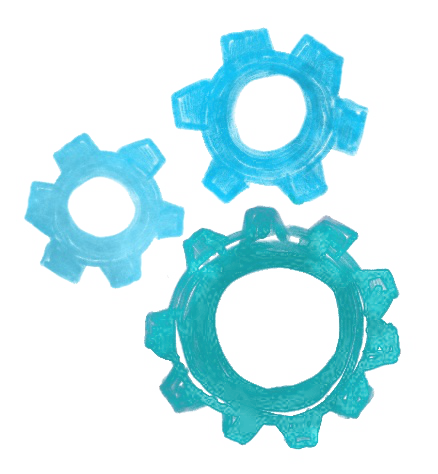
\includegraphics[height=.6cm]{images/gears.png}} \large \textcolor{deffun-text}{Definition-Box: #1}\\
    }
    {
  \end{mybox}
  }

% design
\newenvironment{design}[1][Title]
  {
  \setlength{\fboxsep}{1em}
  \begin{mybox}[design-line]
    \raisebox{-.2\height}{
\includegraphics[height=.6cm]{images/design.png}} \large \textcolor{design-text}{Approfondimento: #1}\\
    }
    {
  \end{mybox}
  }

% trick
\newenvironment{trick}[1][Title]
  {
  \setlength{\fboxsep}{1em}
  \begin{mybox}[trick-line]
    \raisebox{-.2\height}{
\includegraphics[height=.6cm]{images/hat.png}} \large \textcolor{trick-text}{Trick-Box: #1}\\
    }
    {
  \end{mybox}
  }
\usepackage{titlepic}
\titlepic{
\includegraphics[width=\textwidth]{images/logo_psicostat.pdf}}
\usepackage{booktabs}
\usepackage{longtable}
\usepackage{array}
\usepackage{multirow}
\usepackage{wrapfig}
\usepackage{float}
\usepackage{colortbl}
\usepackage{pdflscape}
\usepackage{tabu}
\usepackage{threeparttable}
\usepackage{threeparttablex}
\usepackage[normalem]{ulem}
\usepackage{makecell}
\usepackage{xcolor}
\usepackage[]{natbib}
\bibliographystyle{plainnat}

\title{{Introduzione a R}}
\usepackage{etoolbox}
\makeatletter
\providecommand{\subtitle}[1]{% add subtitle to \maketitle
  \apptocmd{\@title}{\par {\large #1 \par}}{}{}
}
\makeatother
\subtitle{Corso per imparare le basi di \textbf{R}}
\author{\href{https://psicostat.dpss.psy.unipd.it/}{Psicostat}}
\date{19-03-2021}

\begin{document}
\maketitle

{
\setcounter{tocdepth}{1}
\tableofcontents
}
\hypertarget{presentazione}{%
\chapter*{Presentazione}\label{presentazione}}
\addcontentsline{toc}{chapter}{Presentazione}

In questo libro impareremo le basi di \emph{R}, uno dei migliori software per la visualizzazione e l'analisi statistica dei dati. Partiremo da zero intorducendo gli aspetti fondamentili di R e i concetti alla base di ogni linguaggio di programmazione che ti pemetteranno in seguito di approfondire e sviluppare le tue abilità in questo bellissimo mondo.

\hypertarget{perchuxe8-r}{%
\section*{Perchè R}\label{perchuxe8-r}}
\addcontentsline{toc}{section}{Perchè R}

Ci sono molte ragioni per cui scegliere R rispetto ad altri programmi usati per condurre le analisi statistiche. Innanzitutto è un linguaggio di programmazione (come ad esempio Python, Java, C++, o Julia) e non semplicemente un'interfaccia punta e clicca (come ad esempio SPSS o JASP). Questo comporta si maggiori difficoltà iniziali ma ti ricompenserà in futuro poichè avari imparato ad utilizza uno strumennto molto potente.

Inoltre, R è:

\begin{itemize}
\tightlist
\item
  nato per la statistica
\item
  open-source
\item
  ricco di pacchetti
\item
  supportato da una grande community
\item
  gratis
\end{itemize}

\hypertarget{struttura-del-libro}{%
\section*{Struttura del libro}\label{struttura-del-libro}}
\addcontentsline{toc}{section}{Struttura del libro}

Il libro è suddiviso in quattro sezioni principali:

\begin{itemize}
\tightlist
\item
  \textbf{Get started}. Una volta installato R ed RStudio, famiglierizzeremo con l'ambiente di lavoro introducendo alcuni aspetti generali e le funzioni principali. Verranno inoltre descritte alcune buone regole per iniziare una sessione di lavoro in R.
\item
  \textbf{Struttura dei dati}. Impareremo gli oggetti principali che R utilizza al suo interno. Variabili, vettori, matrici, dataframe e liste non avranno più segreti e capiremo come manipolarli e utlizzarli a seconda delle varie necessità.
\item
  \textbf{Algoritmi}. Non farti spaventare da questo nome. Ne avrai spesso sentito parlarne come qualcosa di molto complicato, ma in realtà gli algoritmi sono semplicemente una serie di istruzioni che il computer segue quando deve eseguire un determinato compito. In questa sezione vedremo i principali comandi di R usati per definire degli algoritmi. Questo è il vantaggio di conoscere un linguaggio di programmazione, ci permette di creare nuovi programmi che il computer eseguirà per noi.
\item
  \textbf{Case study}. Eseguiremo passo per passo un analisi che ci permetterà di imparare come importare i dati, codificare le variabili, manipolare e preprare i dati perle analisi, condurre delle analisi descrittive e creare dei grafici.
\end{itemize}

Alla fine di questo libro probabilmente non sarete assunti da Google, ma speriamo almeno che R non vi faccia più così paura e che magari a qualcuno sia nato l'interesse di approfondire questo fantastico mondo fatto di linee di codice.

\hypertarget{risorse-utili}{%
\section*{Risorse Utili}\label{risorse-utili}}
\addcontentsline{toc}{section}{Risorse Utili}

Segnaliamo qui per il lettore interessato del materiale online (in inglese) per approfondire le conoscenze sull'uso di R.

Materiale introduttivo:

\begin{itemize}
\tightlist
\item
  \emph{R for Psychological Science} di Danielle Navarro \url{https://psyr.djnavarro.net/index.html}
\item
  \emph{Hands-On Programming with R} di Garrett Grolemund \url{https://rstudio-education.github.io/hopr/}
\end{itemize}

Materiale intermedio:

\begin{itemize}
\tightlist
\item
  \emph{R for Data Science} di Hadley Wickham e Garrett Grolemund \url{https://r4ds.had.co.nz/}
\end{itemize}

Materiale avanzato:

\begin{itemize}
\tightlist
\item
  \emph{R Packages} di Hadley Wickham e Jennifer Bryan \url{https://r-pkgs.org/}
\item
  \emph{Advanced R} di Hadley Wickham \url{https://adv-r.hadley.nz/}
\end{itemize}

\hypertarget{psicostat}{%
\section*{Psicostat}\label{psicostat}}
\addcontentsline{toc}{section}{Psicostat}

Questo libro è stato prodotto da \textbf{Psicostat}, un gruppo di ricerca interdisciplinare dell'universita di Padova che unisce la passione per la statistica e la psicologia. Se vuoi conoscere di più riguardo le nostre attività visita il nosto sito \url{https://psicostat.dpss.psy.unipd.it/} o aggiungiti alla nostra mailing list \url{https://lists.dpss.psy.unipd.it/postorius/lists/psicostat.lists.dpss.psy.unipd.it/}.

\hypertarget{collaborazione}{%
\section*{Collaborazione}\label{collaborazione}}
\addcontentsline{toc}{section}{Collaborazione}

Se vuoi collaborare alla revione e scrittura di questo libro (ovviamente è tutto in R) visita la nostra repository di Github \url{https://github.com/psicostat/Introduction2R}.

\hypertarget{riconoscimenti}{%
\section*{Riconoscimenti}\label{riconoscimenti}}
\addcontentsline{toc}{section}{Riconoscimenti}

Il template di questo libro è basato su \href{https://github.com/rstudio/bookdown-demo}{Rstudio Bookdown-demo} rilasciato con licenza \href{https://creativecommons.org/publicdomain/zero/1.0/}{CC0-1.0} e \href{https://rstudio4edu.github.io/rstudio4edu-book/}{rstudio4edu-book} rilasciato con licenza \href{https://creativecommons.org/licenses/by/2.0/}{CC BY}. Nota che le illustrazioni utilizzate nelle vignette appartengono sempre a \href{https://rstudio4edu.github.io/rstudio4edu-book/}{rstudio4edu-book} e sono rilasciate con licenza \href{https://creativecommons.org/licenses/by-nc/2.0/}{CC BY-NC}.

\hypertarget{licenza}{%
\section*{Licenza}\label{licenza}}
\addcontentsline{toc}{section}{Licenza}

Questo libro è rilasciato sotto la Creative Commons Attribution-ShareAlike 4.0 International Public License (\href{https://creativecommons.org/licenses/by-sa/4.0/legalcode}{CC BY-SA}).
Le illustrazioni utilizzate nelle vignette appartengono a \href{https://rstudio4edu.github.io/rstudio4edu-book/}{rstudio4edu-book} e sono rilasciate con licenza \href{https://creativecommons.org/licenses/by-nc/2.0/}{CC BY-NC}.

\hypertarget{part-get-started}{%
\part*{Get Started}\label{part-get-started}}
\addcontentsline{toc}{part}{Get Started}

\hypertarget{intorduzione}{%
\chapter*{Intorduzione}\label{intorduzione}}
\addcontentsline{toc}{chapter}{Intorduzione}

In questa sezione verranno presentate le istruzioni per installare R ed RStudio. In seguito, famiglierizzeremo con l'ambiente di lavoro introducendo alcuni aspetti generali e le funzioni principali. Verranno inoltre descritte alcune buone regole per iniziare una sessione di lavoro in R.

I capitoli sono così organizzati:

\begin{itemize}
\tightlist
\item
  \textbf{Capitolo \ref{install} - Installare R e RStudio}. Instruzioni passo a passo per installare R e RStudio
\item
  \textbf{Capitolo \ref{rstudio-gui} - Interfaccia RStudio}. Introduzione all'interfaccia utente di RStudio.
\item
  \textbf{Capitolo \ref{first-comands} - Primi Passi in R}. Operatori matematici, operatori relazionali, operatori logici.
\item
  \textbf{Capitolo \ref{objects-functions} - Due Compagni Inseparabili}. Introduzione dei concetti di oggetti e funzioni in R.
\item
  \textbf{Capitolo \ref{working-session} - Sessione di Lavoro}. Utilizzo degli script e introduzione dei concetti di working directory e pacchetti di R.
\end{itemize}

\hypertarget{install}{%
\chapter{Installare R e RStudio}\label{install}}

R ed R-studio sono due software distinti. R è un linguaggio di programmazione usato in particolare in ambiti quali la statistica. R-studio invece è un'interfaccia \emph{user-friendly} che permette di utilizzare R.
R può essere utilizzato autonomamente tuttavia è consigliato l'utilizzo attraverso R-studio. Entrambi vanno installati separatamente e la procedura varia a seconda del proprio sistema operativo (Windows, MacOS o Linux). Riportiamo le istruzioni solo per Windows e MacOS Linux (Ubuntu). Ovviamente R è disponibile per tutte le principali distribuzioni di Linux. Le istruzioni riportate per Ubuntu (la distribuzione più diffusa) sono valide anche per le distribuzioni derivate.

\hypertarget{installare-r}{%
\section{Installare R}\label{installare-r}}

\begin{enumerate}
\def\labelenumi{\arabic{enumi}.}
\tightlist
\item
  Accedere al sito \url{https://www.r-project.org}
\item
  Selezionare la voce \textbf{CRAN} (Comprehensive R Archive Network) dal menù di sinistra sotto \textbf{Download}
\end{enumerate}

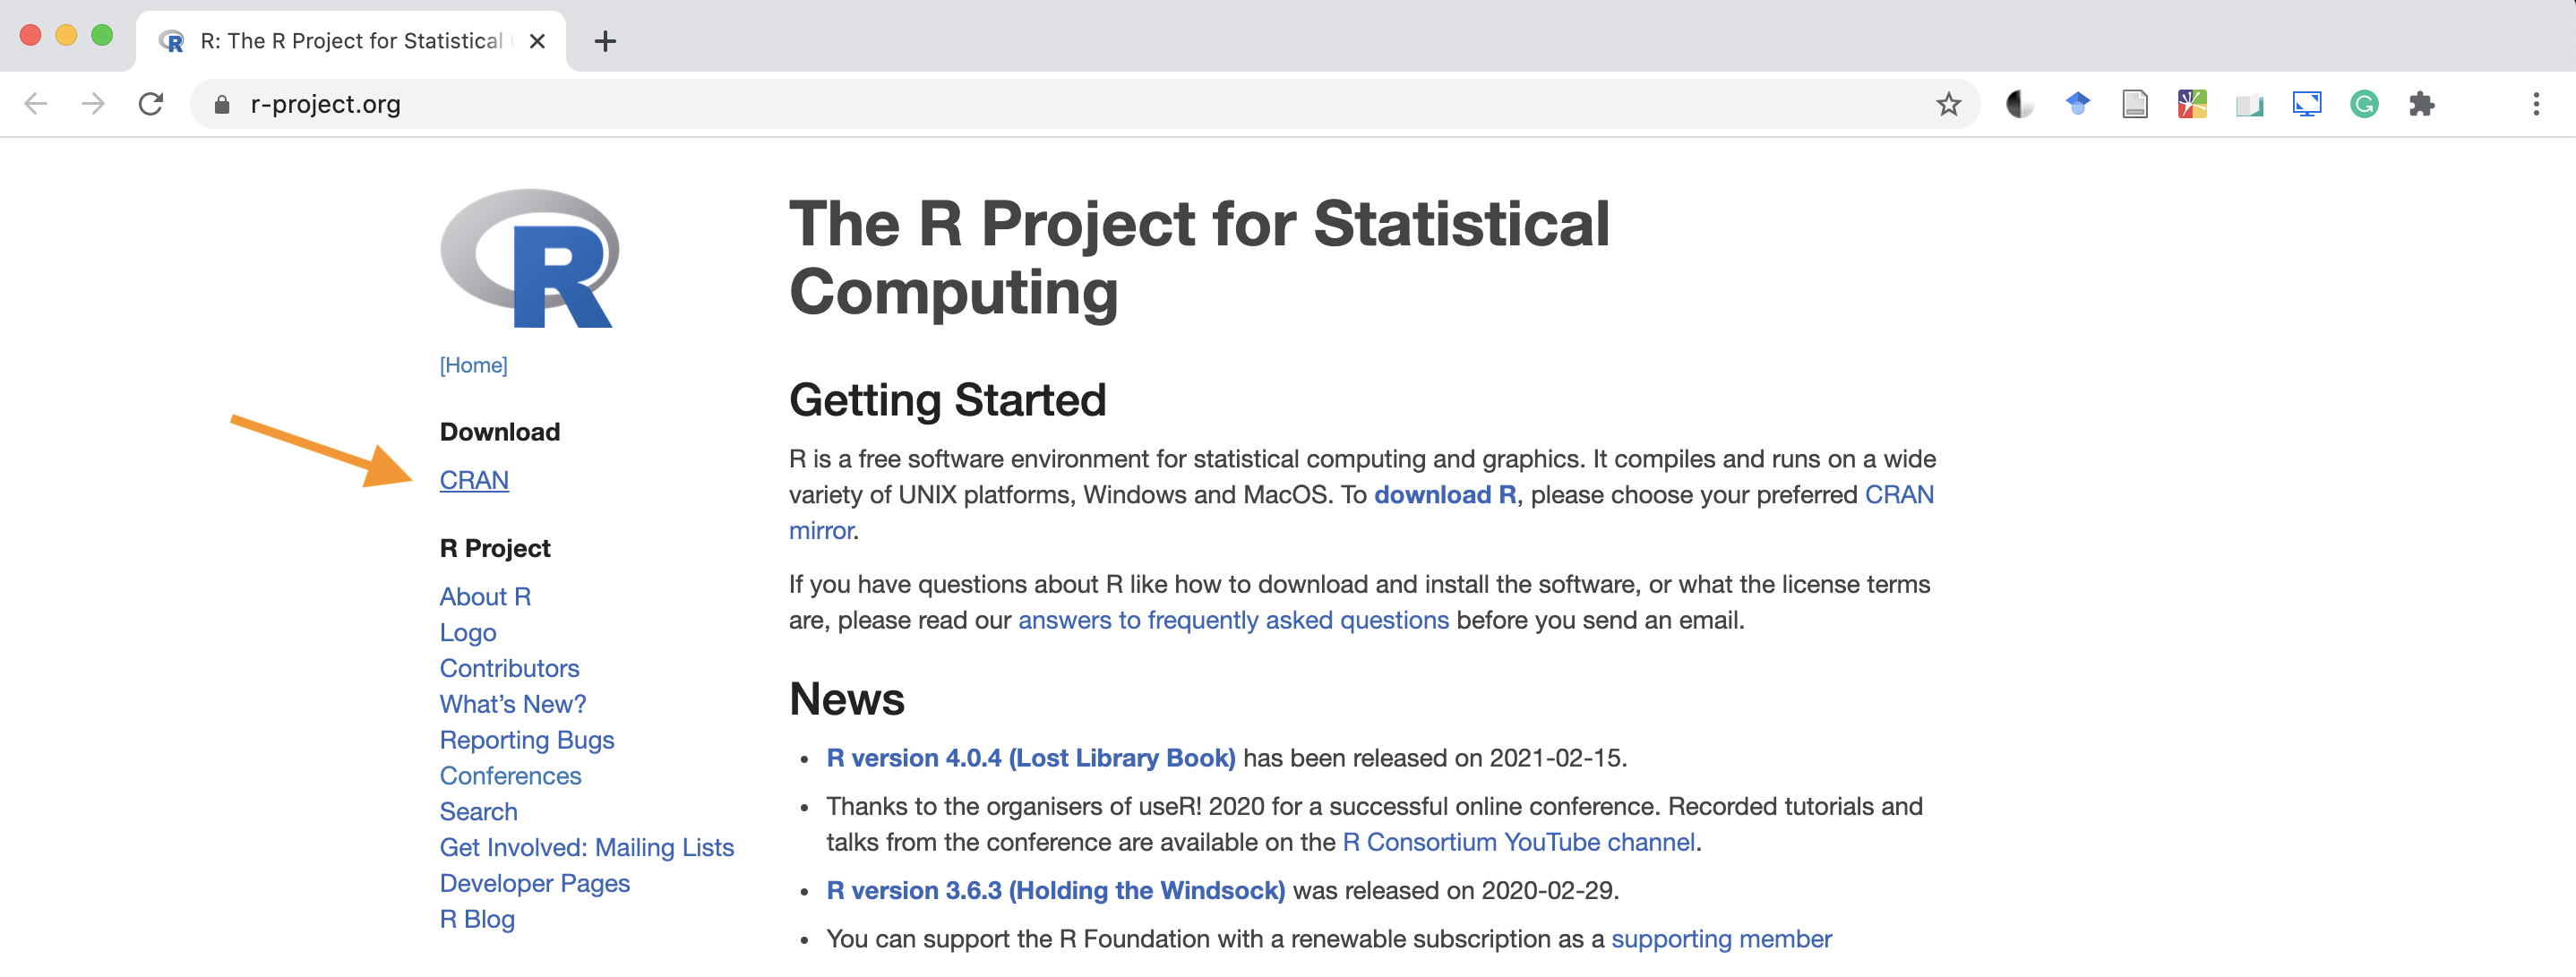
\includegraphics[width=0.95\textwidth,height=\textheight]{images/install_CRAN.png}

\begin{enumerate}
\def\labelenumi{\arabic{enumi}.}
\setcounter{enumi}{2}
\tightlist
\item
  Selezionare il primo link \url{https://cloud.r-project.org/}
\end{enumerate}

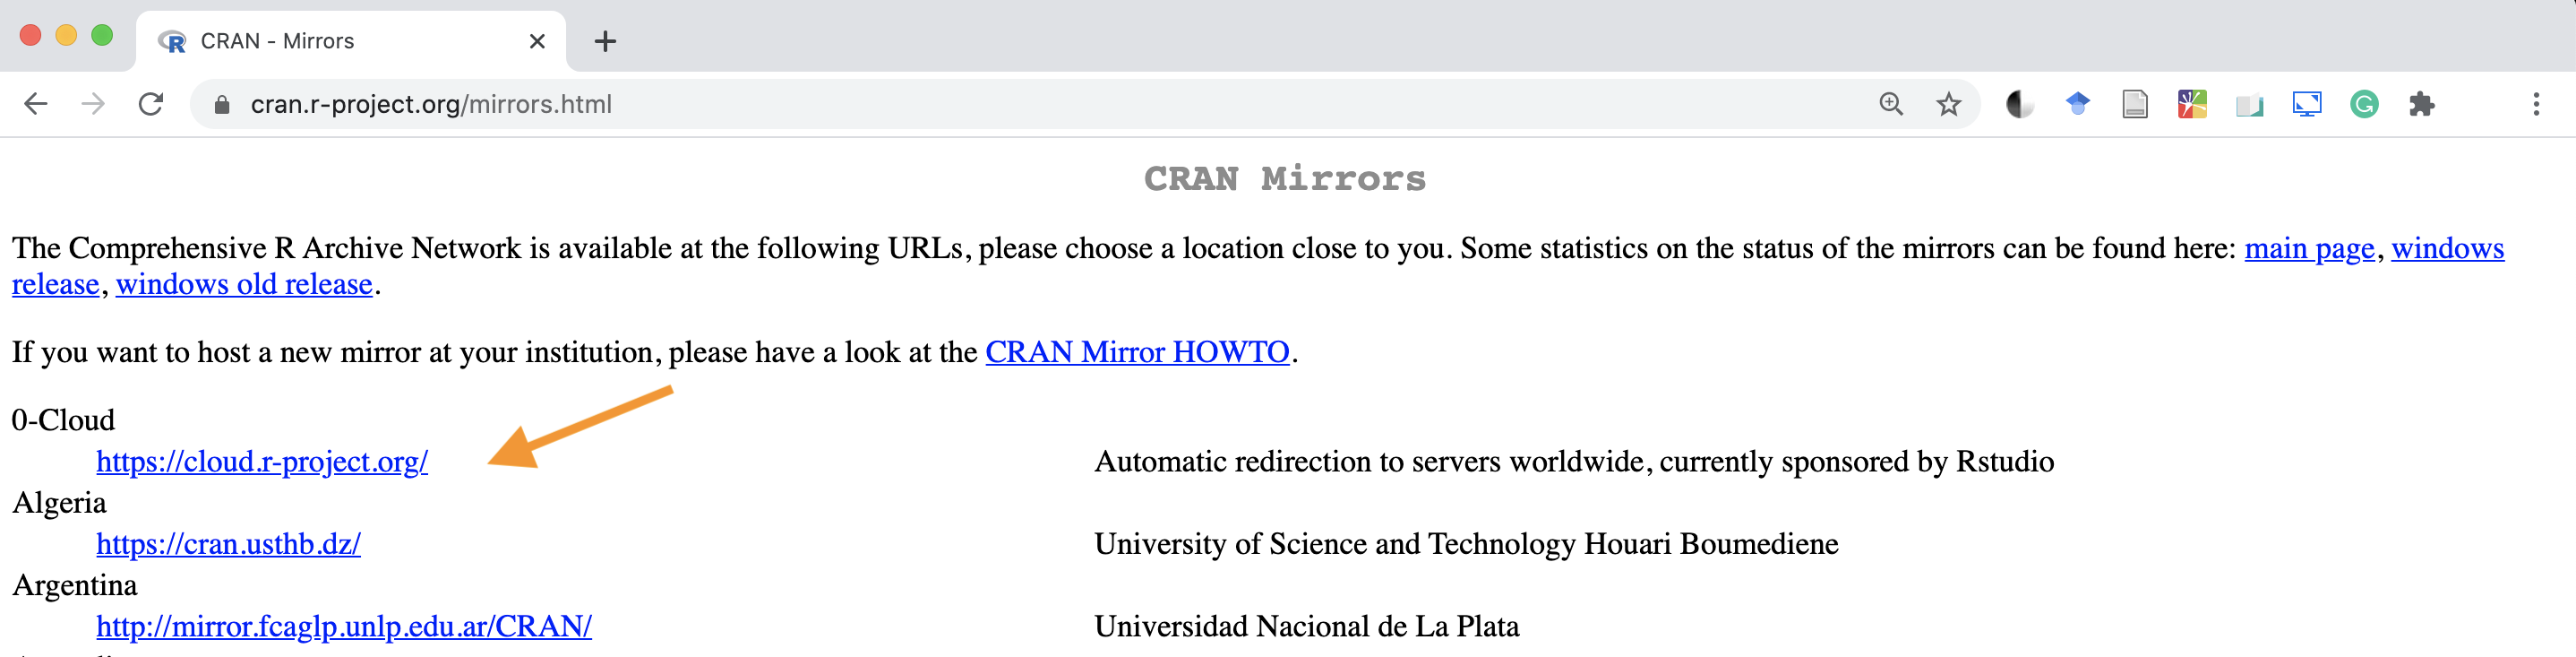
\includegraphics[width=0.95\textwidth,height=\textheight]{images/install_mirror.png}

\begin{enumerate}
\def\labelenumi{\arabic{enumi}.}
\setcounter{enumi}{3}
\tightlist
\item
  Selezionare il proprio sistema operativo
\end{enumerate}

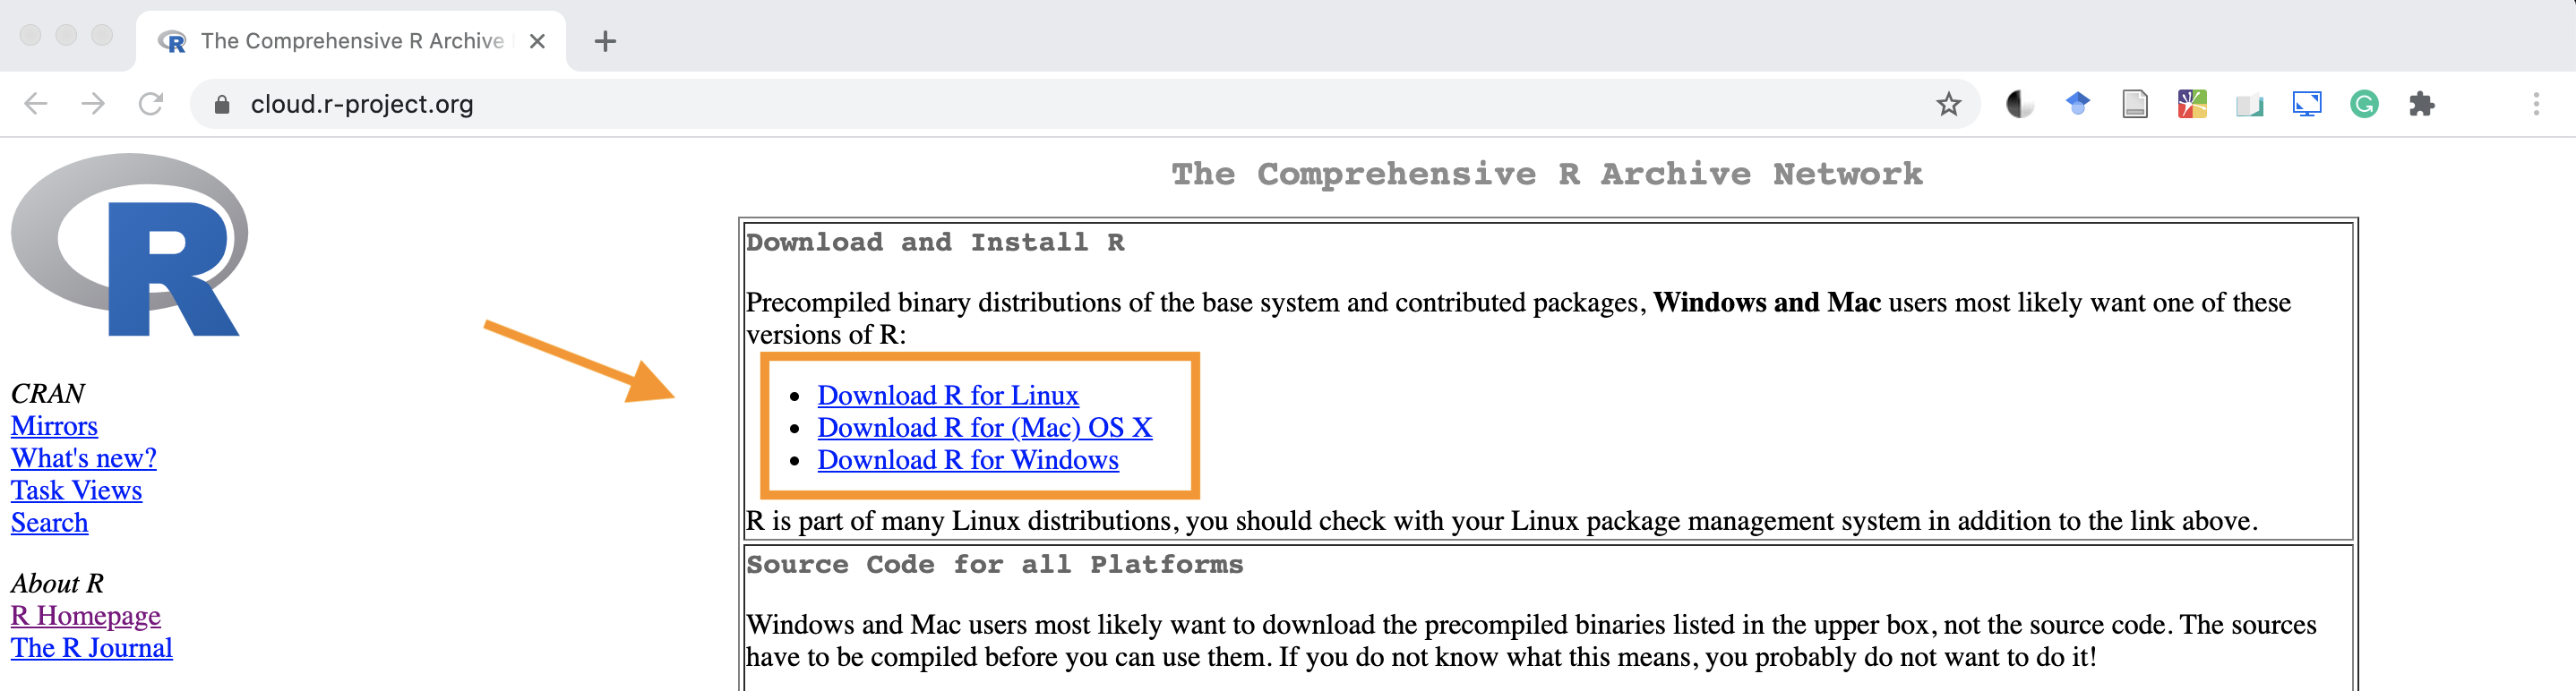
\includegraphics[width=0.95\textwidth,height=\textheight]{images/install_OS.png}

\hypertarget{r-windows}{%
\subsection{R Windows}\label{r-windows}}

\begin{enumerate}
\def\labelenumi{\arabic{enumi}.}
\tightlist
\item
  Selezionare la voce \textbf{base}
\end{enumerate}

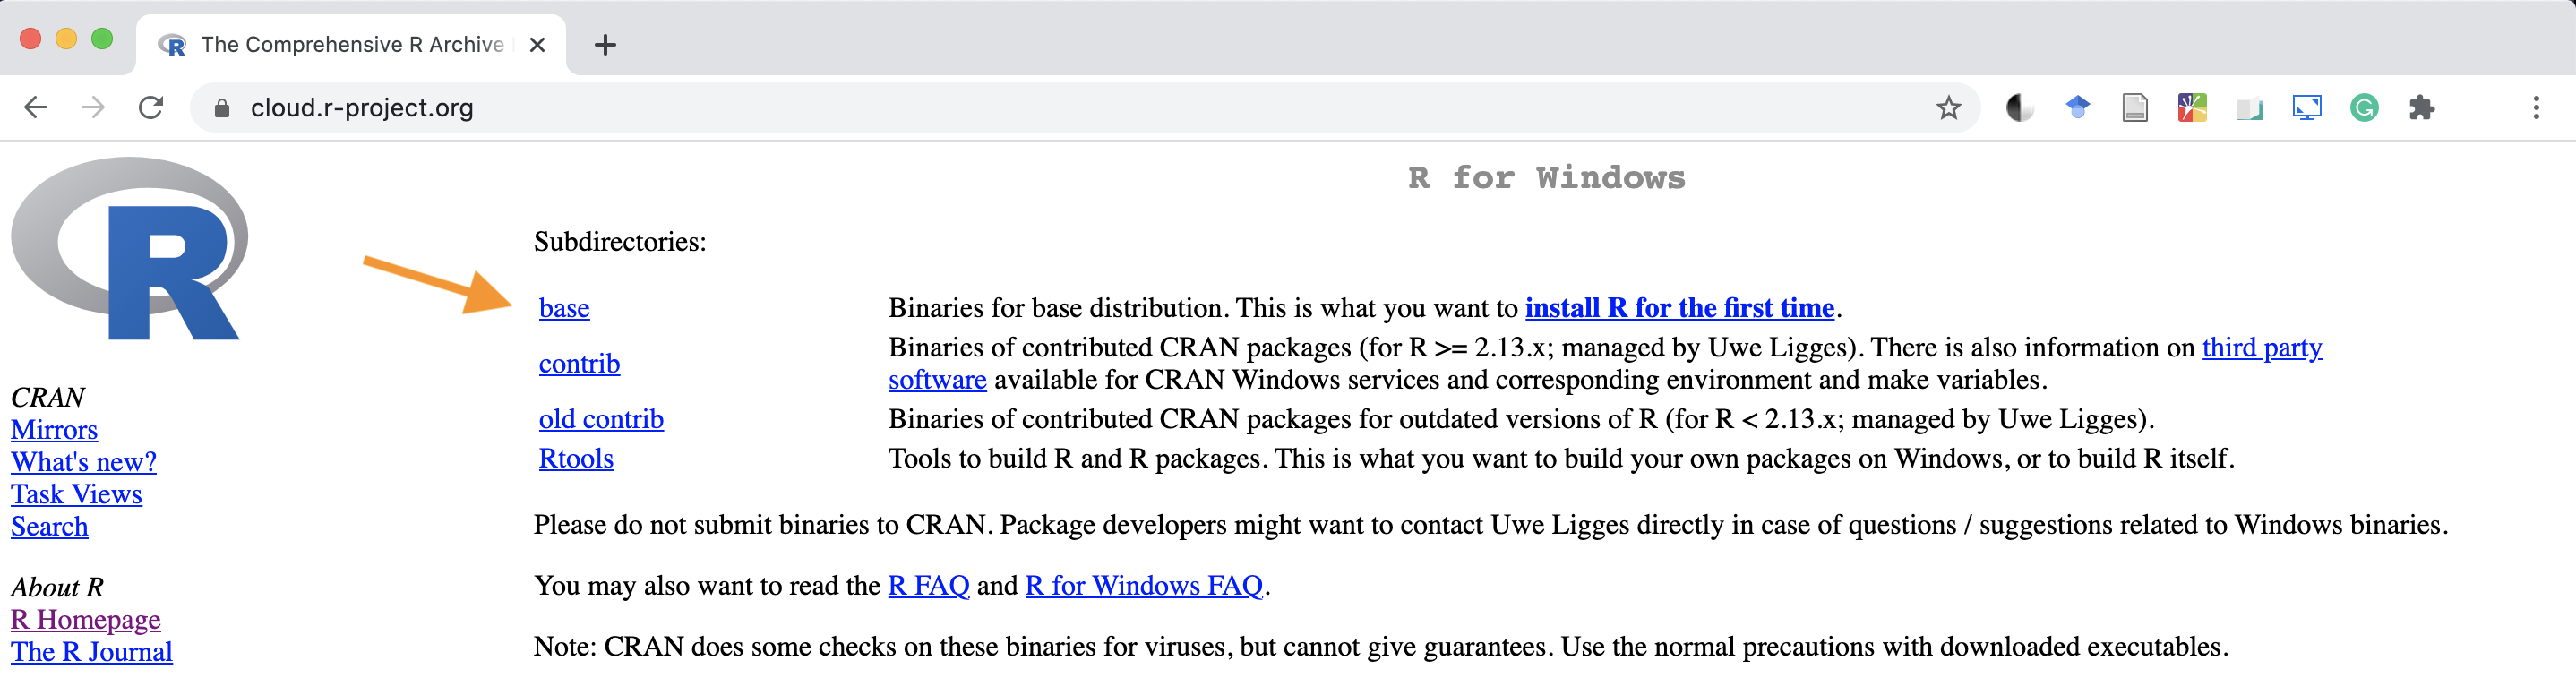
\includegraphics[width=0.95\textwidth,height=\textheight]{images/install-Windows-base.png}

\begin{enumerate}
\def\labelenumi{\arabic{enumi}.}
\setcounter{enumi}{1}
\tightlist
\item
  Selezionare la voce \textbf{Download} della versione più recente di R disponibile
\end{enumerate}

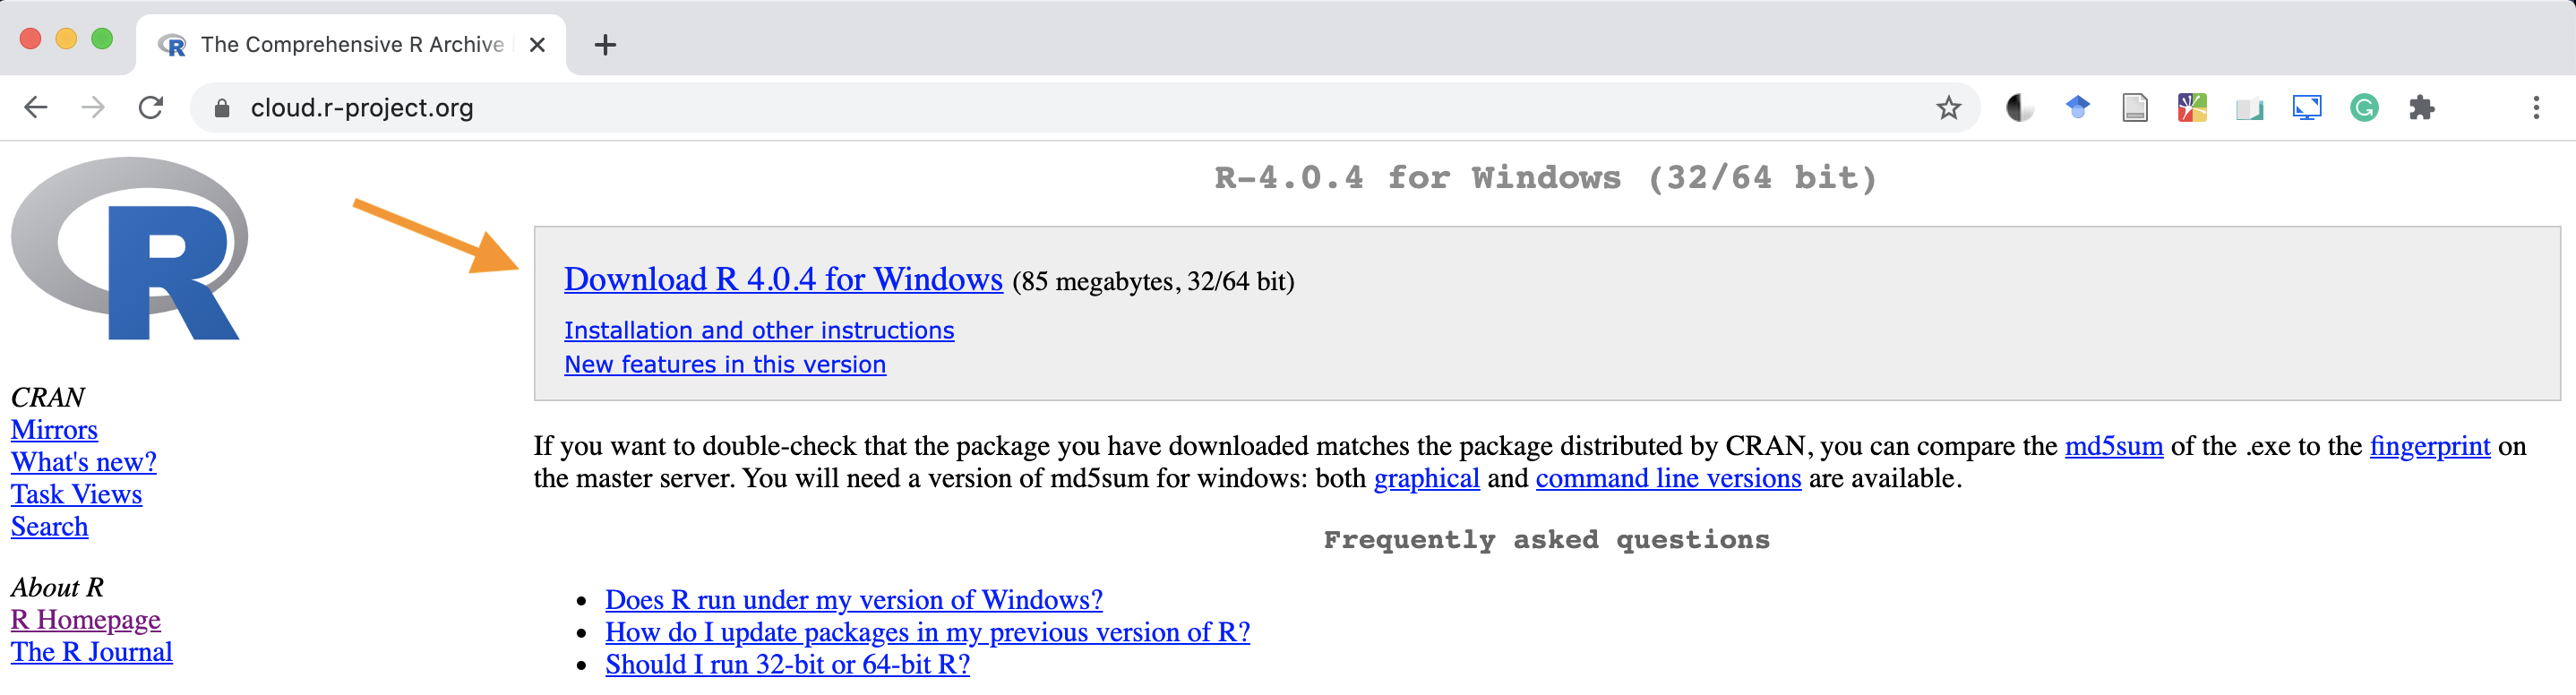
\includegraphics[width=0.95\textwidth,height=\textheight]{images/install-Windows-version.png}

\begin{enumerate}
\def\labelenumi{\arabic{enumi}.}
\setcounter{enumi}{2}
\tightlist
\item
  Al termine del download, eseguire il file e seguire le istruzioni fino al termine dell'installazione
\end{enumerate}

\hypertarget{r-macos}{%
\subsection{R MacOS}\label{r-macos}}

\begin{enumerate}
\def\labelenumi{\arabic{enumi}.}
\tightlist
\item
  Selezionare della versione più recente di R disponibile
\end{enumerate}

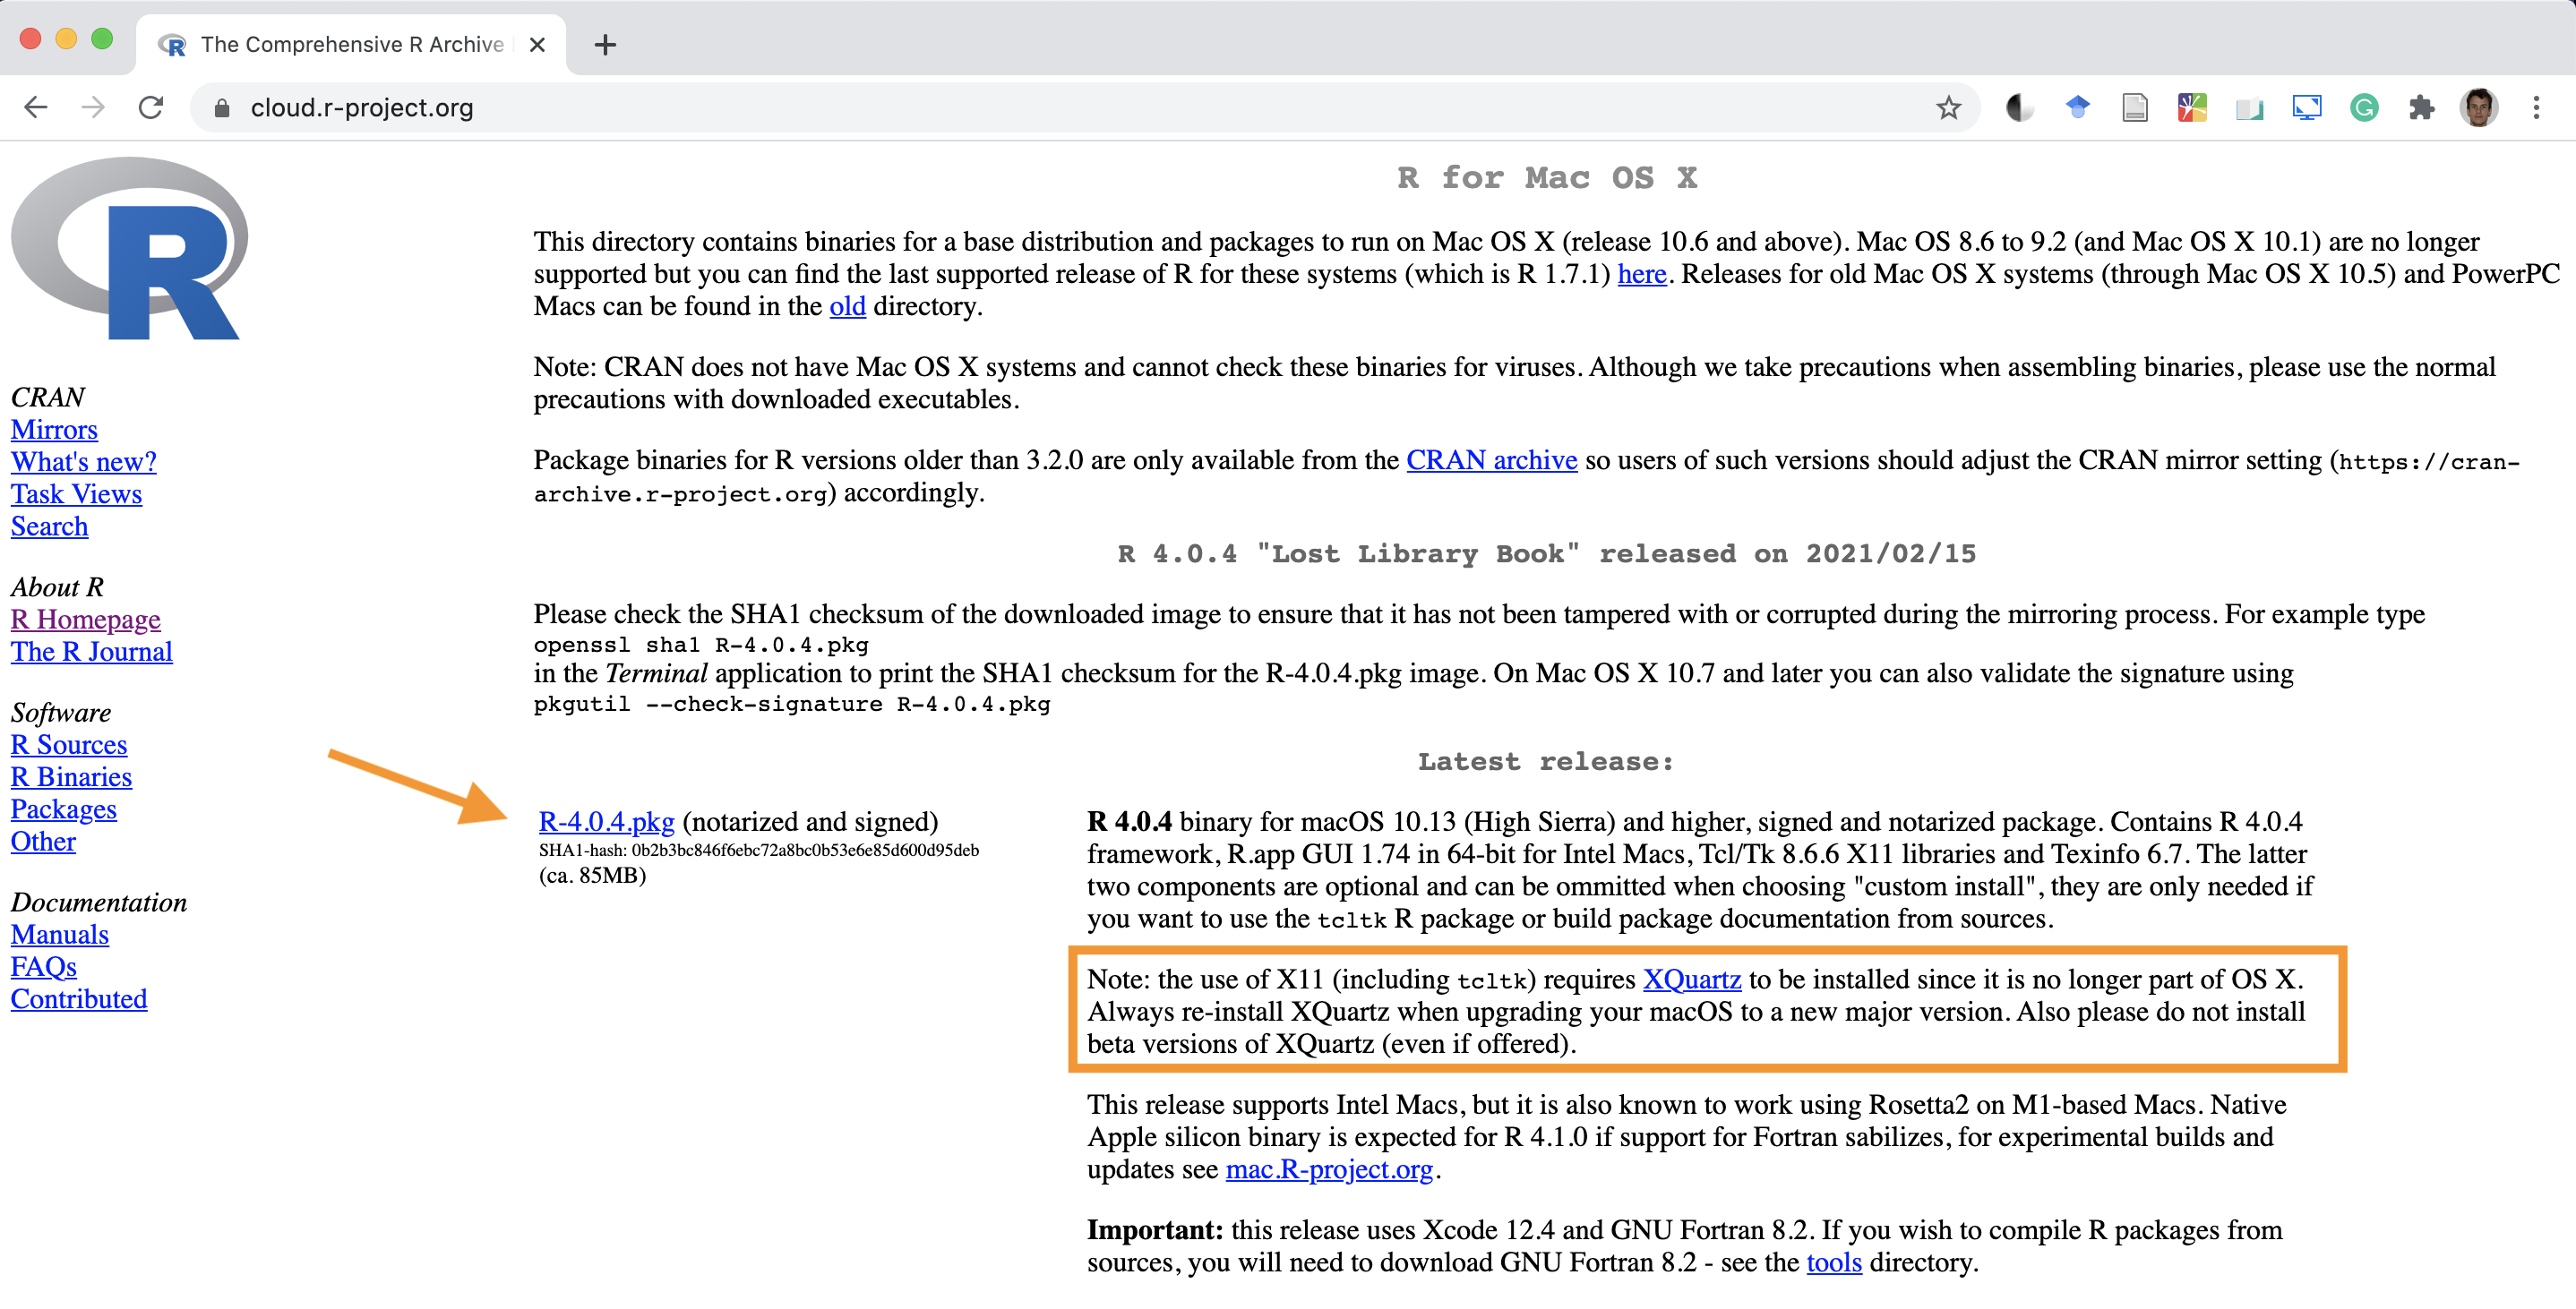
\includegraphics[width=0.95\textwidth,height=\textheight]{images/install_Mac_version.png}

\begin{enumerate}
\def\labelenumi{\arabic{enumi}.}
\setcounter{enumi}{1}
\tightlist
\item
  Al termine del download, eseguire il file e seguire le istruzioni fino al termine dell'installazione di R
\item
  Successivamente è necessario installare anche una componente aggiuntiva \textbf{XQuartz} premendo il link all'interno del riquadro arancione riportato nella figura precedente
\item
  Selezionare la voce Download
\end{enumerate}

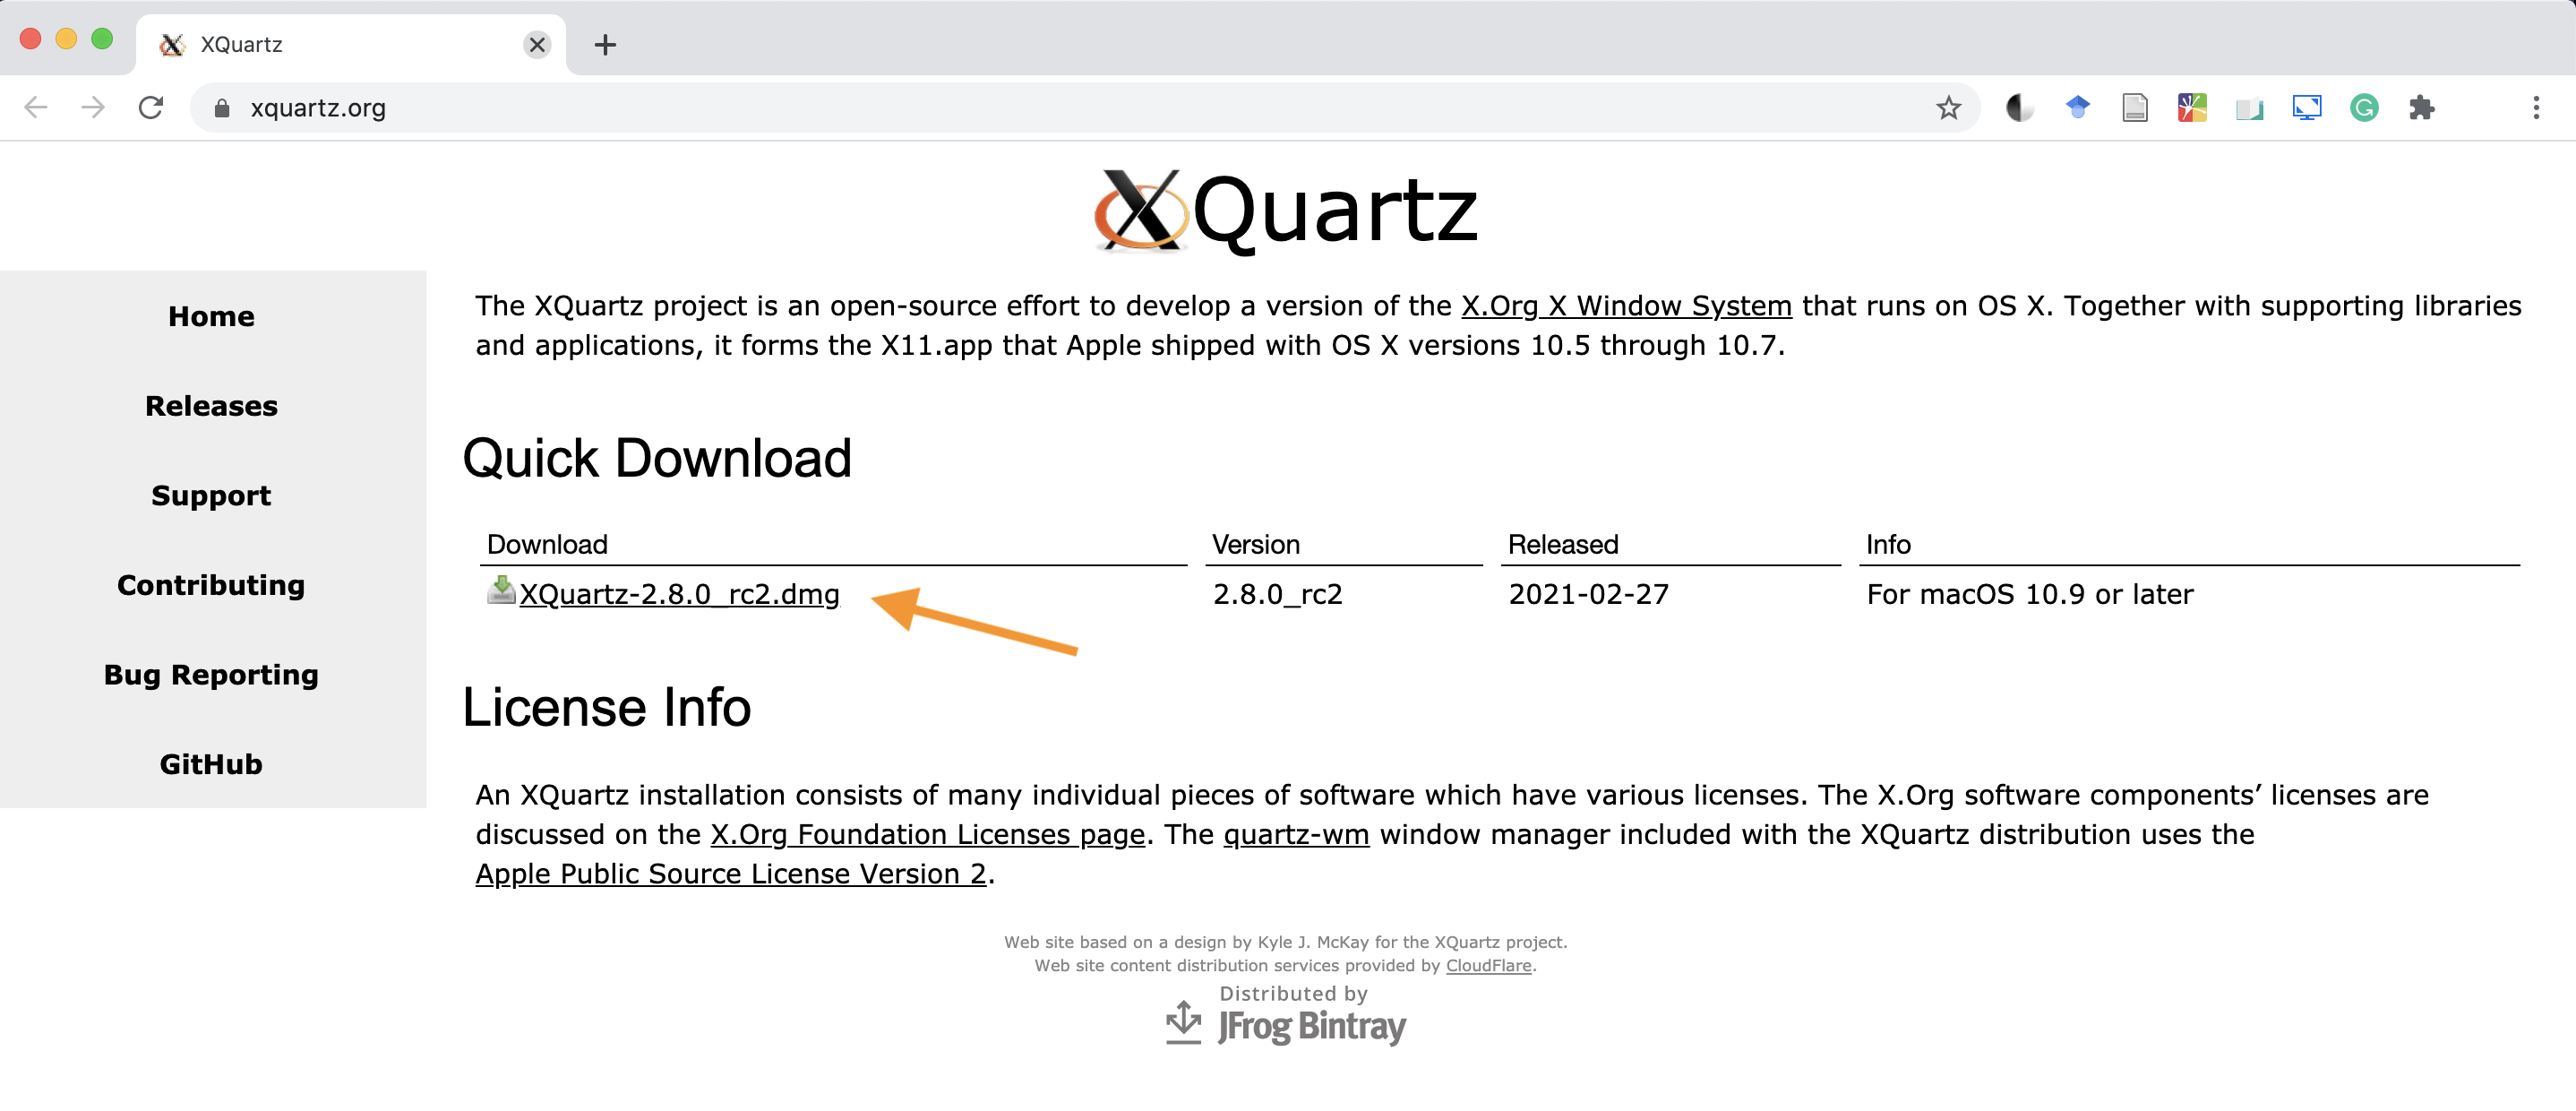
\includegraphics[width=0.95\textwidth,height=\textheight]{images/install_Mac_XQuartz.png}

\begin{enumerate}
\def\labelenumi{\arabic{enumi}.}
\setcounter{enumi}{4}
\tightlist
\item
  Al termine del download, eseguire il file e seguire le istruzioni fino al termine dell'installazione
\end{enumerate}

\hypertarget{r-linux}{%
\subsection{R Linux}\label{r-linux}}

Nonostante la semplicità di installazione di pacchetti su Linux, R a volte potrebbe essere più complicato da installare per via delle diverse distribuzioni, repository e chiavi per riconoscere la repository come sicura.

Sul \textbf{CRAN} vi è la guida ufficiale con tutti i comandi \texttt{apt} da eseguire da terminale. Seguendo questi passaggi non dovrebbero esserci problemi.

\begin{enumerate}
\def\labelenumi{\arabic{enumi}.}
\tightlist
\item
  Andate sul \href{https://cran.r-project.org/}{CRAN}
\item
  Cliccate \texttt{Download\ R\ for\ Linux}
\item
  Selezionate la vostra distribuzione (Ubuntu in questo caso)
\item
  Seguite le istruzioni, principalmente eseguendo i comandi da terminale suggeriti
\end{enumerate}

Per qualsiasi difficoltà o errore, sopratutto con il mondo Linux, una ricerca su online risolve sempre il problema.

\begin{design}[R Tools]

Utilizzi avanzati di R richiedono l'insallazione di una serie ulteriore software definiti \textbf{R tools}.

\hypertarget{windows}{%
\subsubsection*{Windows}\label{windows}}
\addcontentsline{toc}{subsubsection}{Windows}

Seleziona la voce \textbf{Rtools} e segui le istruzioni per completare l'installazione.

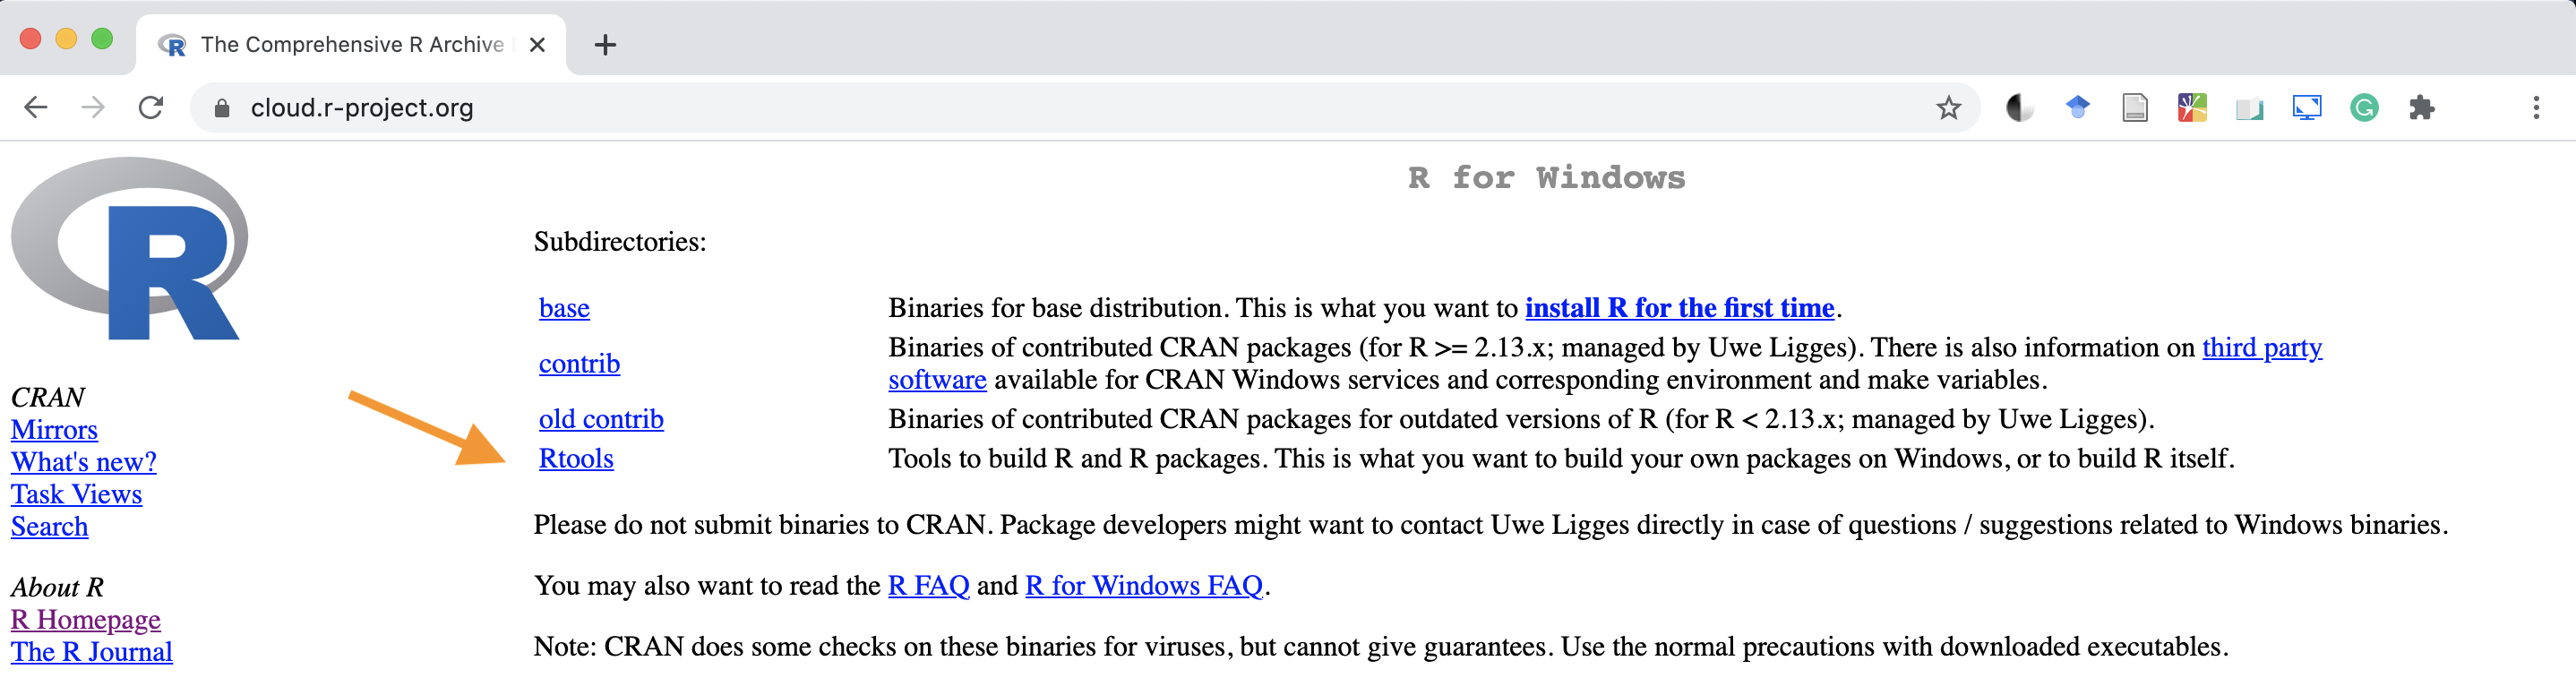
\includegraphics[width=0.95\textwidth,height=\textheight]{images/install-Windows-tools.png}

Nota che sono richieste anche delle operazioni di configurazione affinchè tutto funzioni correttamente.

\hypertarget{macos}{%
\subsubsection*{MacOS}\label{macos}}
\addcontentsline{toc}{subsubsection}{MacOS}

Seleziona la voce \textbf{tools} e segui le istruzioni riportate.

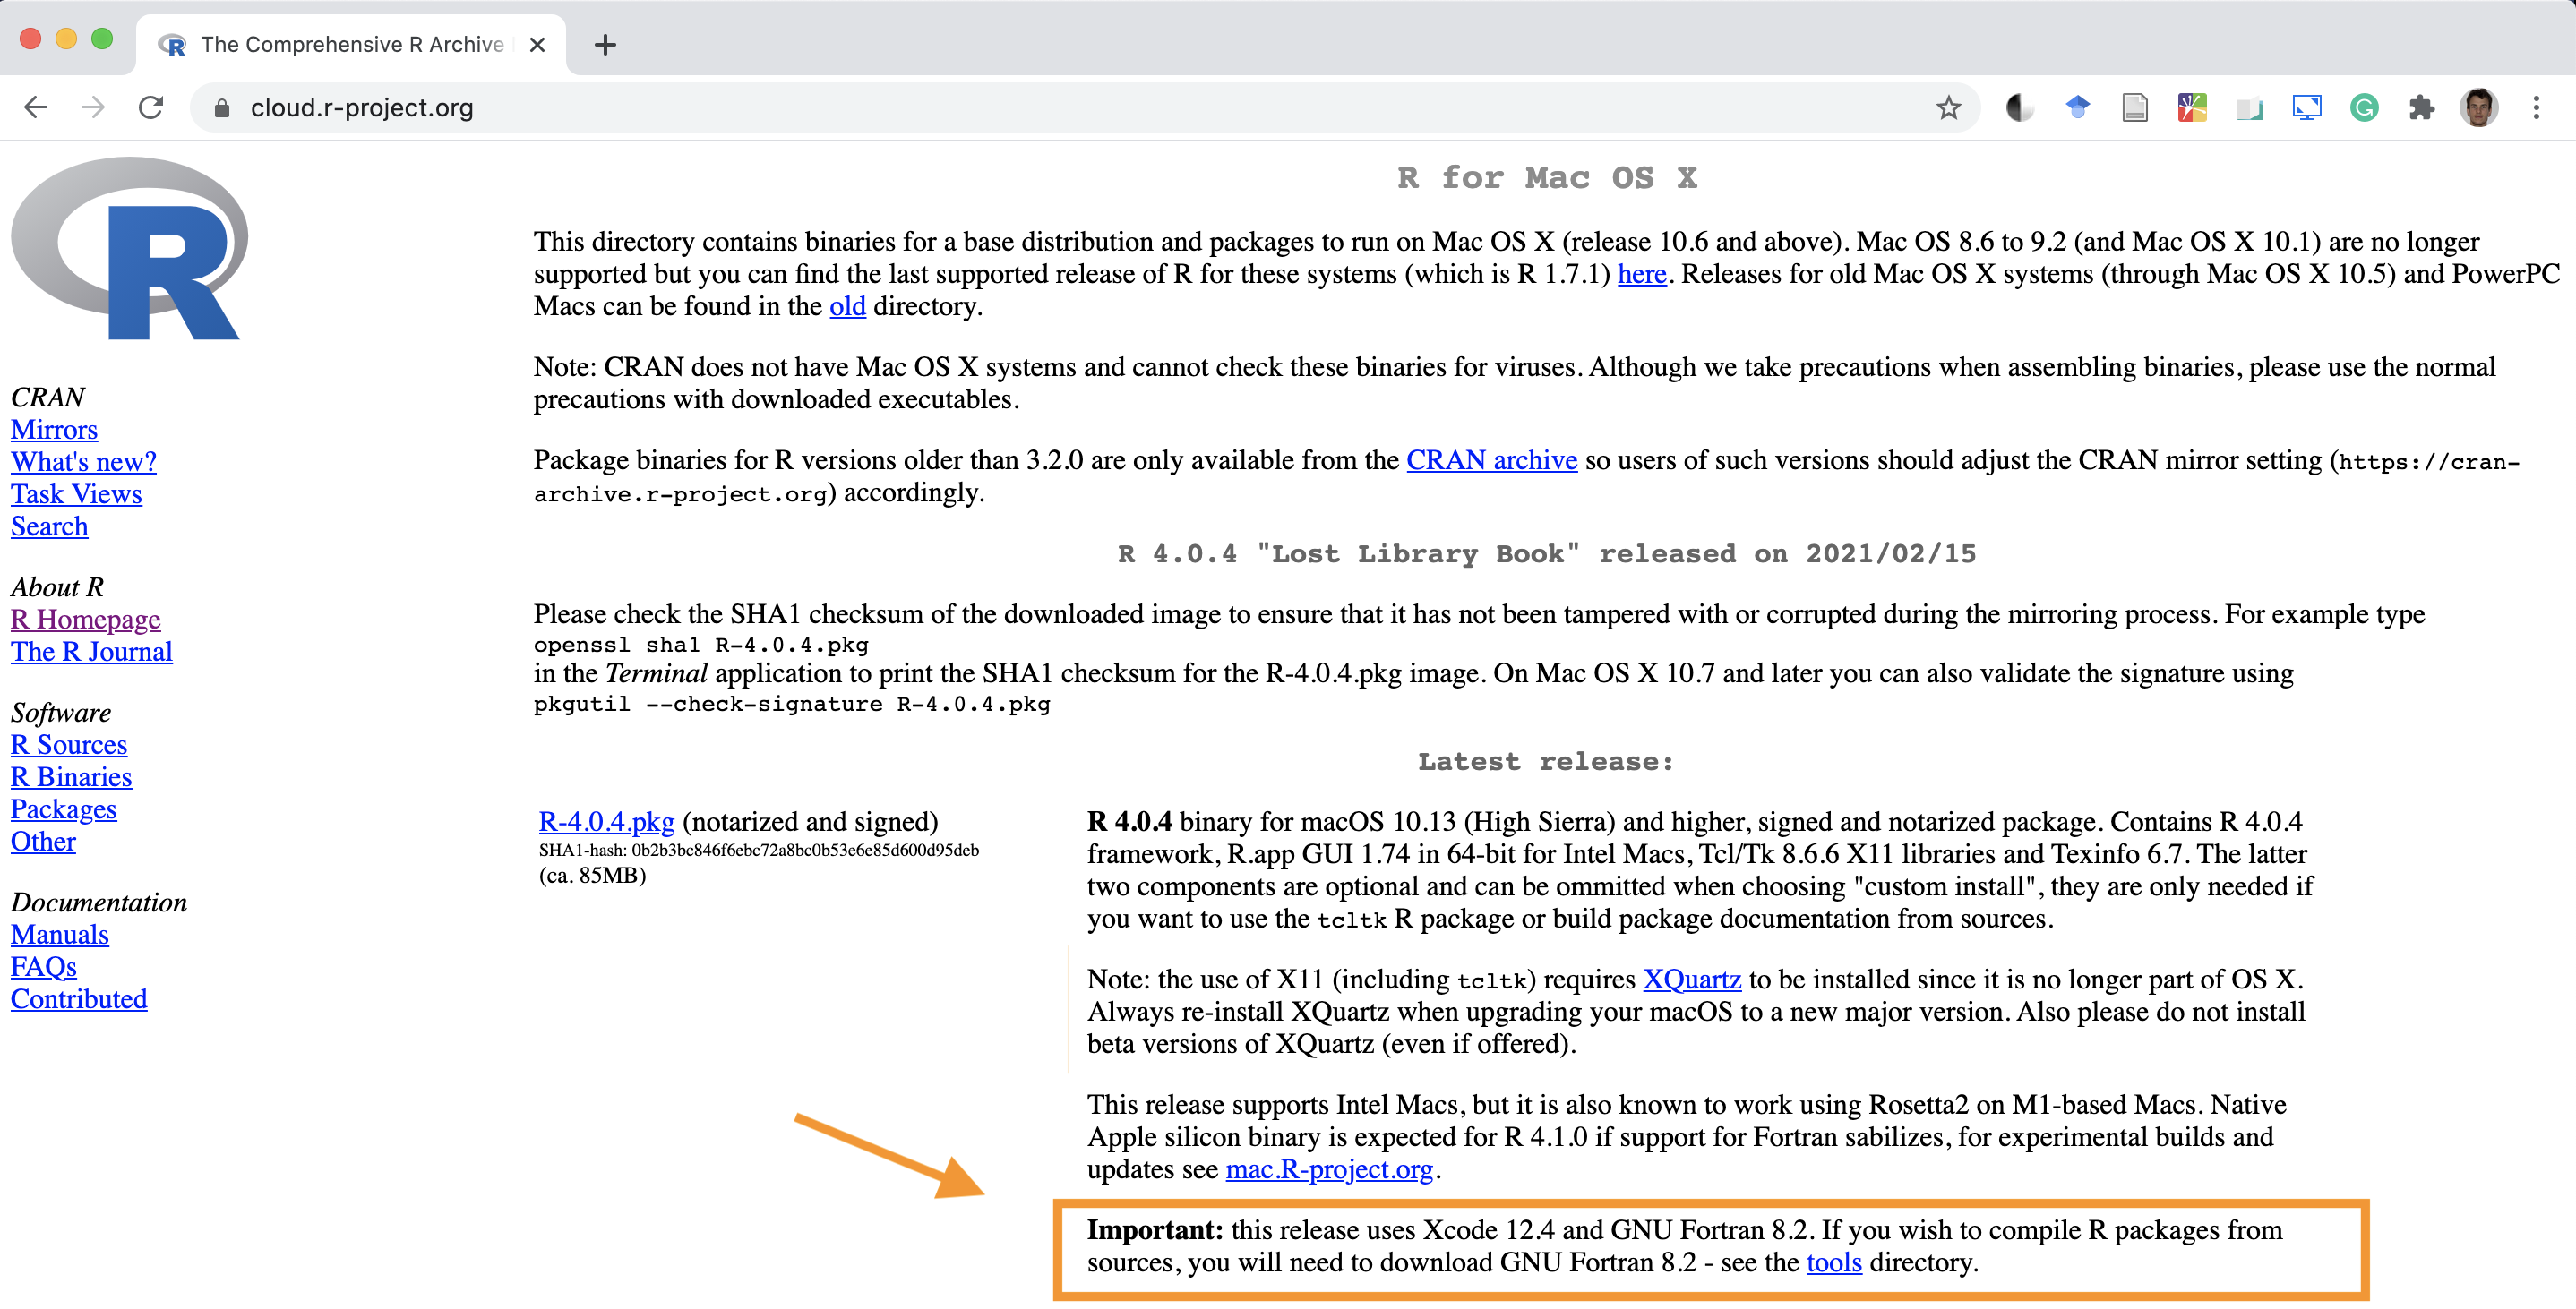
\includegraphics[width=0.95\textwidth,height=\textheight]{images/install_Mac_tools.png}

Nota in particolare che con R 4.0 le seguenti indicazioni sono riportate.


\includegraphics[width=0.95\textwidth,height=\textheight]{images/install_Mac_tools2.png}

\end{design}

\hypertarget{installare-r-studio}{%
\section{Installare R Studio}\label{installare-r-studio}}

\begin{enumerate}
\def\labelenumi{\arabic{enumi}.}
\tightlist
\item
  Accedere al sito \url{https://rstudio.com}
\item
  Selezionare la voce \textbf{DOWNLOAD IT NOW}
\end{enumerate}

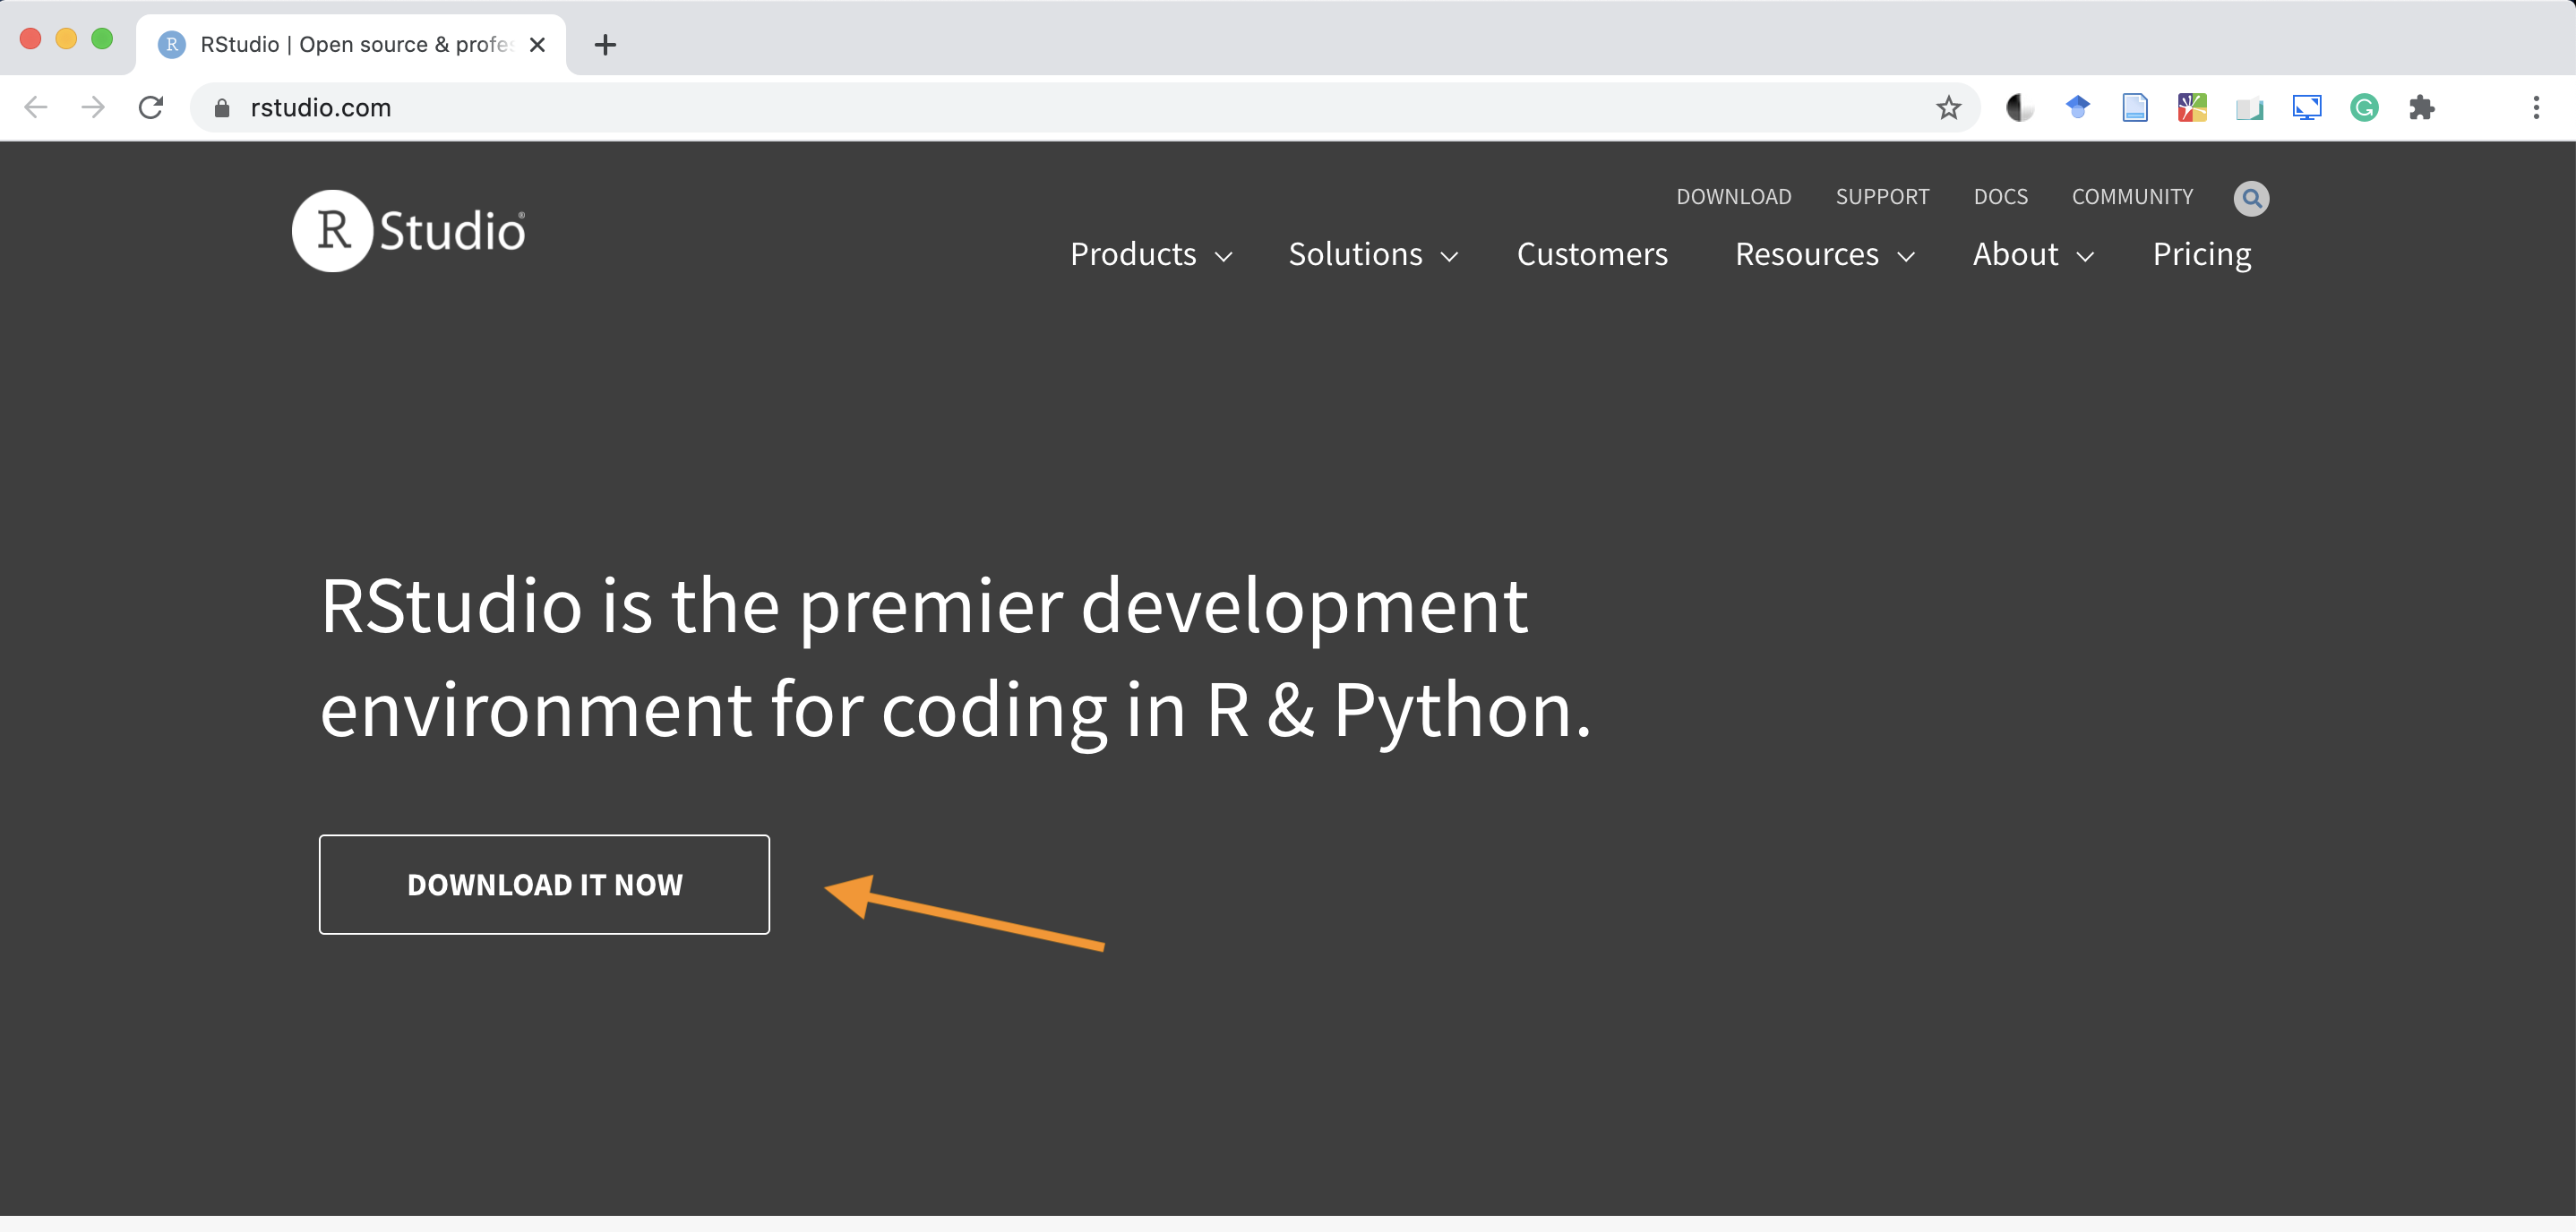
\includegraphics[width=0.95\textwidth,height=\textheight]{images/install_rstudio1.png}

\begin{enumerate}
\def\labelenumi{\arabic{enumi}.}
\setcounter{enumi}{2}
\tightlist
\item
  Selezionare la versione gratuita di RStudio Desktop
\end{enumerate}

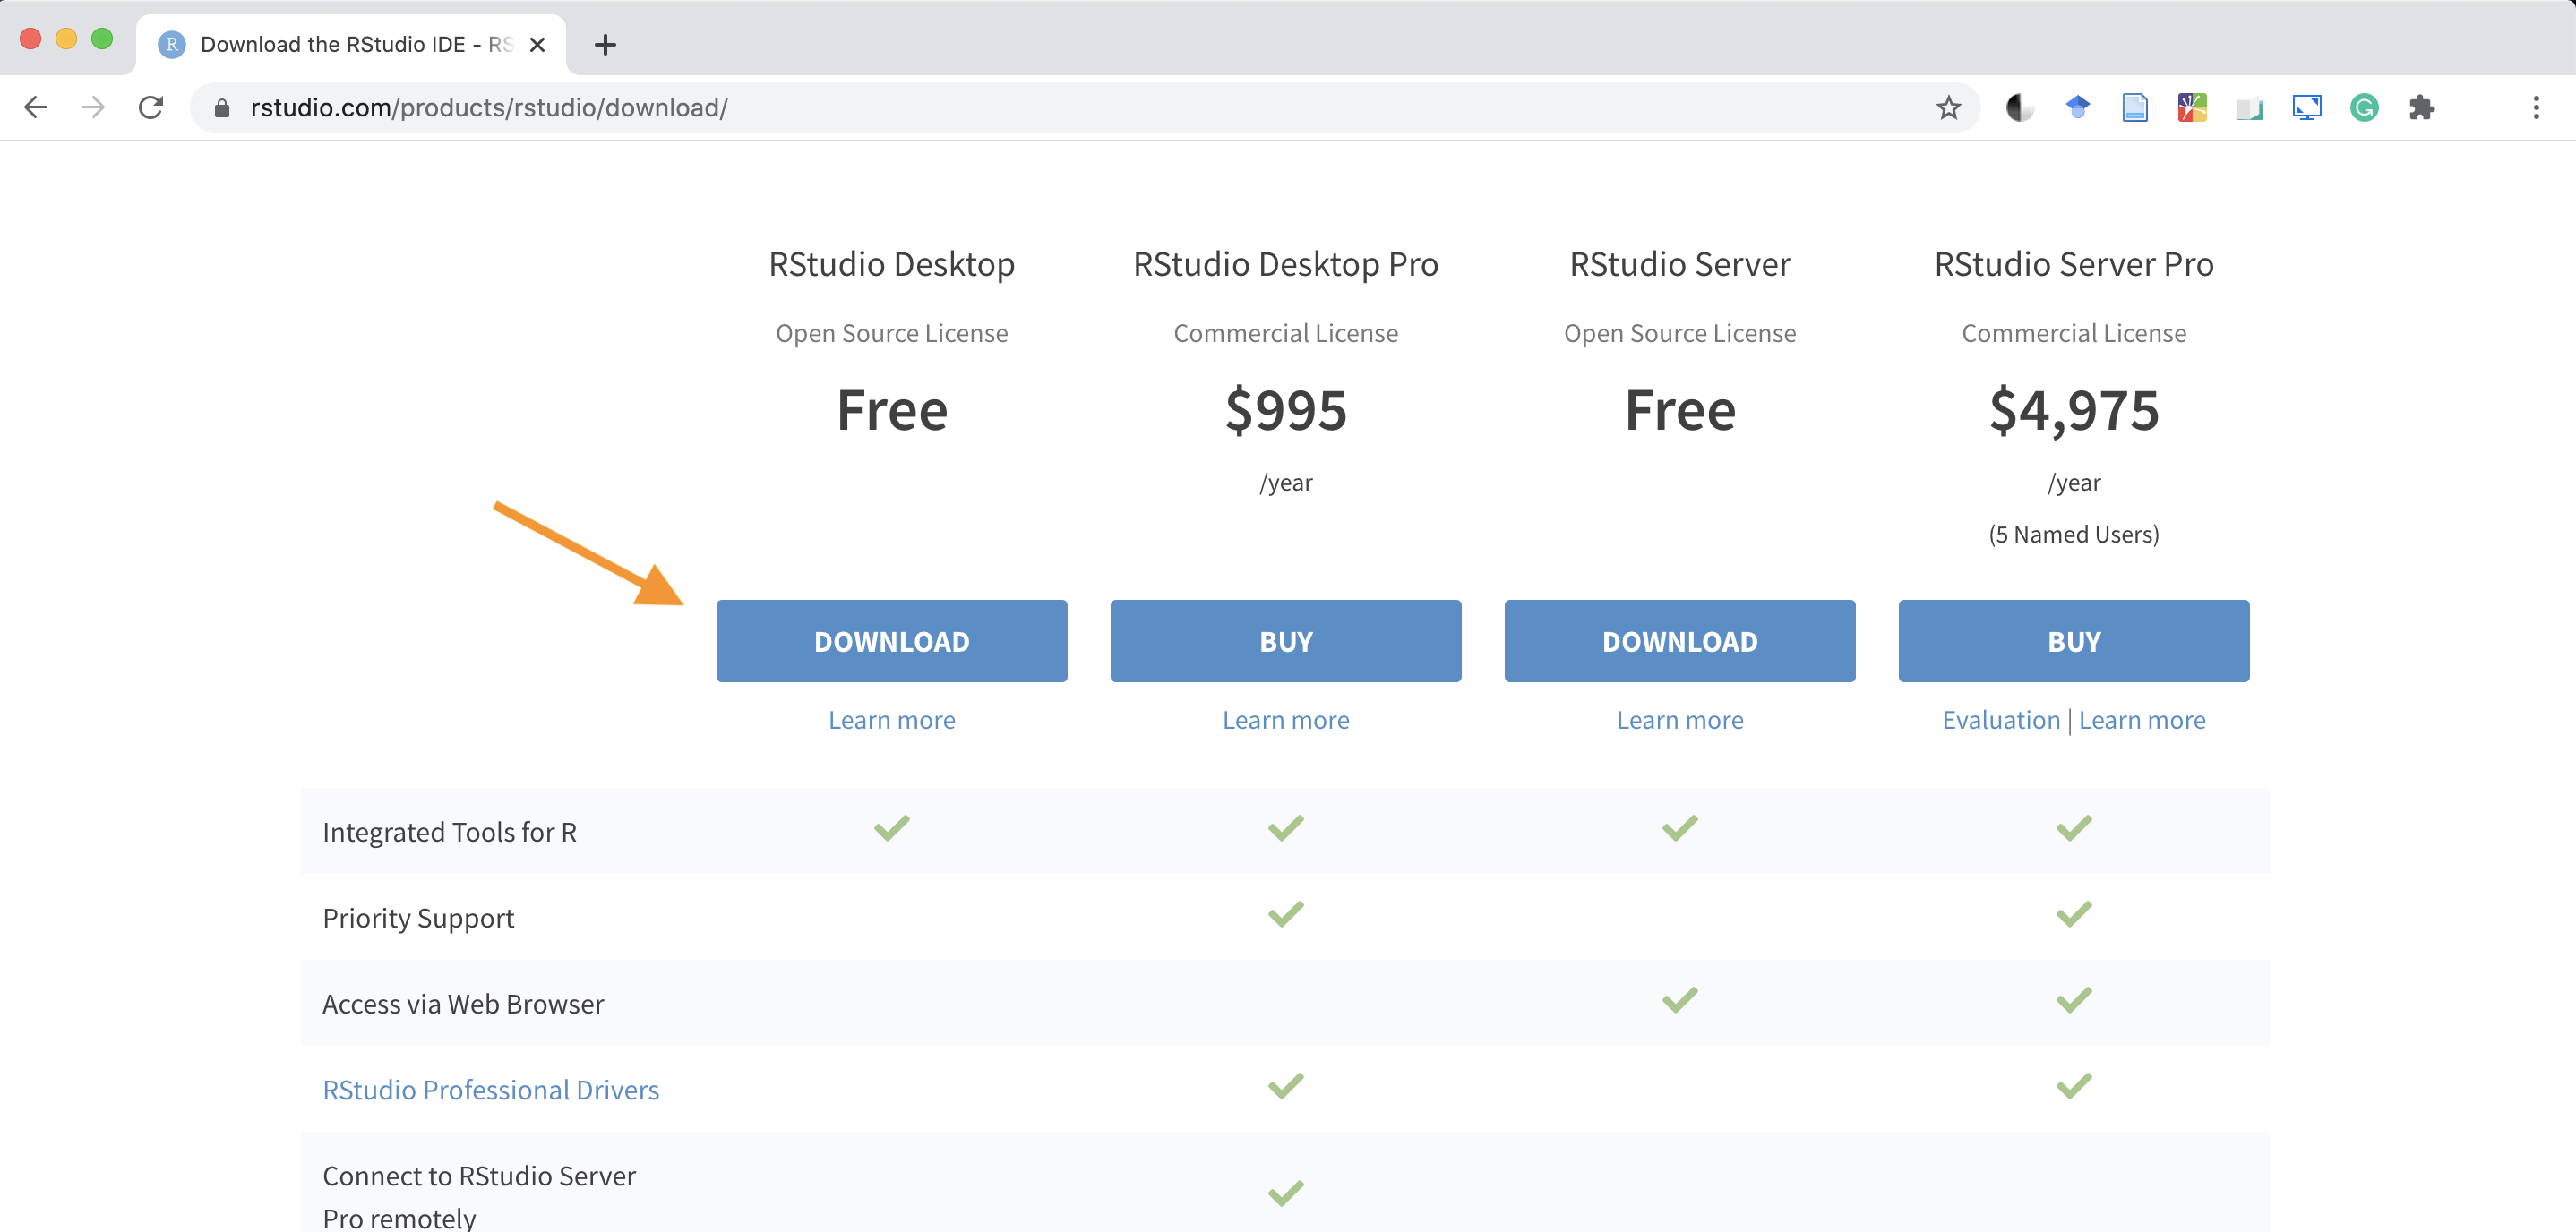
\includegraphics[width=0.95\textwidth,height=\textheight]{images/install_rstudio2.png}

\begin{enumerate}
\def\labelenumi{\arabic{enumi}.}
\setcounter{enumi}{3}
\tightlist
\item
  Selezionare la versione corretta a seconda del proprio sistema operativo
\end{enumerate}

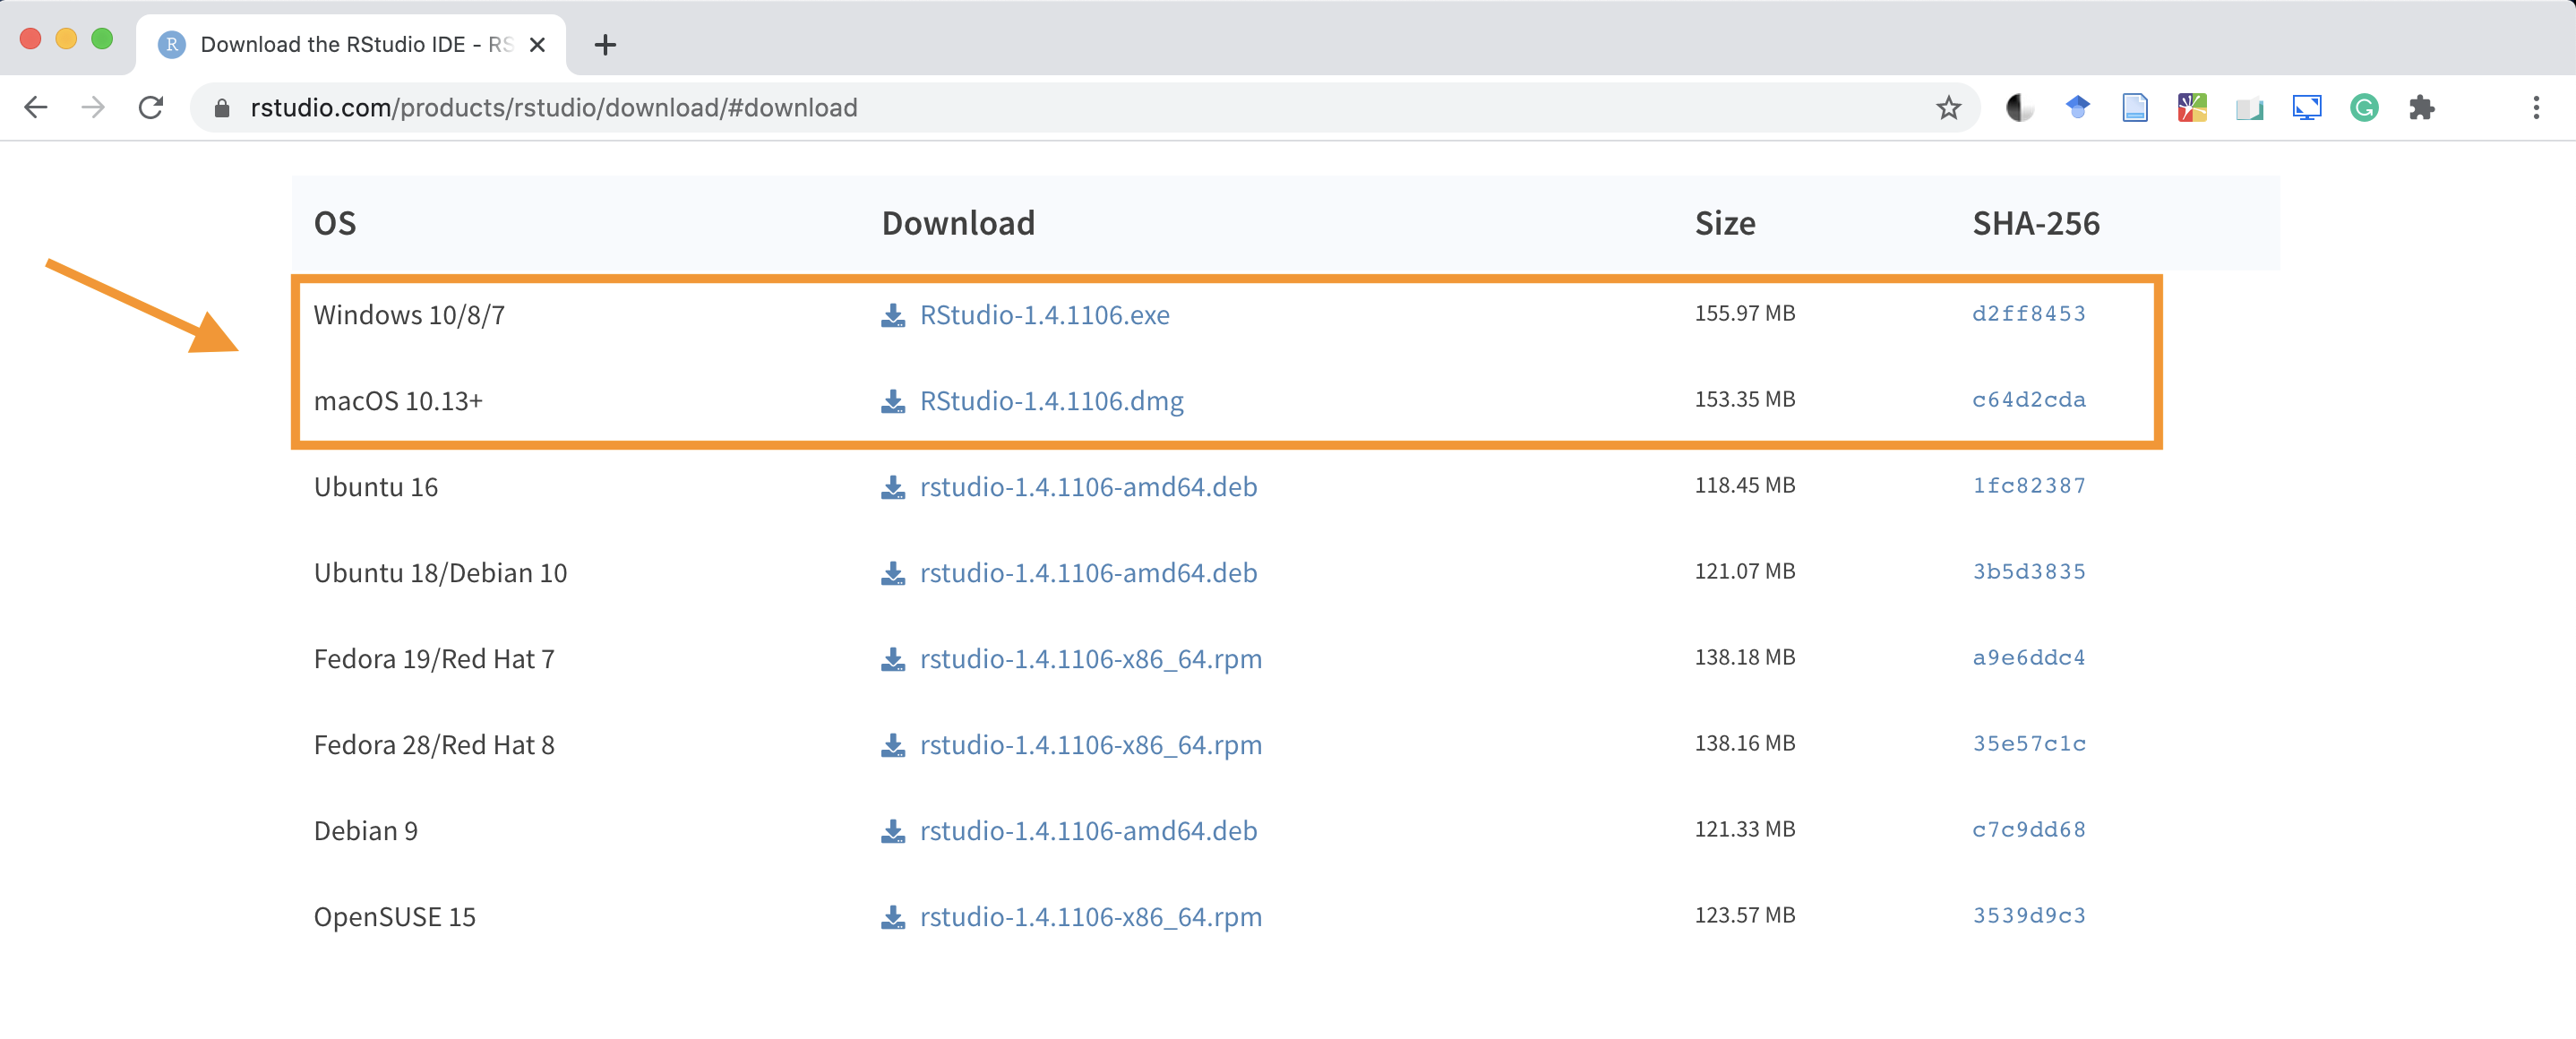
\includegraphics[width=0.95\textwidth,height=\textheight]{images/install_rstudio3.png}

\begin{enumerate}
\def\labelenumi{\arabic{enumi}.}
\setcounter{enumi}{4}
\tightlist
\item
  Al termine del download, eseguire il file e seguire le istruzioni fino al termine dell'installazione
\end{enumerate}

\hypertarget{r-studio-in-linux}{%
\subsection{R Studio in Linux}\label{r-studio-in-linux}}

In questo caso, come su Windows e MacOS l'installazione consiste nello scaricare ed eseguire il file corretto, in base alla distribuzione (ad esempio \texttt{.deb} per Ubuntu e derivate). Importante, nel caso di Ubuntu (ma dovrebbe valere anche per le altre distribuzioni) anche versioni successive a quella indicata (es. Ubuntu 16) sono perfettamente compatibili.

\hypertarget{rstudio-gui}{%
\chapter{Interfaccia RStudio}\label{rstudio-gui}}

In questo capitolo presenteremo l'interfaccia utente di RStudio. Molti aspetti che introdurremo brevemente qui verranno discussi nei sucessivi capitoli. Adesso ci interessa solo famigliarizzare con l'interfaccia del nostro strumento di lavoro principale ovvero RStudio.

Come abbiamo visto nel Capitolo \ref{install}, R è il vero ``motore computazionale'' che ci permette di compiere tutte le operazioni di calcolo, analisi statistiche e magie varie. Tuttavia l'interfaccia di base di R, definita \textbf{Console} (vedi Figura \ref{fig:r-console}), è per così dire \emph{démodé} o meglio, solo per veri intenditori.

\begin{figure}

{\centering 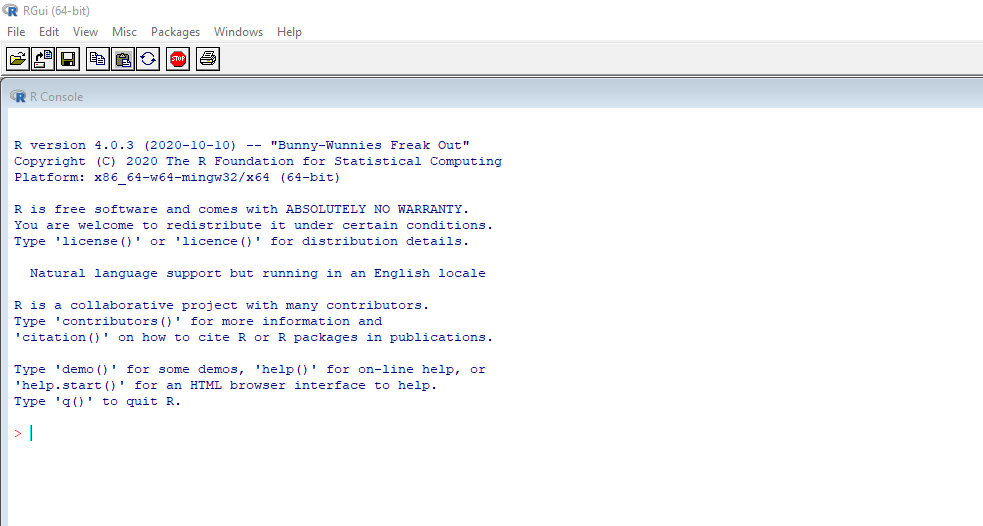
\includegraphics[width=0.85\linewidth]{images/r-console} 

}

\caption{La console di R, solo per veri intenditori}\label{fig:r-console}
\end{figure}

In genere, per lavorare con R viene utilizzato RStudio. RStudio è un programma (IDE - Integrated Development Environment) che integra in un unica interfaccia utente (GUI - Graphical User Interface) diversi strumenti utili per la scrittura ed esecuzione di codici. L'interfaccia di RStudio è costituita da 4 pannelli principali (vedi Figura \ref{fig:rstudio-gui}):

\begin{figure}

{\centering 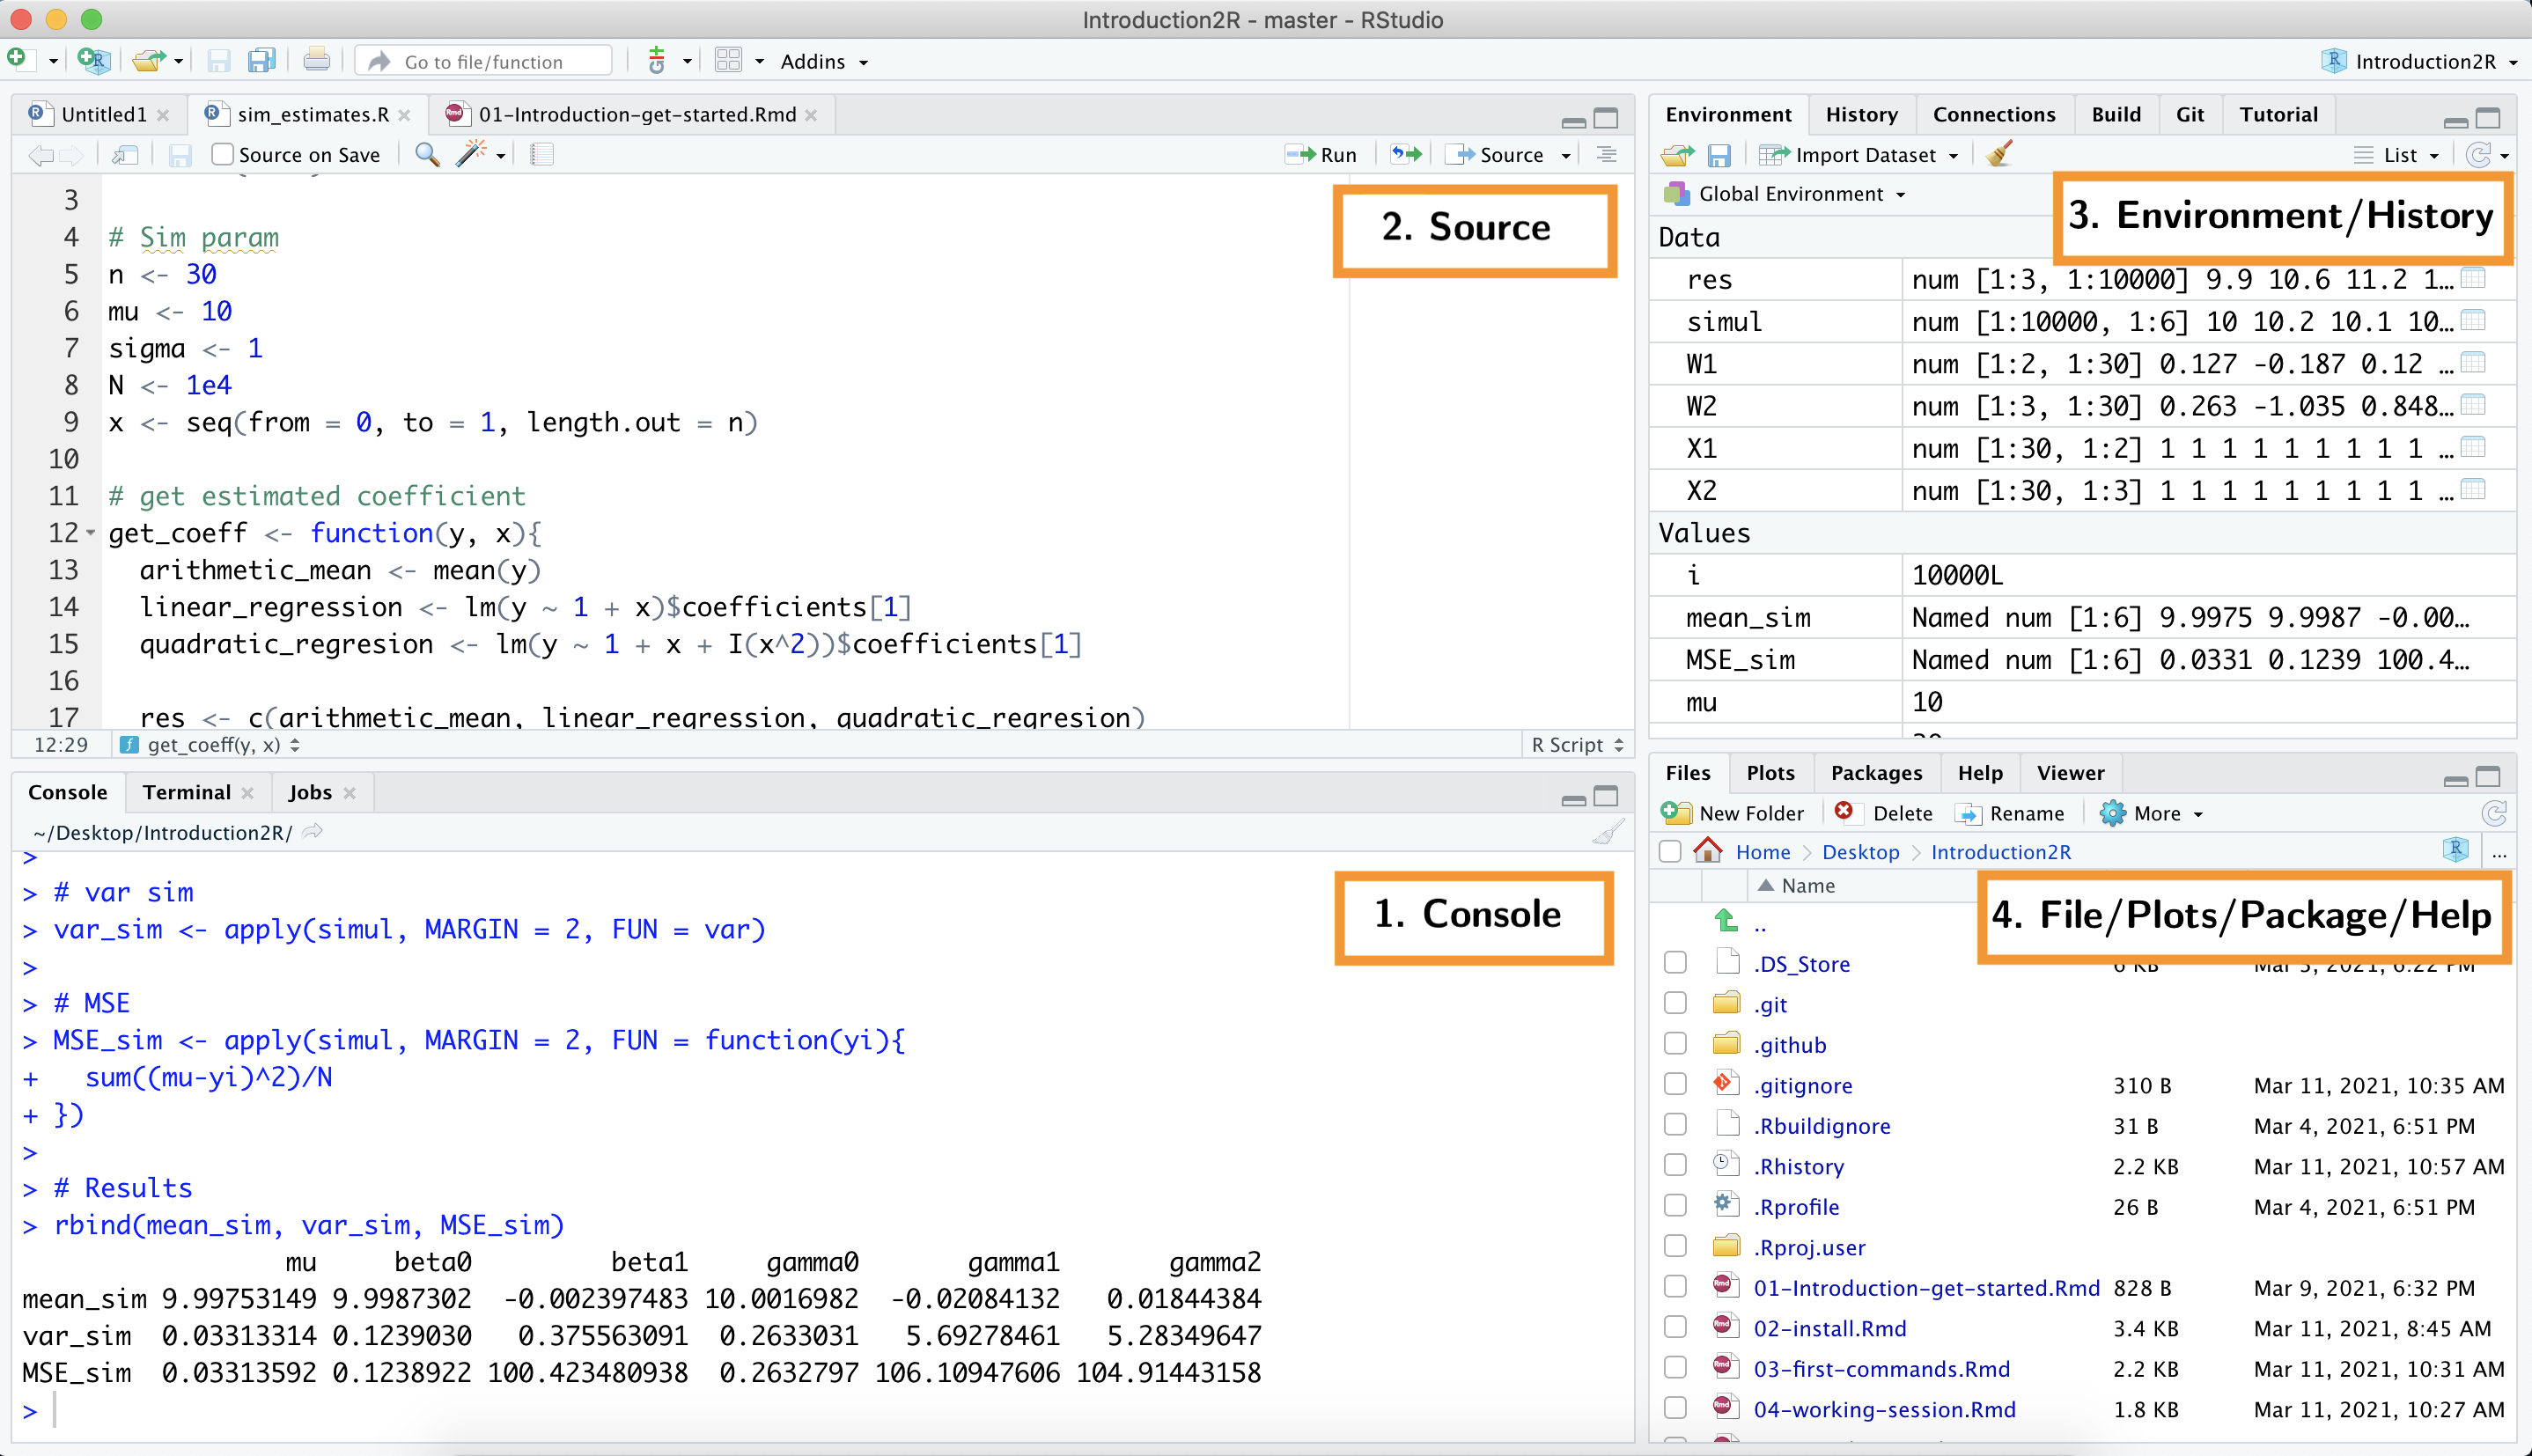
\includegraphics[width=0.85\linewidth]{images/rstudio-gui} 

}

\caption{Interfaccia utente di Rstudio con i suoi 4 pannelli}\label{fig:rstudio-gui}
\end{figure}

\hypertarget{console-il-cuore-di-r}{%
\subsubsection*{1. Console: il cuore di R}\label{console-il-cuore-di-r}}
\addcontentsline{toc}{subsubsection}{1. Console: il cuore di R}

Qui ritroviamo la \emph{Console} di R dove vengono effetivemente eseguiti tutti i tuoi codici e comandi. Nota come nell'ulitma riga della \emph{Console} appaia il carattere \texttt{\textgreater{}}. Questo è definito \emph{prompt} è ci indica che R in attesa di nuovi comandi da eseguire.

La \emph{Console} di R è un'interfaccia a linea di comando. A differenza di altri programmi ``\emph{punta e clicca}'', in R è necessario digitare i comandi utilizzando la tastiera. Per eseguire dei comandi possiamo direttamnte scrivere nella \emph{Console} le operazioni da eseguire e premere \texttt{invio}. R eseguirà immediatamente i nostro comando, riporterà il risultato e nella linea successiva apparirà nuovamente il \emph{prompt} indicando che R è pronto ad eseguire un altro comando (vedi Figura \ref{fig:comand-sequence}).

\begin{figure}

{\centering 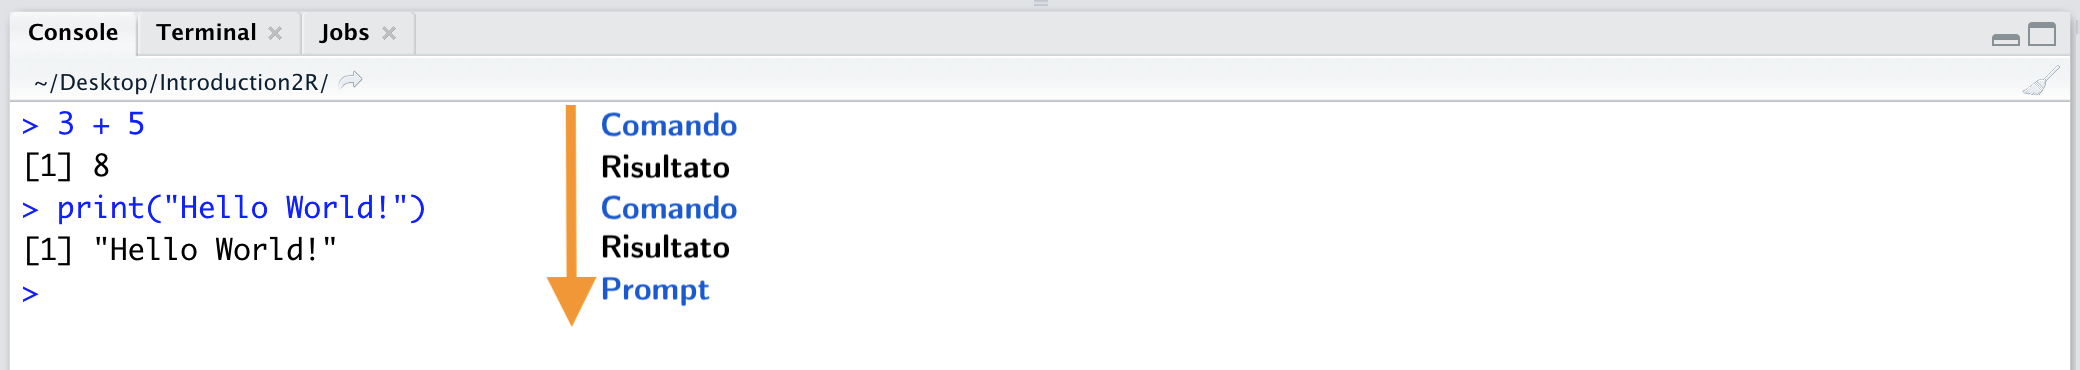
\includegraphics[width=0.95\linewidth]{images/comand-sequence} 

}

\caption{Esecuzione di comandi direttamente nella console}\label{fig:comand-sequence}
\end{figure}

Nel caso di comandi scritti su più righe, vedi l'esempio di Figura \ref{fig:multiple-line-comand}, è possibile notare come venga mostrato il simbolo \texttt{+} come \emph{prompt}. Questo indica che R è in attesa che l'intero comando venga digitato prima che esso venga eseguito.

\begin{figure}

{\centering 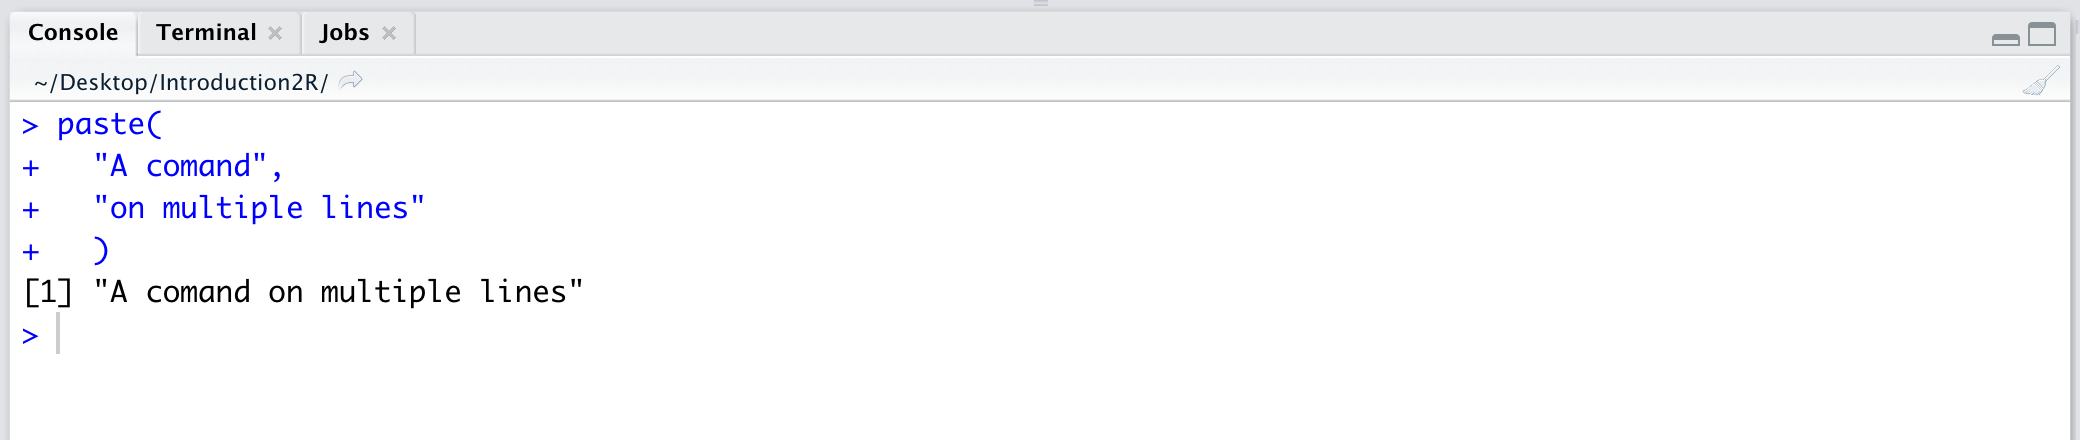
\includegraphics[width=0.95\linewidth]{images/multiple-line-comand} 

}

\caption{Esecuzione di un comando su più righe}\label{fig:multiple-line-comand}
\end{figure}

Come avrai notato facendo alcune prove, i comandi digitati nella \emph{Console} vengono eseguiti immediatamente ma non sono salvati. Per rieseguire un comando, possiamo navigare tra quelli precedentementemente eseguiti usando le freccie della tastiera \(\uparrow\downarrow\). Tuttavia, in caso di errori dovremmo riscrivere e rieseguire tutti i comandi. Siccome scrivere codici è un continuo ``\emph{try and error}'', lavorare unicamente dalla \emph{Console} diventa presto caotico. Abbiamo bisogno quindi di una soluzione che ci permetta di lavrorare più comodamente sui nostri codici e di poter salvare i nostri comandi da eseguire all'occorrenza con il giusto ordine. La soluzione sono gli \emph{Scripts} che introdurremo vedremo nella prossima sezione.

\begin{tip}[Interrompere un comando]

Potrebbe accadere che per qualche errore nel digitare un comando o perchè sono richiesti lunghi tempi computazionali, la \emph{Console} di R diventi non responsiva. In questo caso è necessario interrompere la scrittura o l'esecuzione di un comando. Vediamo due situazioni comuni:

\begin{enumerate}
\def\labelenumi{\arabic{enumi}.}
\tightlist
\item
  \textbf{Continua a comparire il prompt} \texttt{+}. Specialmente nel caso di utilizzo di parentesi e lunghi comandi, accade che una volta premuto \texttt{invio} R non esegua alcun comando ma resta in attesa mostrando il \emph{prompt} \texttt{+} (vedi Figure seguente). Questo è in genere dato da un errore nella sintassi del comando (e.g., un errore nell'uso delle parentesi o delle virgole). Per riprendere la sessione è necessario premere il tasto \texttt{esc} della tastiera. L'apprire del \emph{prompt} \texttt{\textgreater{}}, indica che R è nuovamente in ascolto pronto per esequire un nuovo comando ma attento a non ripetere lo stesso errore, la sintassi dei comandi è importante (vedi Capitolo TODO).
\end{enumerate}

\begin{center}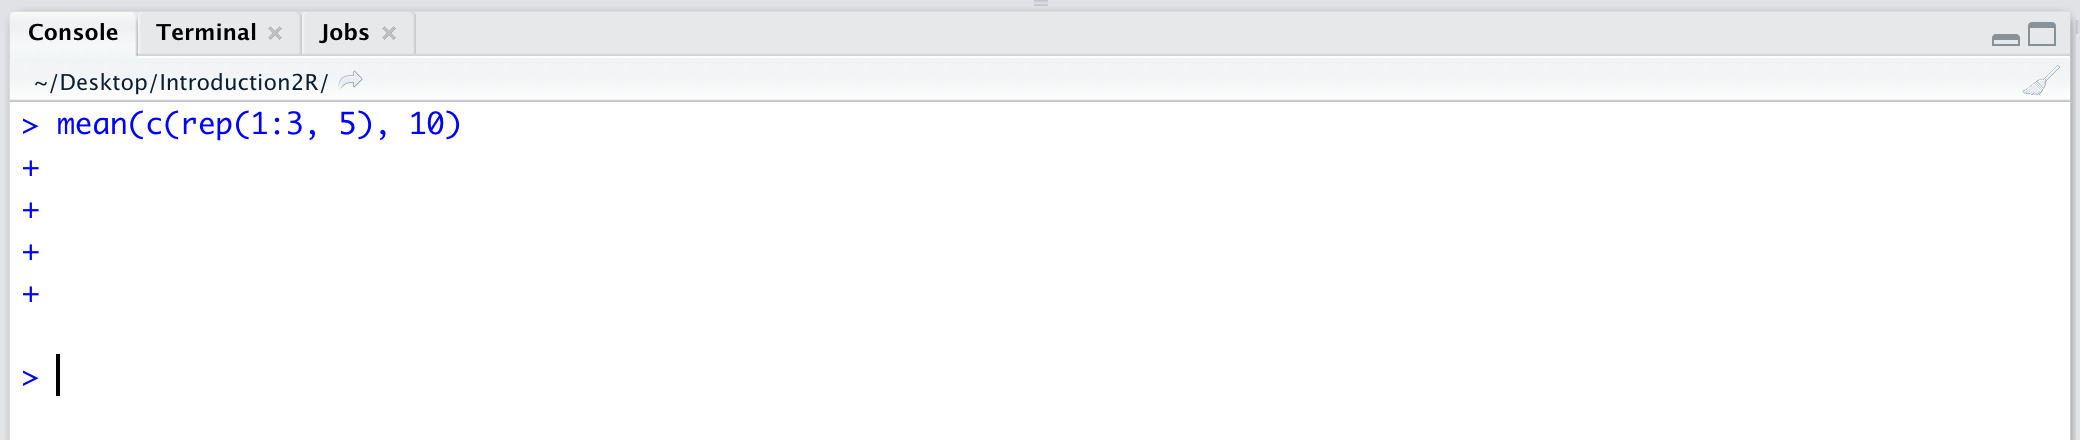
\includegraphics[width=0.95\linewidth]{images/comand-esc} \end{center}

\begin{enumerate}
\def\labelenumi{\arabic{enumi}.}
\setcounter{enumi}{1}
\tightlist
\item
  \textbf{R non risponde}. Alcuni calcoli potrebbero richiedere molto tempo o semplicemnte un qualche problema ha mandato in loop la tua sessione di lavoro. In questa situazione la \emph{Console} di R diventa non responsiva. Nel caso fosse necessario interrompere i processi attualmente in esecuzione devi premere il pulsante \emph{STOP} come indicato nella Figura seguente. R si fermerà e ritornerà in attesa di nuovi comandi (\emph{prompt} \texttt{\textgreater{}}).
\end{enumerate}

\begin{center}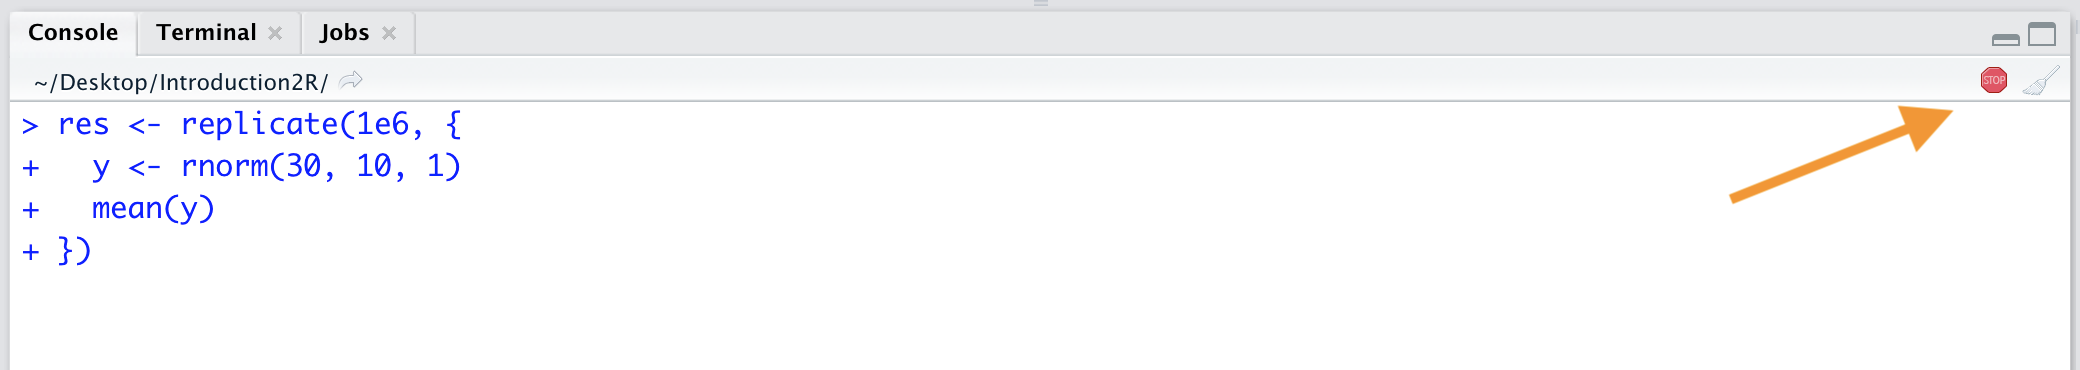
\includegraphics[width=0.95\linewidth]{images/console-stop} \end{center}

\end{tip}

\begin{trick}[Force Quit]

In alcuni casi estremi in cui R sembra non rispondere, usa i comandi \texttt{Ctrl-C} per forzare R a interrompere il processo in esecuzione.

Come ultima soluzione ricorda uno dei principi base dell'informatica ``\emph{spegni e riaccendi}'' (a volte potrebbe bastare chiudere e riaprire RStudio).

\end{trick}

\hypertarget{source-il-tuo-blocco-appunti}{%
\subsubsection*{2. Source: il tuo blocco appunti}\label{source-il-tuo-blocco-appunti}}
\addcontentsline{toc}{subsubsection}{2. Source: il tuo blocco appunti}

In questa parte vengono mostrati i tuoi \emph{Scripts}. Questi non sono altro che degli speciali documenti (con estensione ``\textbf{.R}'') in cui sono salvati i tuoi codici e comandi che potrai eseguire quando necessario in R. Gli \emph{Scripts} ti permetteranno di lavorare comodamente sui tuoi codici, scrivere i comandi, corregerli, organizzarli, aggiungere dei commenti e soprattutto salvarli.

Dopo aver terminato di scrivere i comandi, posiziona il cursore sulla stessa linea del comando che desideri eseguire e premi \texttt{command\ +\ invio} (MacOs) o \texttt{Ctrl+R} (Windows). Automaticamente il comando verà copiato nella \emph{Console} ed eseguito. In alternativa potrai premere il tasto \textbf{Run} indicato dalla freccia in Figura \ref{fig:script-run}.

\begin{figure}

{\centering 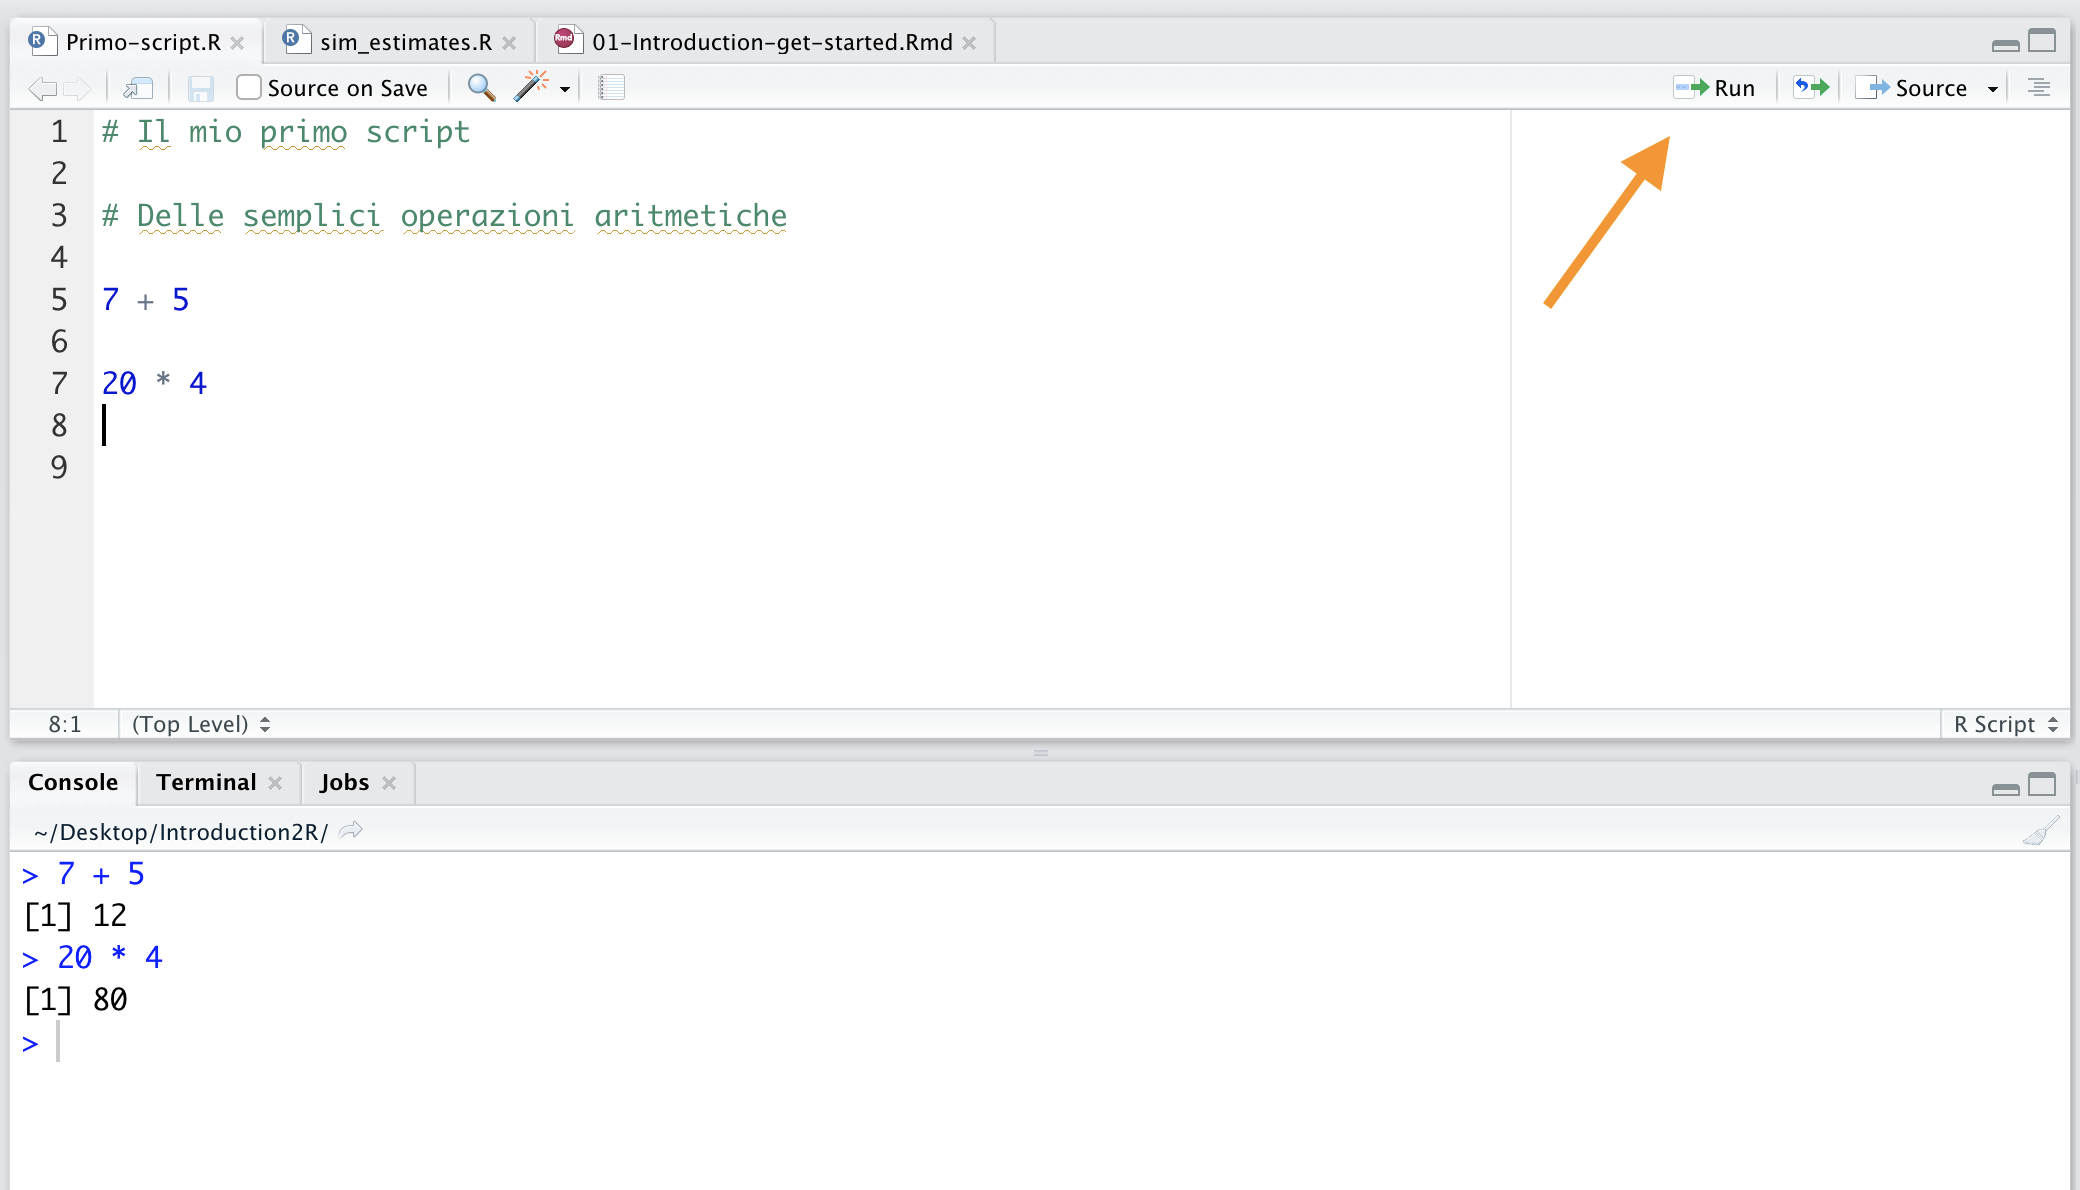
\includegraphics[width=0.95\linewidth]{images/script-run} 

}

\caption{Esecuzione di un comando da script premi `command + invio` (MacOs)/ `Ctrl+R` (Windows) o premi il tasto indicato dalla freccia}\label{fig:script-run}
\end{figure}

\begin{tip}[Commenti]

Se hai guardato con attenzione lo script rappresentato in Figura \ref{fig:script-run}, potresti aver notato delle righe di testo verde precedute dal simbolo \texttt{\#}. Questo simbolo può essere utlizzato per inserire dei \emph{commenti} all'interno dello script. R ignorerà qualsiasi commento ed eseguirà soltato le parti di codici.

L'utilizzo dei commenti è molto importante nel caso di script complessi poichè ci permette di spiegare e documentare il codice che viene eseguito. Nel Capitolo TODO approfondiremo il loro utilizzo.

\end{tip}

\hypertarget{environment-e-history-la-sessione-di-lavoro}{%
\subsubsection*{3. Environment e History: la sessione di lavoro}\label{environment-e-history-la-sessione-di-lavoro}}
\addcontentsline{toc}{subsubsection}{3. Environment e History: la sessione di lavoro}

Qui sono presentati una serie di pannelli utili per valutare informazioni inerenti alla propria sessione di lavoro. I pannelli principali sono \emph{Environment} e \emph{History} (gli altri pannelli presenti in Figura \ref{fig:environment} riguardanno funzioni avanzate di RStudio).

\begin{itemize}
\tightlist
\item
  \textbf{Environment}: elenco tutti gli oggetti e variabili attualmente presenti nel'ambiente di lavoro. Approfondiremo i concetti di variabili e di ambiente di lavoro rispettivamente nel Capitolo \ref{objects-functions} e Capitolo TODO.
\end{itemize}

\begin{figure}

{\centering 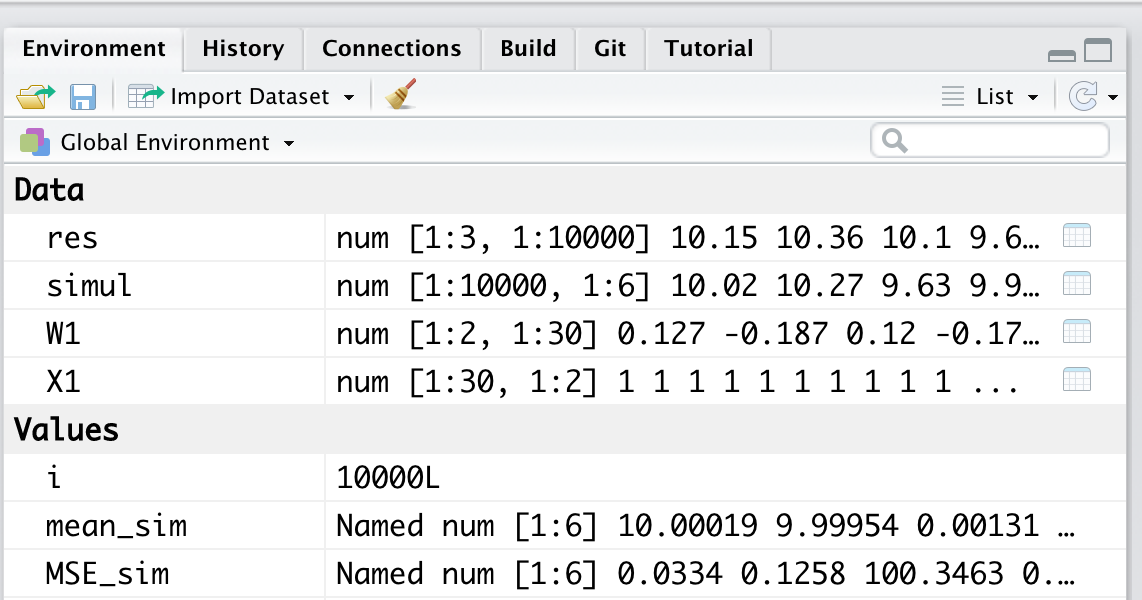
\includegraphics[width=0.6\linewidth]{images/environment} 

}

\caption{*Environment* - Elenco degli oggetti e variabili presenti nel'ambiente di lavoro}\label{fig:environment}
\end{figure}

\begin{itemize}
\tightlist
\item
  \textbf{History}: elenco di tutti i comandi precedentemente eseguiti nella console. Nota che questo no equivale ad uno script, anzi, è semplicemente un elenco non modificabile (e quasi mai usato).
\end{itemize}

\hypertarget{file-plots-package-help-system-management}{%
\subsubsection*{4. File, Plots, Package, Help: system management}\label{file-plots-package-help-system-management}}
\addcontentsline{toc}{subsubsection}{4. File, Plots, Package, Help: system management}

In questa parte sono raccolti una serie di pannelli utilizzatti per interfacciarsi con ulteriori risorse del sistema (e.g., file e pacchetti) o produrre output quali grafici e tabelle.

\begin{itemize}
\tightlist
\item
  \textbf{Files}: pannello da cui è possibile navigare tra tutti i file del proprio computer
\end{itemize}

\begin{figure}

{\centering 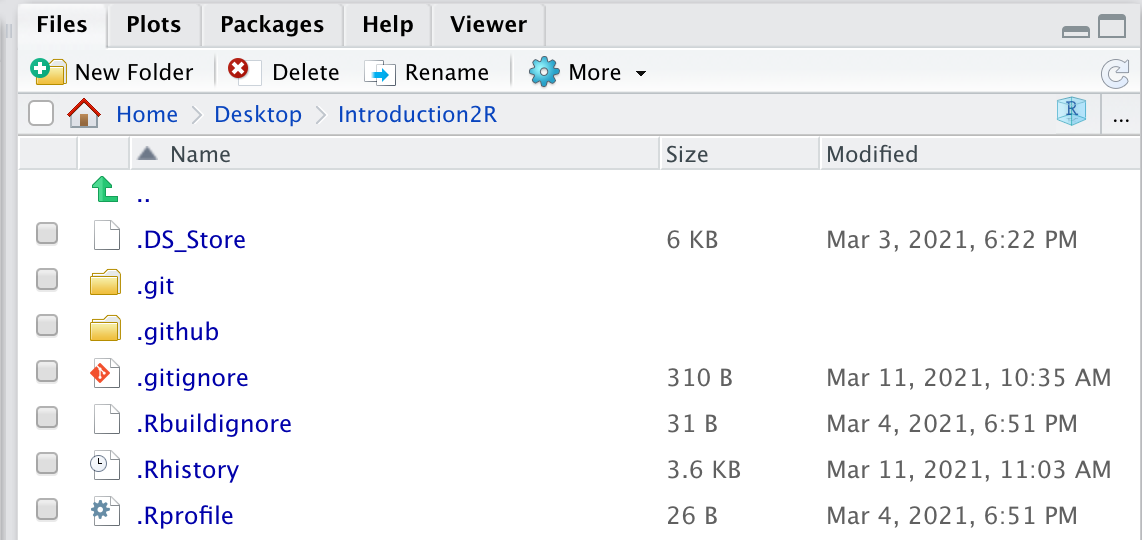
\includegraphics[width=0.6\linewidth]{images/files} 

}

\caption{*Files* - permette di navigare tra i file del proprio computer}\label{fig:files}
\end{figure}

\begin{itemize}
\tightlist
\item
  \textbf{Plots}: pannello i cui vengono prodotti i grafici e che è possibil esportare cliccando \emph{Export}.
\end{itemize}

\begin{figure}

{\centering 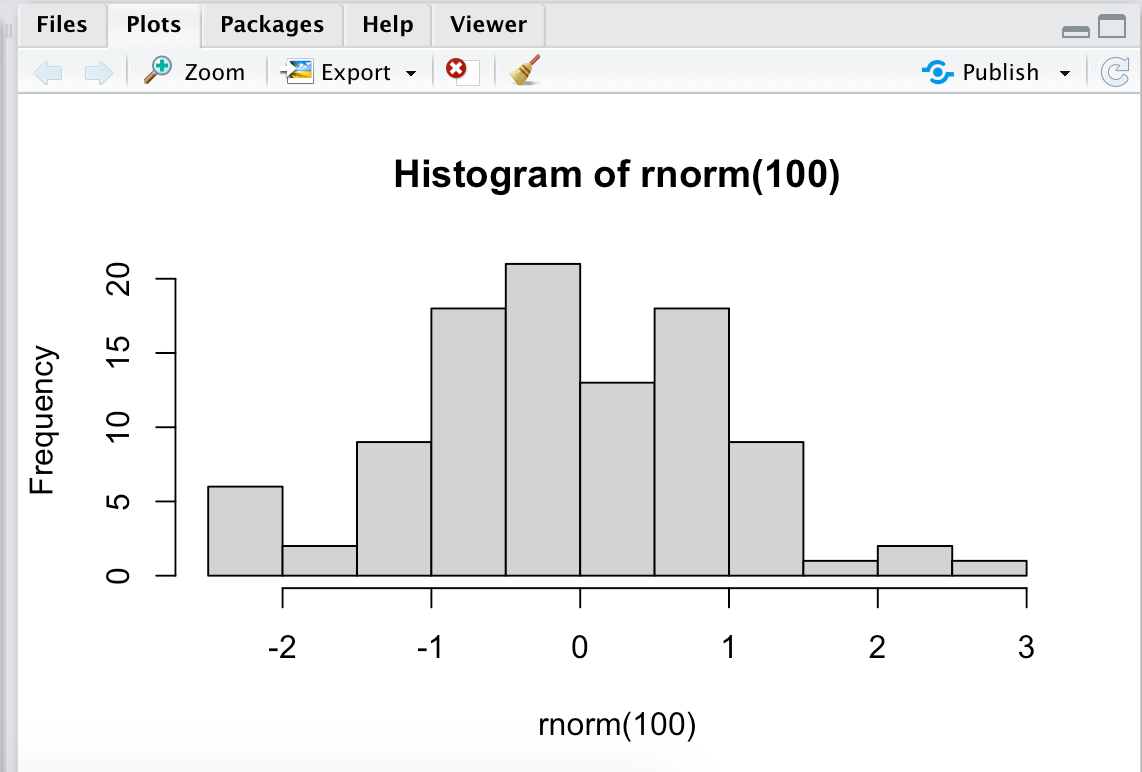
\includegraphics[width=0.6\linewidth]{images/plots} 

}

\caption{*Plots* - presentazione dei grafici}\label{fig:plots}
\end{figure}

\begin{itemize}
\tightlist
\item
  \textbf{Packages}: elenco dei pacchetti di R (questo argomento verrà approfondito nel Capitolo TODO).
\end{itemize}

\begin{figure}

{\centering 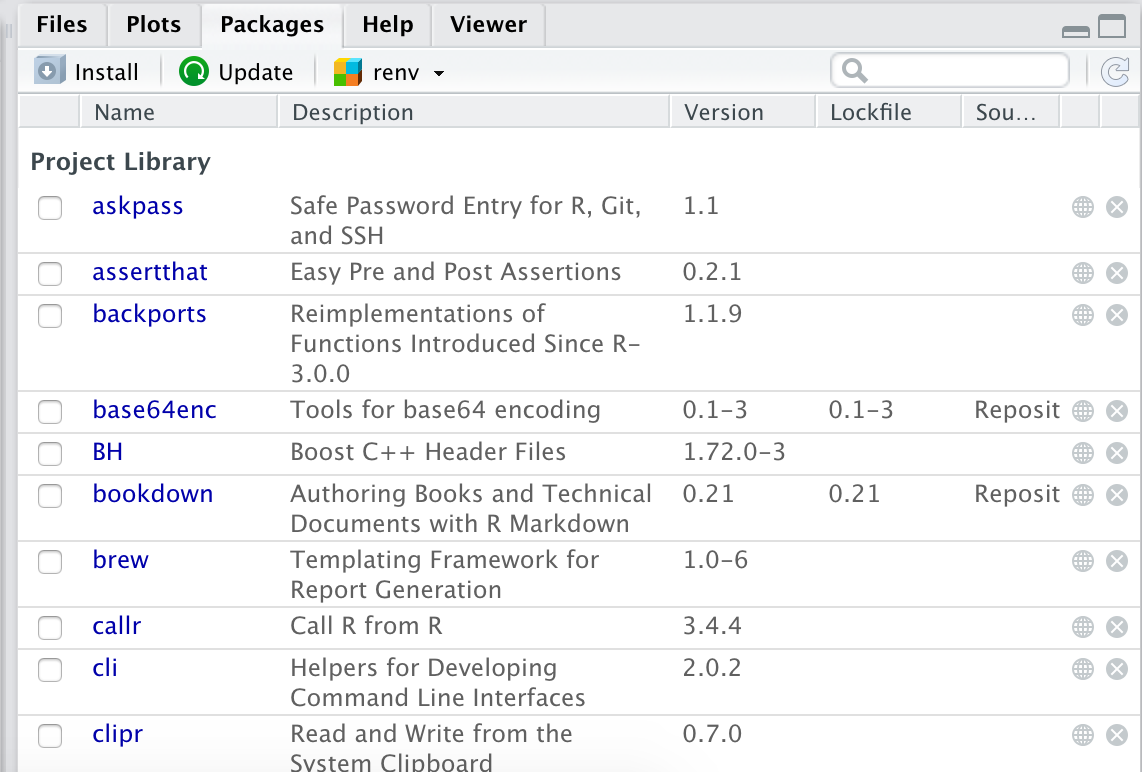
\includegraphics[width=0.6\linewidth]{images/packages} 

}

\caption{*Packages* - elenco dei pacchetti di R}\label{fig:packages}
\end{figure}

\begin{itemize}
\tightlist
\item
  \textbf{Help}: utilizzato per navigare la documentazione interna di R (questo argomento verrà approfondito nel Capitolo TODO).
\end{itemize}

\begin{figure}

{\centering 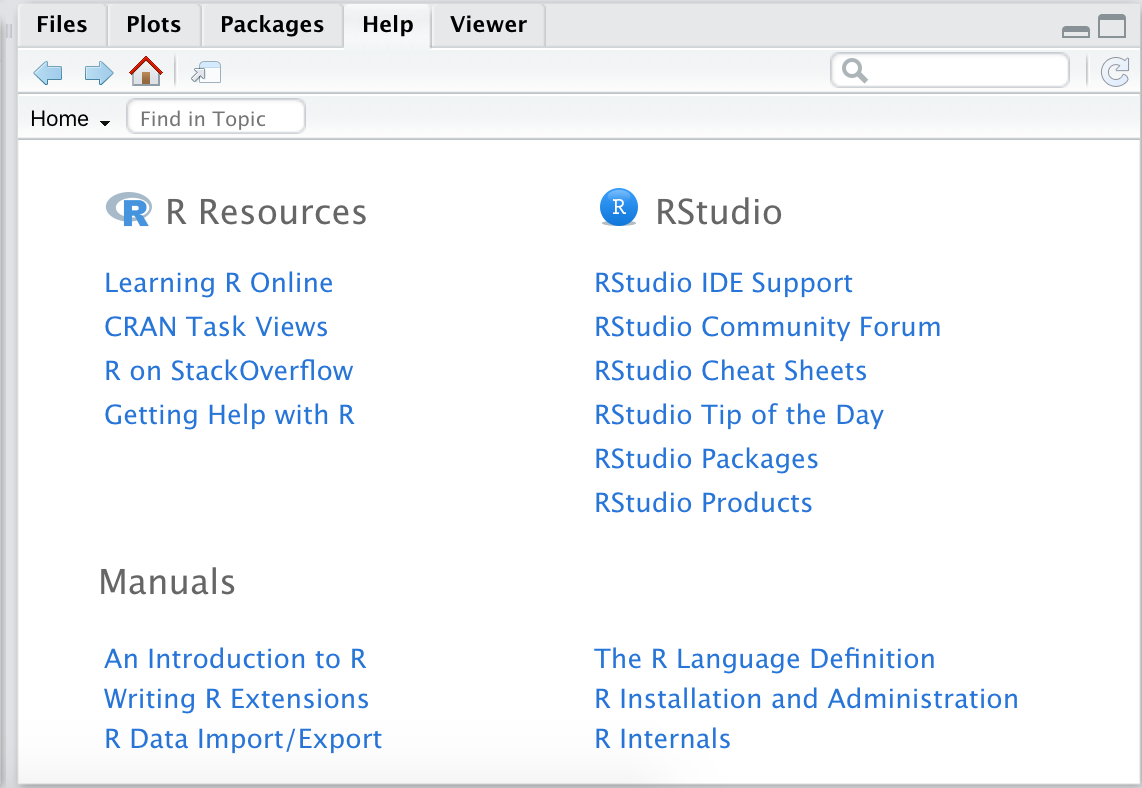
\includegraphics[width=0.6\linewidth]{images/help} 

}

\caption{*Help* -  documentazione di R}\label{fig:help}
\end{figure}

\begin{tip}[Personalizza tema e layout]

RStudio permette un ampio grado di personalizzazione dell'intrafaccia grafica utilizzata. E' possibile cambiare tema, font e disposizione dei pannelli a seconda dei tuoi gusti ed esigenze.

Prova a cambiare il tema dell editor in \emph{Idle Fingers} per utlizzare on background scuro che affatichi meno la vista (vedi Figura seguente). Clicca su RStudio \textgreater{} Preferenze \textgreater{} Appearence (MacOS) o Tools \textgreater{} Options \textgreater{} Appearence (Windows).

\begin{center}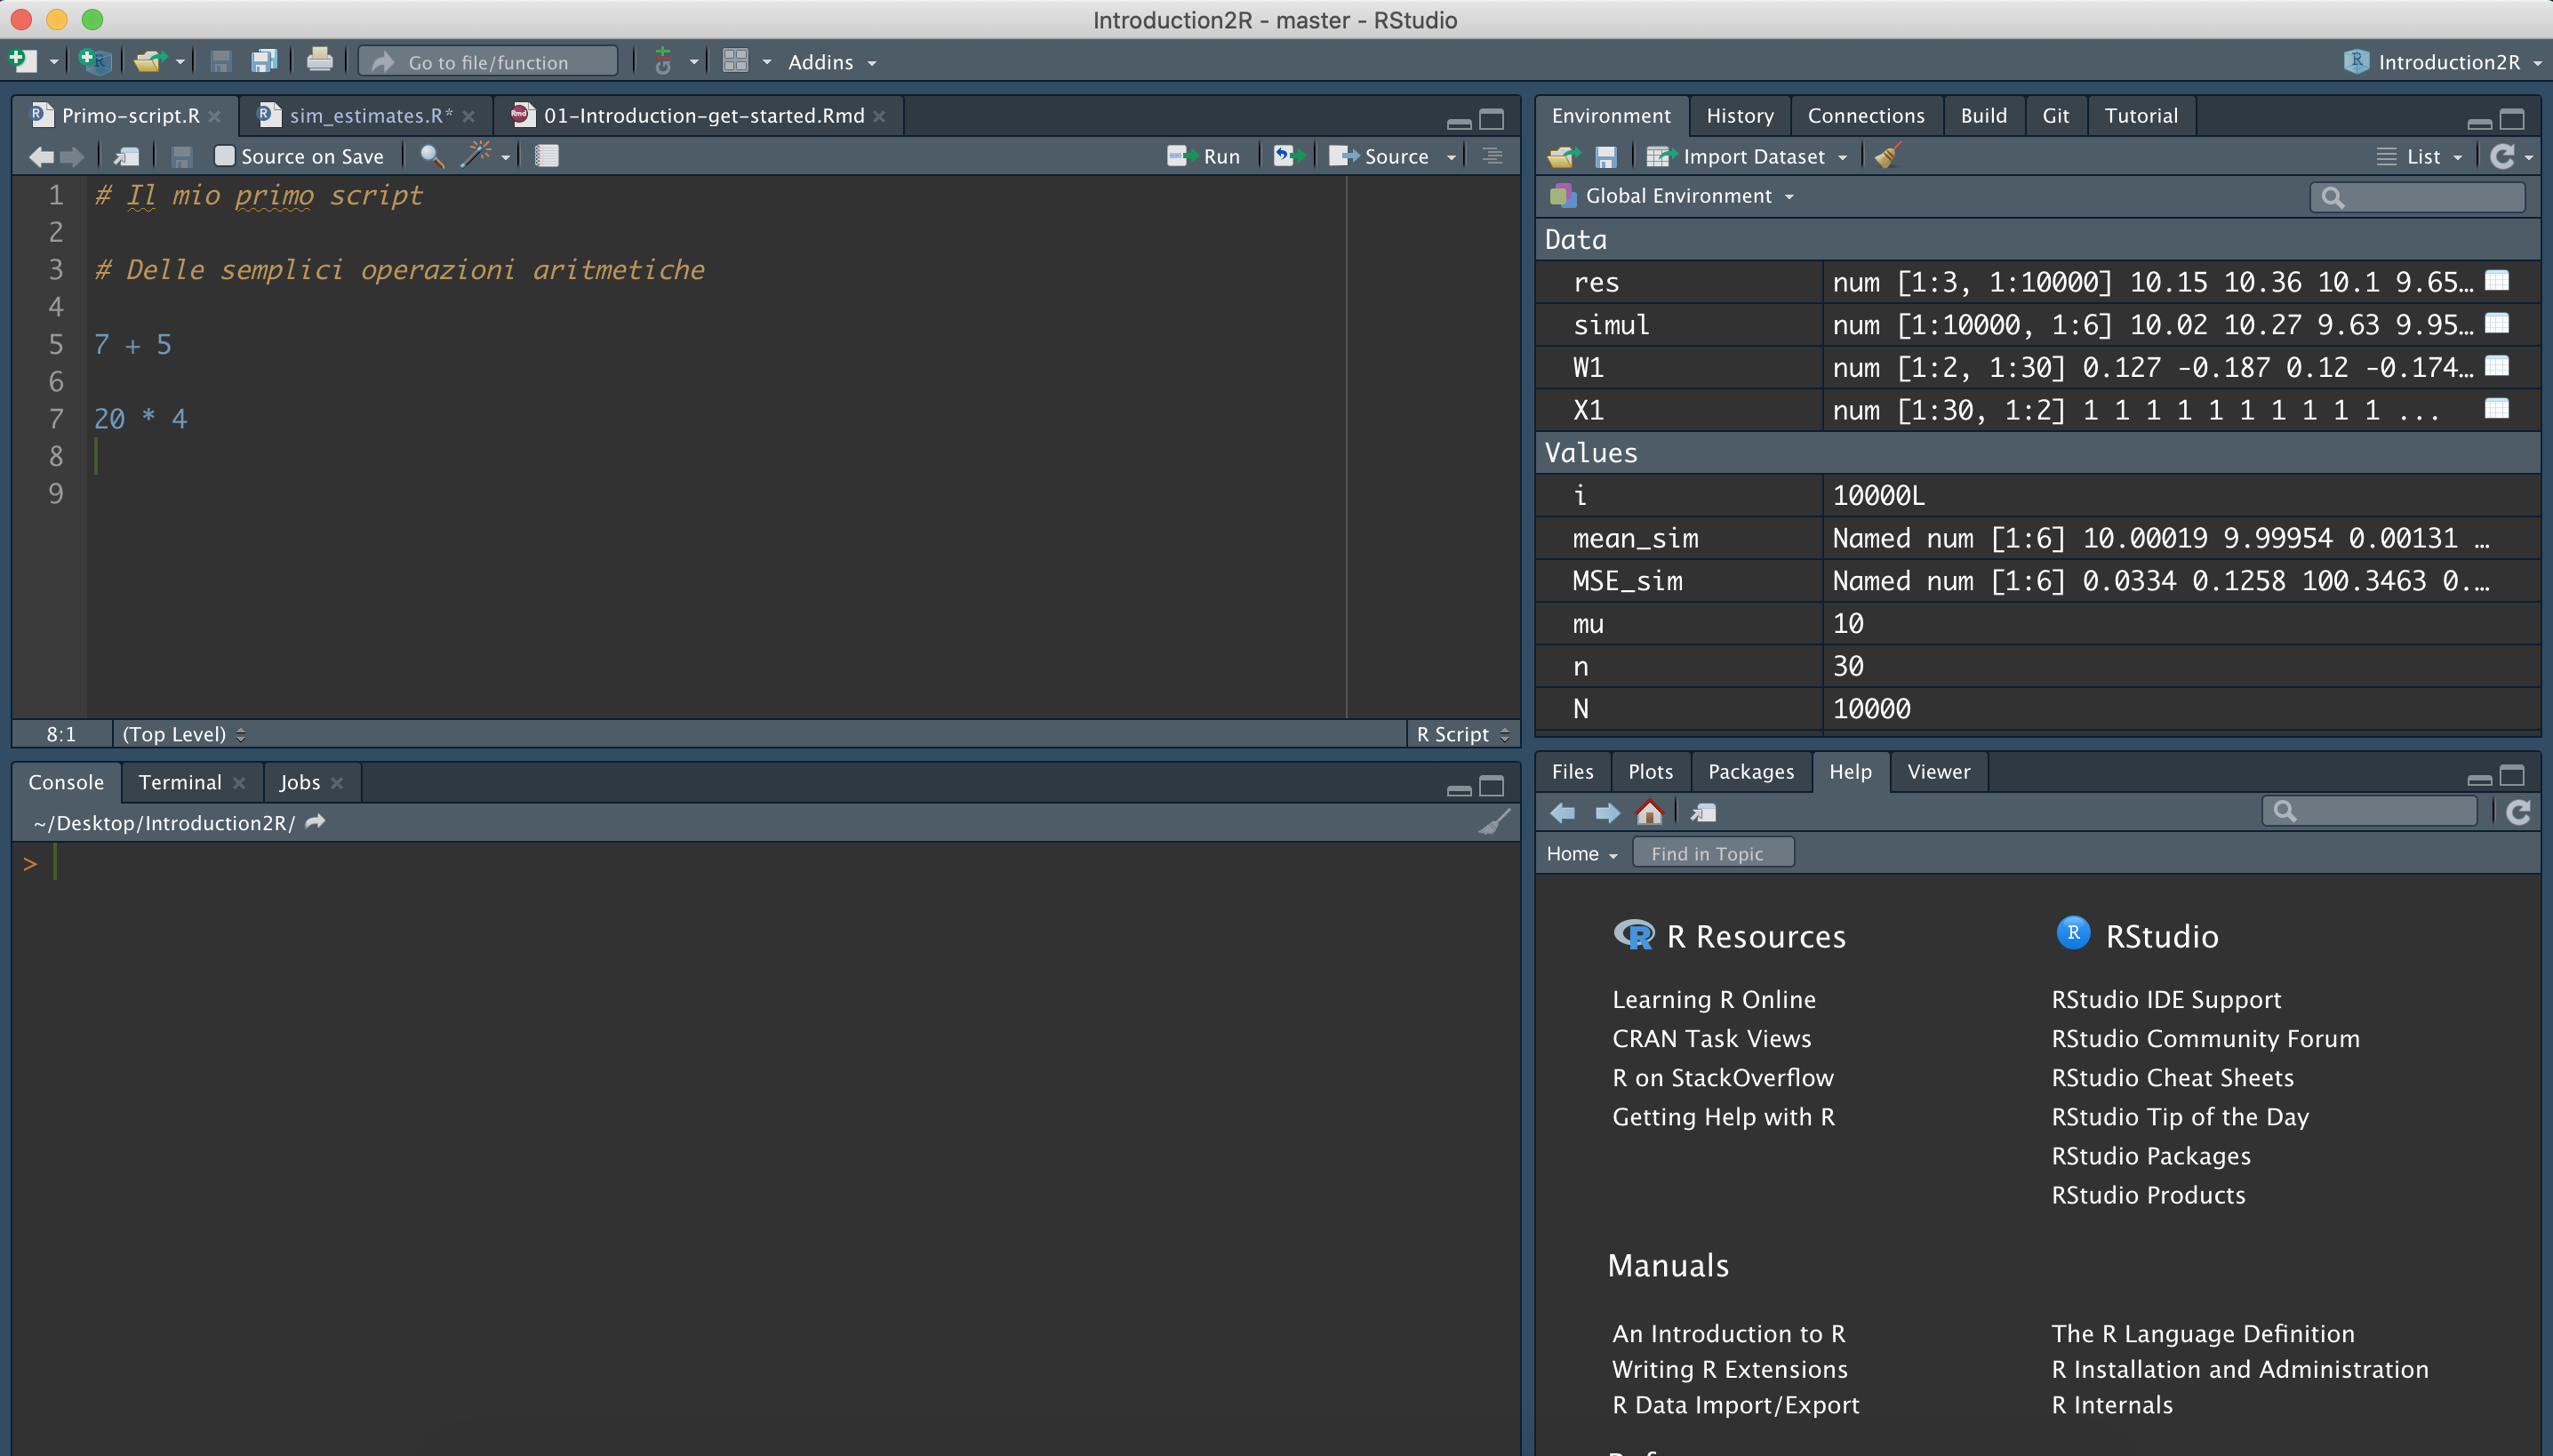
\includegraphics[width=0.9\linewidth]{images/dark-theme} \end{center}

\end{tip}

\hypertarget{first-comands}{%
\chapter{Primi Passi in R}\label{first-comands}}

Ora che abbiamo iniziato a famigliarizzare con il nostro stumento di lavoro possiamo finalmente dare fuoco alle polveri e concentraci sulla scrittura di codici!

In questo capitolo muoveremo i primi passi in R. Inizieremo vedendo come utilizzare operatori matematici, relazionali e logici per compiere semplici operazioni in R. Imparare R è un lungo percorso (scoop: questo percorso non termina mai dato che R è sempre in continuo sviiluppo). Soprattutto all'inizio può sembrare eccessivamente difficile poichè è si incontrano per la prima volta molti comandi e concetti di programmazione. Tuttavia, una volta famigliarizzato con gli apetti di base, la progressione diventa sempre più veloce (inarrestabile direi!).

In questo capitolo introdurremo per la prima volta molti elementi che saranno poi ripresi e approfonditi nei seguenti capitoli. Quindi non preoccuparti se non tutto ti sarà chiaro fin da subito. Imparare il tuo primo linguaggio di programmazione è difficile ma da qualche parte bisogna pure iniziare. Pronto per le tue prime linee di codice? Let's become a useR!

\hypertarget{math-operators}{%
\section{Operatori Matematici}\label{math-operators}}

R è un'ottima calcolatrice. Nella Tabella \ref{tab:table-math-operators} sono elencati i principali operatori matematici e funzioni usate in R.

\begin{table}[!h]

\caption{\label{tab:table-math-operators}Operatori Matematici}
\centering
\begin{tabular}[t]{l|l|l}
\hline
Funzione & Nome & Esempio\\
\hline
\texttt{x + y} & Addizione & \texttt{\makecell[l]{> 5 + 3 \\{[1]} 8}}\\
\hline
\texttt{x - y} & Sottrazione & \texttt{\makecell[l]{> 7 - 2 \\{[1]} 5}}\\
\hline
\texttt{x * y} & Moltiplicazione & \texttt{\makecell[l]{> 4 * 3 \\{[1]} 12}}\\
\hline
\texttt{x / y} & Divisione & \texttt{\makecell[l]{> 8 / 3 \\{[1]} 2.666667}}\\
\hline
\texttt{x \%\% y} & Resto della divisione & \texttt{\makecell[l]{> 7 \%\% 5 \\{[1]} 2}}\\
\hline
\texttt{x \%/\% y} & Divisione intera & \texttt{\makecell[l]{> 7 \%/\% 5 \\{[1]} 1}}\\
\hline
\texttt{x \^{} y} & Potenza & \texttt{\makecell[l]{> 3\^{}3 \\{[1]} 27}}\\
\hline
\texttt{abs(x)} & Valore assoluto & \texttt{\makecell[l]{> abs(3-5\^{}2) \\{[1]} 22}}\\
\hline
\texttt{sign(x)} & Segno di un'espressione & \texttt{\makecell[l]{> sign(-8) \\{[1]} -1}}\\
\hline
\texttt{sqrt(x)} & Radice quadrata & \texttt{\makecell[l]{> sqrt(25) \\{[1]} 5}}\\
\hline
\texttt{log(x)} & Logaritmo naturale & \texttt{\makecell[l]{> log(10) \\{[1]} 2.302585}}\\
\hline
\texttt{exp(x)} & Esponenziale & \texttt{\makecell[l]{> exp(1) \\{[1]} 2.718282}}\\
\hline
\texttt{\makecell[l]{sin(x)\\cos(x)\\tan(x)\\asin(x)\\acos(x)\\atan(x)}} & Funzioni trigonometriche & \texttt{\makecell[l]{ >sin(pi/2) \\{[1]}1 \\>cos(pi/2) \\{[1]}6.123234e-17}}\\
\hline
\texttt{factorial(x)} & Fattoriale & \texttt{\makecell[l]{> factorial(6) \\{[1]} 720}}\\
\hline
\texttt{choose(n, k)} & Coefficiente binomiale & \texttt{\makecell[l]{> choose(5,3) \\{[1]} 10}}\\
\hline
\end{tabular}
\end{table}

\begin{tip}[Le prime funzioni]

Nota come per svolgere operazioni come la radice quadrata o il valore assoluto vengono utlizzate delle specifiche funzioni. In R le funzioni sono richiamate digitando \texttt{\textless{}nome-funnzione\textgreater{}()} (e.g., \texttt{sqrt(25)}) indicando all'interno delle parentesi tonde gli argomenti della funzione. Approfondiremo le funzioni nel Capitolo \ref{functions-def}.

\end{tip}

\hypertarget{ordine-operazioni}{%
\subsection{Ordine Operazioni}\label{ordine-operazioni}}

Nello svolgere le operazioni, R segue lo stesso l'ordine usato nelle normali espressioni matematiche. Quindi l'ordine di precedenza degli operatori è:

\begin{enumerate}
\def\labelenumi{\arabic{enumi}.}
\tightlist
\item
  \texttt{\^{}} (potenza)
\item
  \texttt{\%\%} (resto della divisione) e \texttt{\%/\%} (divisione intera)
\item
  \texttt{*} (moltiplicazione) e \texttt{/}(divisione)
\item
  \texttt{+} (addizione) e \texttt{-}(sotttrazione)
\end{enumerate}

Nota che in presenza di funzioni (e.g., \texttt{abs()}, \texttt{sin()}), R per prima cosa sostituisca le funzioni con il loro risultato per poi procedere con l'esecuzione delle operazioni nell'ordine indicato precedentemente.

L'ordine di esecuzione delle operazioni può essere controllato attraverso l'uso delle \textbf{parentesi tondone} \texttt{()}. R eseguirà tutte le operazioni incluse nelle parentesi seguendo lo stesso ordine inndicato sopra. Utilizzando più gruppi di parentesi possiamo ottenere i risultati desiderati.

\begin{warning}[Le parentesi]

Nota che in R solo le \textbf{parentesi tonde} \texttt{()} sono utilizzate per gestire l'ordine con cui sono eseguite le oprazioni.

\textbf{Parentesi quadre} \texttt{{[}{]}} e \textbf{parentesi graffe} \texttt{\{\}} sono invece speciali operatori utilizzati in R per altre ragioni come la selezione di elemente e la definizione di blocchi di codici. Argomenti che approfondiremo rispettivamente nel Capitolo TODO e Capitolo TODO.

\end{warning}

\hypertarget{esercizi}{%
\subsection*{Esercizi}\label{esercizi}}
\addcontentsline{toc}{subsection}{Esercizi}

Calcola il risultato delle seguenti operazioni utilizzando R (\href{https://github.com/psicostat/Introduction2R/blob/master/exercises/chapter-03.R}{soluzioni}):

\begin{enumerate}
\def\labelenumi{\arabic{enumi}.}
\item
  \(\frac{(45+21)^3+\frac{3}{4}}{\sqrt{32-\frac{12}{17}}}\)
\item
  \(\frac{\sqrt{7-\pi}}{3\ (45-34)}\)
\item
  \(\sqrt[3]{12-e^2}+\ln(10\pi)\)
\item
  \(\frac{\sin(\frac{3}{4}\pi)^2+\cos(\frac{3}{2}\pi)}{\log_7{e^{\frac{3}{2}}}}\)
\item
  \(\frac{\sum_{n=1}^{10} n}{10}\)
\end{enumerate}

Note per la risoluzione degli esercizi:

\begin{itemize}
\tightlist
\item
  In R la radice quadrata si ottine con la funzione \texttt{sqrt()} mentre per radici di indici diversi si utilizza la notazione esponenziale (\(\sqrt[3]{x}\) è dato da \texttt{x\^{}(1/3)}).
\item
  Il valore di \(\pi\) si ottiene con \texttt{pi}.
\item
  Il valore di \(e\) si ottiene con \texttt{exp(1)}.
\item
  In R per i logaritmi si usa la funzione \texttt{log(x,\ base=a)}, di base viene considerato il logaritmo naturale.
\end{itemize}

\hypertarget{operatori-relazionali-e-logici}{%
\section{Operatori Relazionali e Logici}\label{operatori-relazionali-e-logici}}

Queste operazioni al momento potrebbero sembrare non particolrmente interessanti ma si riveleranno molto utili nei capitoli successivi ad esempio per la selezione di elementi (vedi Capitolo TODO) o la definizionne di algoritmi (vedi Capitolo TODO).

\hypertarget{operatori-relazionali}{%
\subsection{Operatori Relazionali}\label{operatori-relazionali}}

In R è possibile valutare se una data relazione è vera o fasa. Ad esempio, posiamo valutare se ``\emph{2 è minore di 10}'' o se ``\emph{4 numero è un numero pari}''.

R valuterà le proposizioni e ci restituirà il valore \texttt{TRUE} se la proposizione è vera oppure \texttt{FALSE} se la proposizione è falsa. Nella Tabella \ref{tab:relational-operators} sono elencati gli operatori relazionali.

\begin{table}[!h]

\caption{\label{tab:relational-operators}Operatori Relazionali}
\centering
\begin{tabular}[t]{l|l|l}
\hline
Funzione & Nome & Esempio\\
\hline
\texttt{x == y} & Uguale & \texttt{\makecell[l]{> 5 == 3 \\{[1]} FALSE}}\\
\hline
\texttt{x != y} & Diverso & \texttt{\makecell[l]{> 7 != 2 \\{[1]} TRUE}}\\
\hline
\texttt{x > y} & Maggiore & \texttt{\makecell[l]{> 4 > 3 \\{[1]} TRUE}}\\
\hline
\texttt{x >= y} & Maggiore o uguale & \texttt{\makecell[l]{> -2 >= 3 \\{[1]} FALSE}}\\
\hline
\texttt{x < y} & Minore & \texttt{\makecell[l]{> 7 < 5 \\{[1]} FALSE}}\\
\hline
\texttt{x <= y} & Minore o uguale & \texttt{\makecell[l]{> 7 <= 7 \\{[1]} TRUE}}\\
\hline
\texttt{x \%in\% y} & inclusione & \texttt{\makecell[l]{> 5 \%in\% c(3, 5, 8) \\{[1]} TRUE}}\\
\hline
\end{tabular}
\end{table}

\begin{warning}['==' non è uguale a '=']

Attenzione che per valutare l'uguaglianza tra due valori non bisogna utilizzare \texttt{=} ma \texttt{==}. Questo è un'errore molto comune ceh si commmette in continuazione.

L'operatore \texttt{=} è utilizzato in R per assegnare un valore ad una variablie. Argomento che vederemo nella Sezione TODO

\end{warning}

\begin{tip}[TRUE-T-1; FALSE-F-0]

Nota che in qualsiasi linguaggio di Programmazione, ai valori TRUE e FALSE sono associati rispettivament i valori numerici 1 e 0. Questi sono definiti \href{https://it.wikipedia.org/wiki/Variabile_booleana}{valori booleani}.

\begin{Shaded}
\begin{Highlighting}[]
\OtherTok{TRUE} \OperatorTok{==}\StringTok{ }\DecValTok{1}   \CommentTok{# TRUE}
\OtherTok{TRUE} \OperatorTok{==}\StringTok{ }\DecValTok{2}   \CommentTok{# FALSE}
\OtherTok{TRUE} \OperatorTok{==}\StringTok{ }\DecValTok{0}   \CommentTok{# FALSE}
\OtherTok{FALSE} \OperatorTok{==}\StringTok{ }\DecValTok{0}  \CommentTok{# TRUE}
\OtherTok{FALSE} \OperatorTok{==}\StringTok{ }\DecValTok{1}  \CommentTok{# FALSE}
\end{Highlighting}
\end{Shaded}

In R è possibile anche abbreviare TRUE e FALSE rispettivamente in T e F, sebbene sia una pratica non consigliata poichè potrebbe nonn essere chiara e creare fraintendimenti. Infatti mentre TRUE e FALSE sono parole riservate (vedi Capitolo TODO) T a F non lo sono.

\begin{Shaded}
\begin{Highlighting}[]
\NormalTok{T }\OperatorTok{==}\StringTok{ }\DecValTok{1}      \CommentTok{# TRUE}
\NormalTok{T }\OperatorTok{==}\StringTok{ }\OtherTok{TRUE}   \CommentTok{# TRUE}
\NormalTok{F }\OperatorTok{==}\StringTok{ }\DecValTok{0}      \CommentTok{# TRUE}
\NormalTok{F }\OperatorTok{==}\StringTok{ }\OtherTok{FALSE}  \CommentTok{# TRUE}
\end{Highlighting}
\end{Shaded}

\end{tip}

\hypertarget{operatori-logici}{%
\subsection{Operatori Logici}\label{operatori-logici}}

In R è possibile congiungere più relazioni per valutare una desiderata proposizione. Ad esempio potremmo valutare se ``\emph{17 è maggiore di 10 e minore di 20}''. Per unire più relazioni in un'unica proposizione che R valuterà come \texttt{TRUE} o \texttt{FALSE}, vengono utilizati gli operatori logici riportati in Tabella \ref{tab:logical-operators}.

\begin{table}[!h]

\caption{\label{tab:logical-operators}Operatori Logici}
\centering
\begin{tabular}[t]{l|l|l}
\hline
Funzione & Nome & Esempio\\
\hline
\texttt{!x} & Negazione & \texttt{\makecell[l]{> !TRUE \\{[1]} FALSE}}\\
\hline
\texttt{x \& y} & Congiunzione & \texttt{\makecell[l]{> TRUE \& FALSE \\{[1]} FALSE}}\\
\hline
\texttt{x | y} & Disgiunzione Inclusiva & \texttt{\makecell[l]{> TRUE | FALSE \\{[1]} TRUE}}\\
\hline
\end{tabular}
\end{table}

Questi operatori sono anche definiti \href{https://it.wikipedia.org/wiki/Espressione_booleana}{operatori booleani} e seguono le comuni definizioni degli operatori logici. In particolare abbiamo che:

\begin{itemize}
\tightlist
\item
  Nel caso della \textbf{congiunzione logica} \texttt{\&}, affinchè la proposizione sia vera è necessario che entrambe le relazioni siano vere. Negli altri casi la proposizione sarà valutarta falsa (vedi Tabella \ref{tab:and-operator}).
\end{itemize}

\begin{table}[!h]

\caption{\label{tab:and-operator}Congiunzione '\&'}
\centering
\begin{tabular}[t]{>{}l|>{}l|>{}l}
\hline
x & y & x \textbackslash{}\& y\\
\hline
TRUE & TRUE & TRUE\\
\hline
TRUE & FALSE & FALSE\\
\hline
FALSE & TRUE & FALSE\\
\hline
FALSE & FALSE & FALSE\\
\hline
\end{tabular}
\end{table}

\begin{itemize}
\tightlist
\item
  Nel caso della \textbf{disgiunzione inclusiva logica} \texttt{\textbar{}}, affinchè la proposizione sia vera è necessario che almeno una relaziona sia vera. La proposizione sarà valutarta falsa solo quando entrambe le relazioni sono false (vedi Tabella \ref{tab:or-operator}).
\end{itemize}

\begin{table}[!h]

\caption{\label{tab:or-operator}Disgiunzione inclusiva '|'}
\centering
\begin{tabular}[t]{>{}l|>{}l|>{}l}
\hline
x & y & x | y\\
\hline
TRUE & TRUE & TRUE\\
\hline
TRUE & FALSE & TRUE\\
\hline
FALSE & TRUE & TRUE\\
\hline
FALSE & FALSE & FALSE\\
\hline
\end{tabular}
\end{table}

\begin{design}[Disgiunzione esclusiva]

Per completezza ricordiamo che tra gli operatori logici esiste anche la \textbf{disgiunzione esclusiva}. La proposizione sarà valutata falsa se entrambe le relazioni sono vere oppure false. Affinchè la proposizione sia valutata vera una sola delle relazioni deve essere vera mentre l'altra deve essere falsa.

In R la disgiunzione esclusiva tra due ralazioni (x e y) è indicata con la funzione \texttt{xor(x,\ y)}. Tuttavia tale funzione è raramente usata.

\begin{longtable}[]{@{}lll@{}}
\caption{Disgiunzione esclusiva `xor(x, y)'}\tabularnewline
\toprule
x & y & xor(x, y)\tabularnewline
\midrule
\endfirsthead
\toprule
x & y & xor(x, y)\tabularnewline
\midrule
\endhead
TRUE & TRUE & FALSE\tabularnewline
TRUE & FALSE & TRUE\tabularnewline
FALSE & TRUE & TRUE\tabularnewline
FALSE & FALSE & FALSE\tabularnewline
\bottomrule
\end{longtable}

\end{design}

\hypertarget{ordine-valutazione-relazioni}{%
\subsection{Ordine valutazione relazioni}\label{ordine-valutazione-relazioni}}

Nel valutare le veridicità delle proposizioni R esegue le operazioni nel seguente ordine:

\begin{enumerate}
\def\labelenumi{\arabic{enumi}.}
\tightlist
\item
  operatori matematici (e.g., \texttt{\^{}}, \texttt{*}, \texttt{/}, \texttt{+}, \texttt{-}, etc.)
\item
  operatori relazionali (e.g., \texttt{\textless{}}, \texttt{\textgreater{}}, \texttt{\textless{}=}, \texttt{\textgreater{}=}, \texttt{==}, \texttt{!=})
\item
  operatori logici (e.g., \texttt{!}, \texttt{\&}, \texttt{\textbar{}})
\end{enumerate}

La lista completa dell'ordine di esecuzione delle operazioni è riportata al seguente link \url{https://stat.ethz.ch/R-manual/R-devel/library/base/html/Syntax.html}. Ricordiamo che, in caso di dubbi riguardanti l'ordine di esecuzione delle operazioni, la cosa migliore è utilizzare le parentesi tonde \texttt{()} per disambiguare ogni possibile fraintendimento.

\begin{warning}[L'operatore '\%in\%']

Nota che l'operatore \texttt{\%in\%} che abbiamo precedentemente indicato tra gli operatori relazionali in realtà è un operatore speciale. In particolare, non segue le stesse regole degli altri operatori relazionlali per quanto riguarda l'ordine di esecuzione.

La soluzione migliore? Usa le parentesi!

\end{warning}

\hypertarget{esercizi-1}{%
\subsection*{Esercizi}\label{esercizi-1}}
\addcontentsline{toc}{subsection}{Esercizi}

Esegui i seguenti esercizi utilizzando gli operatori relazionali e logici (\href{https://github.com/psicostat/Introduction2R/blob/master/exercises/chapter-03.R}{soluzioni}):

\begin{enumerate}
\def\labelenumi{\arabic{enumi}.}
\tightlist
\item
  Definisici due relazioni false e due vere che ti permettano di valutare i risultati di tutti i possibili incroci che puoi ottenere con gli operatori logici \texttt{\&} e \texttt{\textbar{}}.
\item
  Definisci una proposizione che ti permetta di valutare se un numero è pari. Definisci un'altra proposizione per i nueri dispari (tip: cosa ti ricorda \texttt{\%\%}?).
\item
  Definisci una proposizione per valutare la seguente condizione (ricordati di testare tutti i possibili scenari) ``\emph{x è un numero compreso tra -4 e -2 oppure è un numero compreso tra 2 e 4}''.
\item
  Esegui le seguenti operazioni \texttt{4\ \^{}\ 3\ \%in\%\ c(2,3,4)} e \texttt{4\ *\ 3\ \%in\%\ c(2,3,4)}. Cosa osservi nell'ordine di esecuzione degli operatori?
\end{enumerate}

\hypertarget{objects-functions}{%
\chapter{Due Compagni Inseparabili}\label{objects-functions}}

In questo capitolo introdurremmo i concetti di oggetti e funzioni, due elementi alla base di R (e di ogni linguaggio di programmazione). Potremmo pensare agli oggetti in R come a delle variabili che ci permettono di mantenere in memoria dei valori (e.g., i risultati dei nostri calcoli o i nostri dati). Le funzioni in R, invece, sono analoghe a delle funzioni matematiche che, ricevuti degli oggetti in input, compiono delle azioni e restituiscono dei nuovi oggetti in output.

Questa è una iper-semplificazione (e pure tecnicamente non corretta) che ci permettere però di capire come, partendo dai nostri dati o valori iniziali, possiamo manipolarli applicando delle funzioni per ottenere, attraverso differenti step, i risultati desiderati (e.g., analisi statistiche o grafici e tabelle).

Qui valuteremo gli aspetti fondamentali riguardanti l'utilizzo degli oggetti e delle funzioni che saranno successivamente approfonditi rispettivamente nel corso della seconda e della terza sezione del libro (TODO).

\hypertarget{objects-section}{%
\section{Oggetti}\label{objects-section}}

Quando eseguiamo un commando in R, il risultato ottenuto viene immediatamente mostrato in \emph{Console}. Tale risultato, tuttavia, non viene salvato in memoria e quindi non potrà essere riutilizzato in nessuna operazione futura. Condurre delle analisi in questo modo sarebbe estremamente complicato ed inefficiente. La soluzione più ovvia è quella di salvare in memoria i nostri risultati intermedi per poterli poi riutilizzare nel corso delle nostre analisi. Si definisce questo processo come \emph{assegnare} un valore ad un oggetto.

\hypertarget{assegnare-e-richiamare-un-oggetto}{%
\subsection{Assegnare e Richiamare un oggetto}\label{assegnare-e-richiamare-un-oggetto}}

Per assegnare il valore numerico 5 all'oggetto \texttt{x} è necessario eseguire il seguente comando:

\begin{Shaded}
\begin{Highlighting}[]
\NormalTok{x <-}\StringTok{ }\DecValTok{5}
\end{Highlighting}
\end{Shaded}

La funzione \texttt{\textless{}-} ci permette di assegnare i valori che si trovano alla sua destra all'oggetto il cui nome è definito alla sinistra. Abbiamo pertanto il seguente pattern: \texttt{\textless{}nome-oggetto\textgreater{}\ \textless{}-\ \textless{}valore-assegnato\textgreater{}}.Notate come in \emph{Console} appaia solo il comando appena eseguito ma non venga mostrato alcun risultato.

Per utilizzare il valore contenuto nell'oggetto sarà ora sufficiente richiamare nel proprio codice il nome dell'oggetto desiderato.

\begin{Shaded}
\begin{Highlighting}[]
\NormalTok{x }\OperatorTok{+}\StringTok{ }\DecValTok{3}
\CommentTok{## [1] 8}
\end{Highlighting}
\end{Shaded}

E' inoltre possibile ``aggiornare'' o ``sostituire'' il valore contenuto in un oggetto. Ad esempio:

\begin{Shaded}
\begin{Highlighting}[]
\CommentTok{# Aggiornare un valore}
\NormalTok{x <-}\StringTok{ }\NormalTok{x}\OperatorTok{*}\DecValTok{10}
\NormalTok{x}
\CommentTok{## [1] 50}

\CommentTok{# Sostituire un valore}
\NormalTok{x <-}\StringTok{ "Hello World!"}
\NormalTok{x}
\CommentTok{## [1] "Hello World!"}
\end{Highlighting}
\end{Shaded}

Nel primo caso, abbiamo utilizzato il vecchio valore contenuto in \texttt{x} per calcolare il nuovo risultato che è stato assegnato a \texttt{x}. Nel secondo caso, abbiamo sostituito il vecchio valore di \texttt{x} con un nuovo valore (nell'esempio una stringa di caratteri).

\begin{design}[Assegnare valori '<-' vs '=']

Esistono due operatori principali che sono usati per assegnare un valore ad un oggetto: l'operatore \texttt{\textless{}-} e l'operatore \texttt{=}. Entrambi sono validi e spesso la scelta tra i due diventa solo una questione di stile personale.

\begin{Shaded}
\begin{Highlighting}[]
\NormalTok{x_}\DecValTok{1}\NormalTok{ <-}\StringTok{ }\DecValTok{45}
\NormalTok{x_}\DecValTok{2}\NormalTok{ =}\StringTok{ }\DecValTok{45}

\NormalTok{x_}\DecValTok{1} \OperatorTok{==}\StringTok{ }\NormalTok{x_}\DecValTok{2} 
\CommentTok{## [1] TRUE}
\end{Highlighting}
\end{Shaded}

Esistono, tuttavia, alcune buone ragioni per preferire l'uso di \texttt{\textless{}-} rispetto a \texttt{=} (attenti a non confonderlo con l'operatore relazionale \texttt{==}). L'operazione di assegnazione è un'operazione che implica una direzionalità, il chè è reso esplicito dal simbolo \texttt{\textless{}-} mentre il simbolo \texttt{=} non evidenzia questo aspetto e anzi richiama la relazione di uguaglianza in matematica.

La decisione su quale operatore adottare è comunque libera, ma ricorda che una buona norma nella programmazione riguarda la \emph{consistenza}: una volta presa una decisione è bene mantenerla per facilitare la comprensione del codice.

\end{design}

\hypertarget{nomi-degli-oggetti}{%
\subsection{Nomi degli oggetti}\label{nomi-degli-oggetti}}

La scelta dei nomi degli oggetti sembra un aspetto secondario ma invece ha una grande importanza per facilitare la chiarezza e la comprensione dei codici.

Ci sono alcune regole che discriminano nomi validi da nomi non validi. Il nome di un oggetto:

\begin{itemize}
\tightlist
\item
  deve iniziare con una lettera e può contenere lettere, numeri, underscore (\texttt{\_}), o punti (\texttt{.}).
\item
  potrebbe anche iniziare con un punto (\texttt{.}) ma in tal caso non può essere seguito da un numero.
\item
  non deve contenere caratteri speciali come \texttt{\#}, \texttt{\&}, \texttt{\$}, \texttt{?}, etc.
\item
  non deve essere una parola riservata ovvero quelle parole che sono utilizzate da R con un significato speciale (e.g, \texttt{TRUE}, \texttt{FALSE}, etc.; esegui il comando \texttt{?reserved} per la lista di tutte le parole riservate in R).
\end{itemize}

\begin{warning}[CaSe-SeNsItIvE]

Nota come R sia \textbf{Case-Sensitive}, ovvero distingua tra lettere minuscole e maiuscole. Nel seguente esempio i due nomi sono considerate diversi e pertanto non avviene una sovrascrizione ma due differenti oggetti sono creati:

\begin{Shaded}
\begin{Highlighting}[]
\NormalTok{My_name <-}\StringTok{ "Monty"}
\NormalTok{my_name <-}\StringTok{ "Python"}

\NormalTok{My_name}
\CommentTok{## [1] "Monty"}
\NormalTok{my_name}
\CommentTok{## [1] "Python"}
\end{Highlighting}
\end{Shaded}

\end{warning}

Inoltre, il nome ideale di un oggetto dovrebbe essere:

\begin{itemize}
\tightlist
\item
  \textbf{auto-descrittivo}: dal solo nome dovrebbe essere possibile intuire il contenuto dell'oggetto. Un nome generico quale \texttt{x} o \texttt{y} ci sarebbero di poco aiuto poichè potrebbero contenere qualsiasi informazione. Invece un nome come \texttt{weight} o \texttt{gender} ci suggerirebbe chiaramente il contenuto dell'oggetto (e.g., il peso o il gender dei partecipanti del nostro studio).
\item
  \textbf{della giusta lunghezza}: non deve essere ne troppo breve (evitare sigle incomprensibili) ne neppure troppo lunghi. La lunghezza corretta è quella che permette al nome di esssere sufficientemente informativo senza aggiungere inutili dettagli. In genere sono sufficienti 2 o 3 parole.
\end{itemize}

\begin{design}[CamelCase vs snake\_case]

Spesso più parole sono usate per ottenere un nome sufficientemente chiaro. Dato che però non è possibile includere spazi in un nome, nasce il problema di come unire più parole senza che il nome diventi incomprensibile, ad esempio \texttt{mediatestcontrollo}.

Esistono diverse convenzioni tra cui:

\begin{itemize}
\tightlist
\item
  \textbf{CamelCase}. L'inizio di una nuova parole viene indicata con l'uso della prima lettera maiuscola. Ad esempio \texttt{mediaTestControllo}.
\item
  \textbf{snake\_case}. L'inizio di una nuova parola viene indicata con l'uso carattere \texttt{\_}. Ad esempio \texttt{media\_test\_controllo}.
\item
  una variante al calssico \textbf{snake\_case} riguarda l'uso del \texttt{.}, ad esempio \texttt{media.test.controllo}. Questo approccio in genere è evitato poichè in molti linguaggi di progtrammazione (ed anche in R in alcune condizioni) il carattere \texttt{.} è un carattere speciale.
\end{itemize}

In genere viene raccomandato di seguire la convenzione \textbf{snake\_case}. Tuttavia, la decisione su quale convenzione adottare è libera, ma ricorda ancora che una buona norma nella programmazione riguarda la \emph{consistenza}: una volta presa una decisione è bene mantenerla per facilitare la comprensione del codice.

\end{design}

\hypertarget{tipologie-dati-e-strutture-dati}{%
\subsection{Tipologie Dati e Strutture Dati}\label{tipologie-dati-e-strutture-dati}}

Per lavorare in modo ottimale in R, è fondamentale conoscere bene e distinuere chiaramente quali sono le tipologie di dati e le strutture degli oggetti usati.

In R abbiamo 4 principali tipologie di dati, ovvero tipologie di valori che possono essere utilizzati:

\begin{itemize}
\tightlist
\item
  \texttt{character} - \emph{Stringhe di caratteri} i cui valori alfannumerici vengono delimitati dalle doppie vigolette \texttt{"Hello\ world!"} o virgolette singole \texttt{\textquotesingle{}Hello\ world!\textquotesingle{}}.
\item
  \texttt{double} - \emph{Valori numerici} con o senza cifre decimali ad esempio \texttt{27} o \texttt{93.46}.
\item
  \texttt{integer} - \emph{Valori interi} definiti apponendo la lettera \texttt{L} al numero desiderato, ad esempio \texttt{58L}.
\item
  \texttt{logical} - \emph{Valori logici} \texttt{TRUE} e \texttt{FALSE} usati nelle operazioni logiche.
\end{itemize}

\begin{Shaded}
\begin{Highlighting}[]
\KeywordTok{typeof}\NormalTok{(}\StringTok{"Psicostat"}\NormalTok{)}
\CommentTok{## [1] "character"}
\KeywordTok{typeof}\NormalTok{(}\FloatTok{24.04}\NormalTok{)}
\CommentTok{## [1] "double"}
\KeywordTok{typeof}\NormalTok{(1993L)}
\CommentTok{## [1] "integer"}
\KeywordTok{typeof}\NormalTok{(}\OtherTok{TRUE}\NormalTok{)}
\CommentTok{## [1] "logical"}
\end{Highlighting}
\end{Shaded}

In R abbiamo inoltre differenti tipologie di oggetti, ovvero diverse strutture in cui possono essere organizzati i dati:

\begin{itemize}
\tightlist
\item
  \textbf{Vettori}
\item
  \textbf{Matrici}
\item
  \textbf{Dataframe}
\item
  \textbf{Liste}
\end{itemize}

Approfondiremo la loro definizione, le loro caratteristiche ed il loro utilizzo nel corso di tutta la seconda sezione di questo libro TODO.

\hypertarget{functions-def}{%
\section{Funzioni}\label{functions-def}}

Possiamo pensare alle funzioni in R in modo analogo alle classiche funzioni matematiche. Dati dei valori in input, le funzioni eseguono dei specifici calcoli e restituiscono in output il risultato ottenuto.

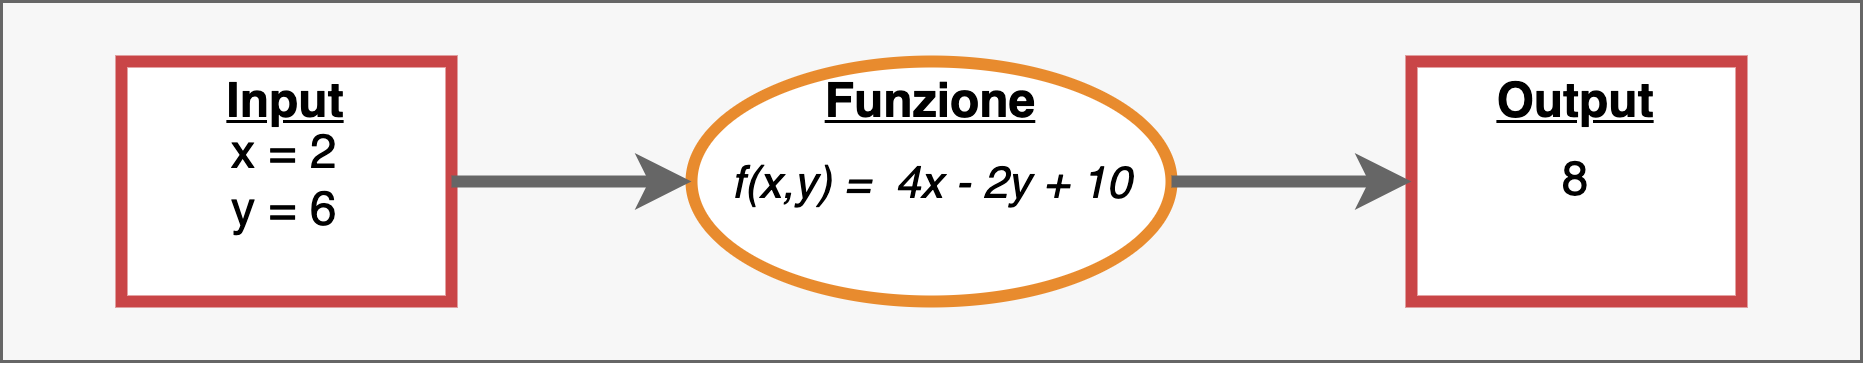
\includegraphics[width=0.95\textwidth,height=\textheight]{images/functions-graph.png}

Abbiamo già incontrato le nostre prime funzioni per eseguire specifiche operazioni matematiche nel Capitolo \ref{math-operators} come ad esempio \texttt{sqrt()} o \texttt{abs()} usate per ottenere ripettivamente la radice quadrata o il valore assoluto di un numero. Ovviamente le funzioni in R non sono limitate ai soli calcoli matematici ma possono eseguire qualsiasi genere di compito come ad esempio creare grafici e tabelle o manipolare dei dati o dei file. Tuttavia il concetto rimane lo stesso: ricevuti degli oggetti in input, le funzioni compiono determinate azioni e restituiscono dei nuovi oggetti in output.

In realtà incontreremo delle funzioni che non richiedono input o non produrre degli output. Ad esempio \texttt{getwd()} non richiede input oppure la funzione \texttt{rm()} non produce output. Tuttavia questo accade nella minoranza dei casi.

Per eseguire una funzione in R è necessario digitare il nome della funzione ed indicare tra parentesi i valori che vogliamo assegnare agli \textbf{argomenti} della funzione, ovvero i nostri input, separati da virgole. Generalmente si utilizza quindi la seguente sintassi:

\texttt{\textless{}nome-funzione\textgreater{}(\textless{}nome-arg1\textgreater{}\ =\ \textless{}valore-arg1\textgreater{},\ \textless{}nome-arg2\textgreater{}\ =\ \textless{}valore-arg2\textgreater{},...)}

{}

Ad esempio per creare una sequenza di valori con incrementi di 1 posso usare la funzione \texttt{seq()}, i cui argomenti sono \texttt{from} e \texttt{to} ed indicano rispettivamente il valore iniziale ed il valore massimo della sequenza.

\begin{Shaded}
\begin{Highlighting}[]
\CommentTok{# creo una sequenza di valori da 0 a 10 con incrementi di 1}
\KeywordTok{seq}\NormalTok{(}\DataTypeTok{from =} \DecValTok{0}\NormalTok{, }\DataTypeTok{to =} \DecValTok{10}\NormalTok{)}
\CommentTok{##  [1]  0  1  2  3  4  5  6  7  8  9 10}
\end{Highlighting}
\end{Shaded}

\hypertarget{argomenti-di-una-funzione}{%
\subsection{Argomenti di una Funzione}\label{argomenti-di-una-funzione}}

Nel definire gli argomenti di una funzione non è necessario specificare il nome degli argomenti. Ad esempio il comando precedente può essere eseguito anche specificando solamente i valori.

\begin{Shaded}
\begin{Highlighting}[]
\CommentTok{# creo una sequenza di valori da 0 a 10 con incrementi di 1}
\KeywordTok{seq}\NormalTok{(}\DecValTok{0}\NormalTok{, }\DecValTok{10}\NormalTok{)}
\CommentTok{##  [1]  0  1  2  3  4  5  6  7  8  9 10}
\end{Highlighting}
\end{Shaded}

Tuttavia, questo rende più difficile la lettura e la comprensione del codice poichè non è chiaro a quali argomenti si riferiscono i valori. L'ordine con cui vengono definiti i valori in questo caso è iportante, poichè R assume rispetti l'ordine prestabilito degli argomenti. Osserva come invertendo invertendo i valori ovviamente otteniamo risultati differenti da quelli precedenti, ma questo non avviene quando il nome dell'argomento è specificato.

\begin{Shaded}
\begin{Highlighting}[]
\CommentTok{# inverto i valori senza i nomi degli argomenti}
\KeywordTok{seq}\NormalTok{(}\DecValTok{10}\NormalTok{, }\DecValTok{0}\NormalTok{)}
\CommentTok{##  [1] 10  9  8  7  6  5  4  3  2  1  0}

\CommentTok{# inverto i valori con i nomi degli argomenti}
\KeywordTok{seq}\NormalTok{(}\DataTypeTok{to =} \DecValTok{10}\NormalTok{, }\DataTypeTok{from =} \DecValTok{0}\NormalTok{)}
\CommentTok{##  [1]  0  1  2  3  4  5  6  7  8  9 10}
\end{Highlighting}
\end{Shaded}

Vediamo inoltre come le funzioni possano avere molteplici argomenti, ma che non sia necessario specificare il valore per ognuno di essi. Molti argomenti, infatti, hanno già dei valori prestabiliti di \emph{default} e non richiedo quindi di essere specificati almeno che ovviamente non si vogliano utilizzare impostazioni diverse da quelle di \emph{default}. Oppure lo specificare un dato argomento rispetto ad un altro può definire il comportamento stesso della funzione.

Ad esempio la funzione \texttt{seq()} possiede anche gli argomenti \texttt{by} e \texttt{length.out} che prima non erano stati specificati. \texttt{by} permette di definire l'incremento per ogni elemento successivo della sequenza mentre \texttt{length.out} permette di definire il numero di elementi della sequenza. Vediamo come allo specificare dell'uno o dell'altro agromento (o di entrambi) il comportamento della funzione vari.

\begin{Shaded}
\begin{Highlighting}[]
\KeywordTok{seq}\NormalTok{(}\DataTypeTok{from =} \DecValTok{0}\NormalTok{,  }\DataTypeTok{to =} \DecValTok{10}\NormalTok{, }\DataTypeTok{by =} \DecValTok{5}\NormalTok{)}
\CommentTok{## [1]  0  5 10}
\KeywordTok{seq}\NormalTok{(}\DataTypeTok{from =} \DecValTok{0}\NormalTok{,  }\DataTypeTok{to =} \DecValTok{10}\NormalTok{, }\DataTypeTok{length.out =} \DecValTok{5}\NormalTok{)}
\CommentTok{## [1]  0.0  2.5  5.0  7.5 10.0}
\KeywordTok{seq}\NormalTok{(}\DataTypeTok{from =} \DecValTok{0}\NormalTok{,  }\DataTypeTok{to =} \DecValTok{10}\NormalTok{, }\DataTypeTok{length.out =} \DecValTok{5}\NormalTok{, }\DataTypeTok{by =} \DecValTok{4}\NormalTok{)}
\CommentTok{## Error in seq.default(from = 0, to = 10, length.out = 5, by = 4): too many arguments}
\end{Highlighting}
\end{Shaded}

E' pertanto cosigliabile esplicitare sempre gli argomenti di una funzione per rendere chiaro a che cosa si riferiscono i valori indicati. Questo è utlile anche per evitare eventuali comportamenti non voluti delle funzioni ad individuare più facilmente possibili errori.

Gli argomenti di una funzione, inoltre, richiedono specifiche tipologie e strutture di dati e sta a noi assicuraci che i dati siano forniti nel modo corretto. Vediamo ad esempio come la funzione \texttt{mean()} che calcola la media di un insieme di valori, richieda come input un vettore di valori numerici. Approfondiremo il concetto di vettori nel Capitolo TODO, al momento ci basta sapere che possiamo usare la funzione \texttt{c()} per combinare più valori in un unico vettore.

\begin{Shaded}
\begin{Highlighting}[]
\CommentTok{# Calcolo la media dei seguenti valori (numerici)}
\KeywordTok{mean}\NormalTok{(}\KeywordTok{c}\NormalTok{(}\DecValTok{10}\NormalTok{, }\DecValTok{6}\NormalTok{, }\DecValTok{8}\NormalTok{, }\DecValTok{12}\NormalTok{)) }\CommentTok{# c() combina più valori in un unico vettore}
\CommentTok{## [1] 9}

\KeywordTok{mean}\NormalTok{(}\DecValTok{10}\NormalTok{, }\DecValTok{6}\NormalTok{, }\DecValTok{8}\NormalTok{, }\DecValTok{12}\NormalTok{)}
\CommentTok{## [1] 10}
\end{Highlighting}
\end{Shaded}

Notiamo come nel primo caso il risultato sia corretto mentre nel secondo è sbagliato. Questo perchè \texttt{mean()} richiede come primo argomento il vettore su cui calcolare la media. Nel primo caso abbiamo correttamente specificato il vettore di valori usando la funzione \texttt{c()}. Nel secondo caso invece, il primo argomento risulta essere solo il valore \texttt{10} ed R calcola la media di \texttt{10} ovvero \texttt{10}. Gli altri valori sono passati ad altri argomenti che non alterano il comportameto ma neppure ci segnalano di questo importante errore.

Nel seguente esempio, possiamo vedere come \texttt{mean()} richieda che i valori siano numerici. Seppur \texttt{"1"} \texttt{"2"}, e \texttt{"3"} siano dei numeri, l'utilizzo delle doppie virgolette li rende delle stringhe di caratteri e non dei valori numerici e giustamente R non può eseguire una media su dei caratteri.

\begin{Shaded}
\begin{Highlighting}[]
\CommentTok{# Calcolo la media dei seguenti valori (caratteri)}
\KeywordTok{mean}\NormalTok{(}\KeywordTok{c}\NormalTok{(}\StringTok{"1"}\NormalTok{, }\StringTok{"2"}\NormalTok{, }\StringTok{"3"}\NormalTok{))}
\CommentTok{## Warning in mean.default(c("1", "2", "3")): argument is not numeric or logical:}
\CommentTok{## returning NA}
\CommentTok{## [1] NA}
\end{Highlighting}
\end{Shaded}

Capiamo quindi che per usare correttamente le funzioni è fondamentale conoscerne gli argomenti e rispettare le tipologie e strutture di dati richieste.

\hypertarget{help-i-need-somebodyhelp}{%
\subsection{Help! I need Somebody\ldots Help!}\label{help-i-need-somebodyhelp}}

Conoscere tutte le funzioni e tutti i loro argomenti è impossibile. Per fortuna R ci viene in soccorso fornendoci per ogni funzione la sua documentazione. Qui vengono fornite tutte le informazioni riguardanti la finalità della funzione, la descrizione dei suoi argomenti, i dettagli riguardanti i suoi possibili utilizzi.

Per accedere alla documentazione possiamo utilizzare il comando \texttt{?\textless{}nome-funzione\textgreater{}} oppure \texttt{help(\textless{}nome-funzione\textgreater{})}. Ad esempio:

\begin{Shaded}
\begin{Highlighting}[]
\NormalTok{?seq}
\KeywordTok{help}\NormalTok{(seq)}
\end{Highlighting}
\end{Shaded}

Una pagina si aprirà nel pannello ``Help'' in basso a destra con la documentazione della funzione in modo simile a quanto rappresentato in Figura \ref{fig:help-page}.

\begin{figure}

{\centering 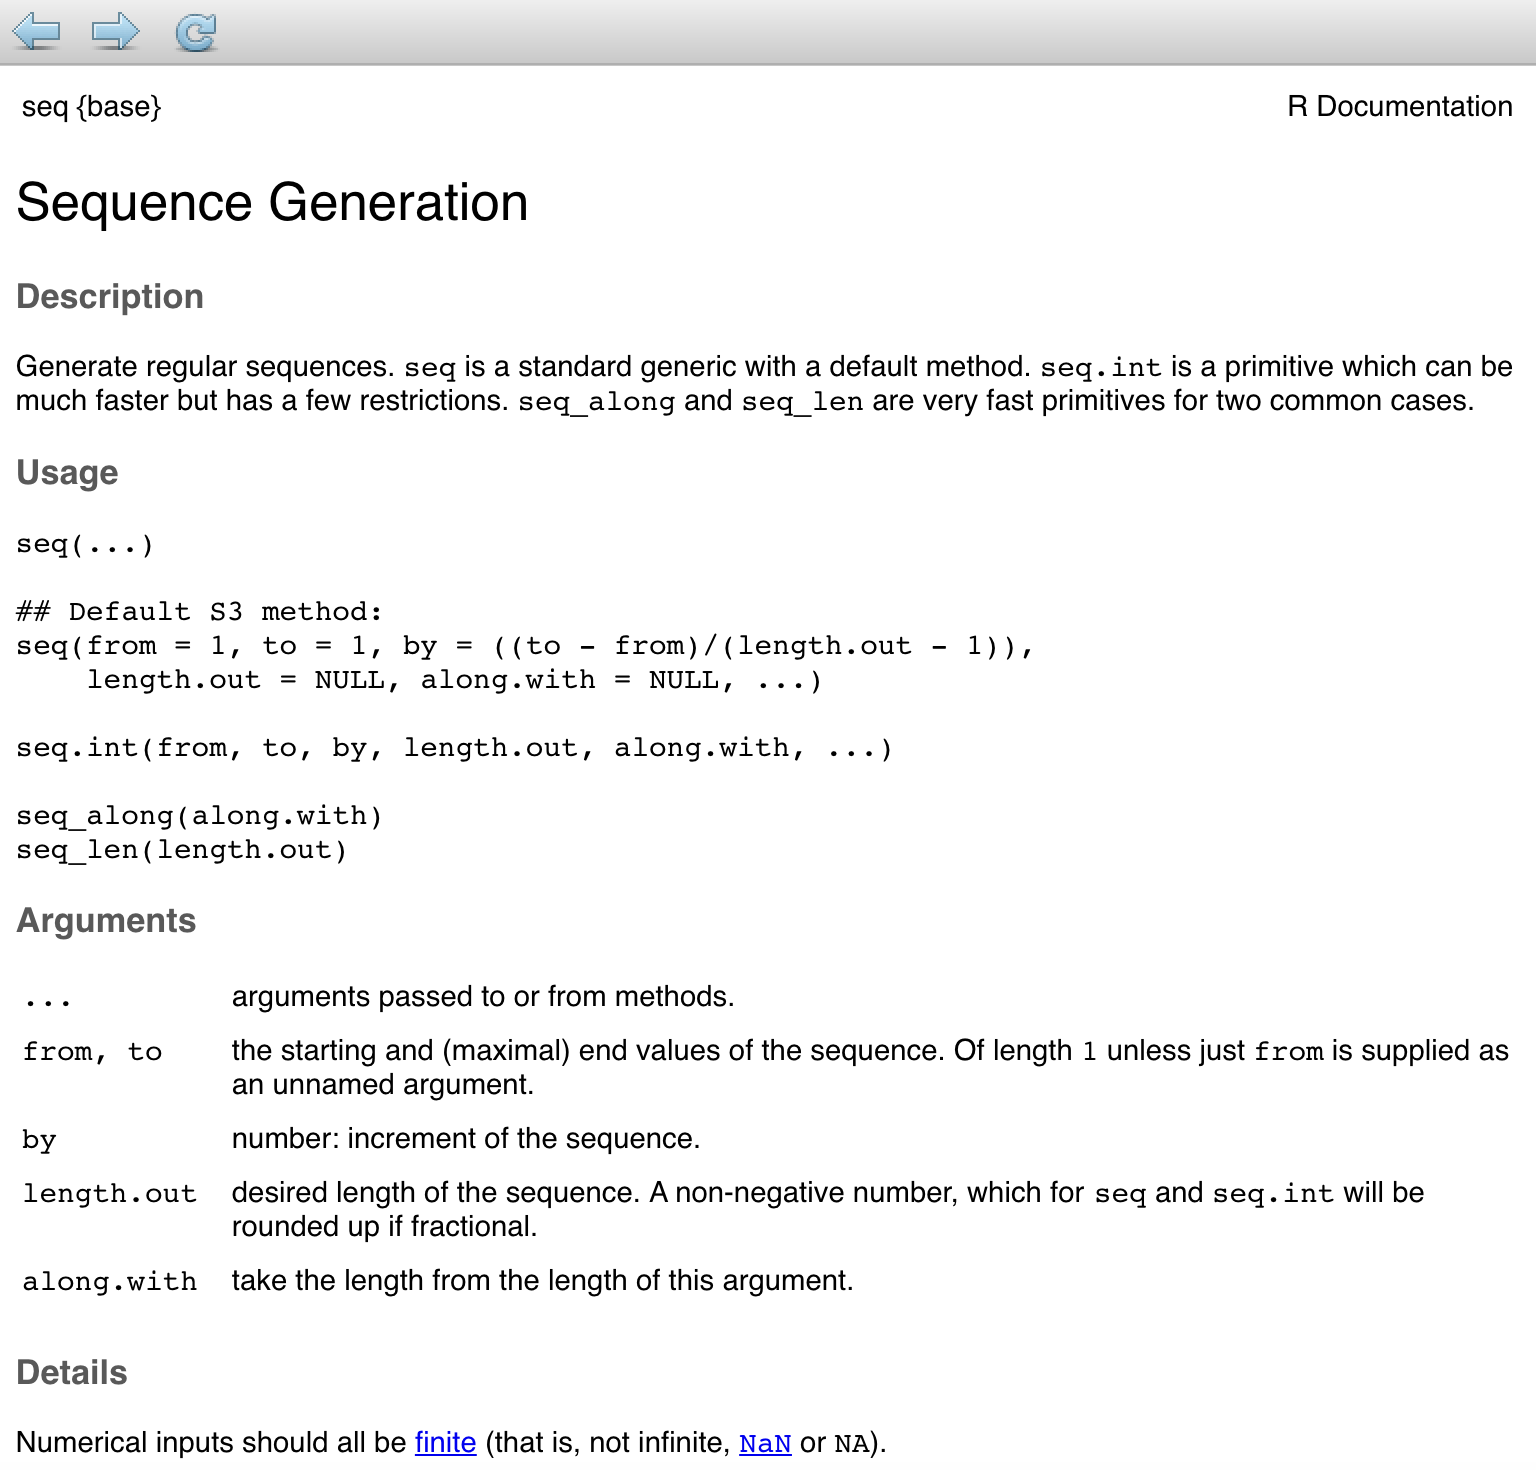
\includegraphics[width=0.85\linewidth]{images/help-seq} 

}

\caption{Help-page della funzione seq()}\label{fig:help-page}
\end{figure}

Il formato e le informazioni presenti nella pagina seguono delle norme comuni ma non obbligatorie. Infatti, non necessariamente vengono usati sempre tutti i campi e comunque all'autore delle funzioni è lasciato un certo grado di libertà nel personalizzare la documentazione. Tra i campi principali e più comunemente usati abbiamo:

\begin{itemize}
\tightlist
\item
  \textbf{Tiolo} - Titolo esplicativo della finalità della funzione\\
\item
  \textbf{Description} - Descrizione coincisa della funzione
\item
  \textbf{Usage} - Viene mostrata la struttura della funzione con i suoi argomenti e valori di default
\item
  \textbf{Arguments} - Elenco con la descrizione dettagliata di tutti gli argomenti. Qui troviamo per ogni argomento sia le opzioni utilizzabili ed il loro effetto, che la tipologia di valori richiesti
\item
  \textbf{Details} - Descrizione dettagliata della funzione considerando i casi di utilizzo ed eventuali note tecniche
\item
  \textbf{Value} - Descrizione dell'output dalla funzione. Qui troviamo sia la descrizione della struttura dei dati dell'output che la descrizione dei suei elementi utile per interpretare ed utilizzare i rsultati ottenuti
\item
  \textbf{See Also} - Eventuali link ad altre funzioni simili o in relazione con la nostra funzione
\item
  \textbf{Examples} - Esempi di uso della funzione
\end{itemize}

\begin{trick}[Autocompletamento with 'Tab']

La natura dei programmatori è essere pigri e smemorati. Per fortuna ogni \emph{code editor} che si rispetti (i.e., programma per la scrittura di codici) possiede delle utli funzioni di autocompletamento e suggerimento dei comandi che semplificano la scrittura di codici.

In Rstudio, i suggerimenti compaino automaticamente durante la scrittura di un comando oppure possono essere richiamati premendo il tasto \texttt{Tab} in alto a sinistra della tastiera ( 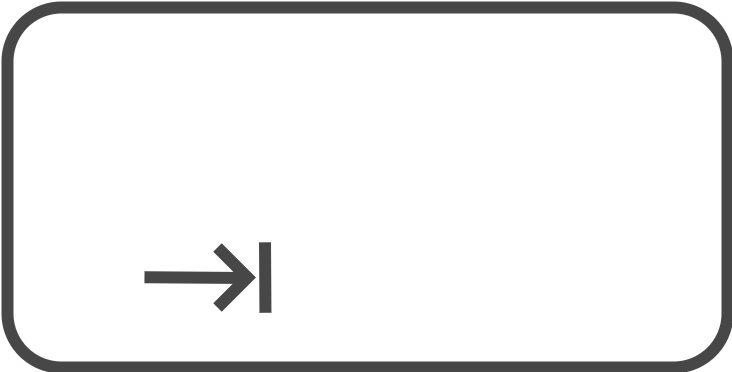
\includegraphics[width=0.05\textwidth,height=\textheight]{images/Tab.png} ). Comparirà una finestra con possibili soluzioni di autocompletamento del nome della funzione. Utilizzando le frecce della tastiera possiamo evidenziare lq funzione voluta e premere \texttt{Invio} per autocompletare il comando. Nota come accanto al nome della funzione appare anche un piccolo riquadro giallo con la descrizione della funzione.

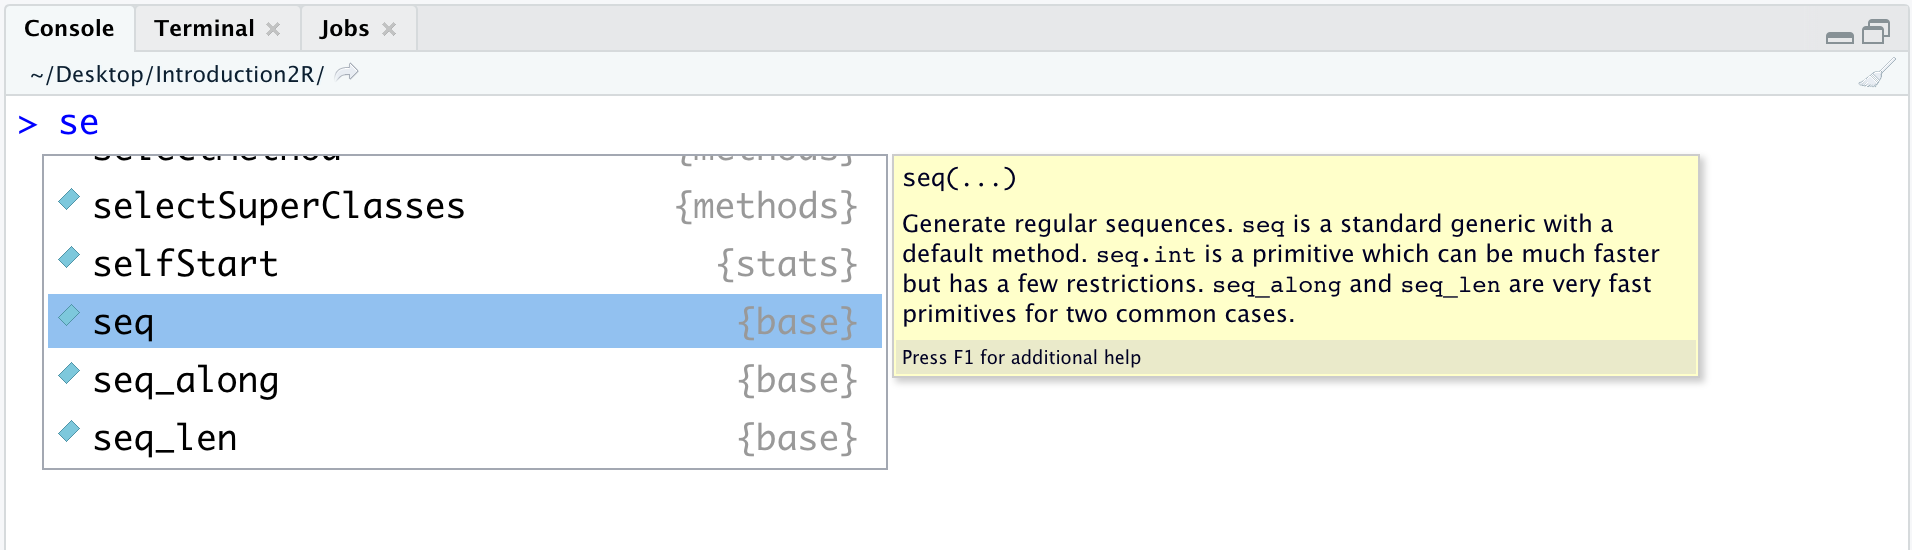
\includegraphics[width=0.95\textwidth,height=\textheight]{images/autocomplete-function.png}

Per inserire gli argomenti della funzione possiamo fare affidamento nuovamente ai suggerimenti e alla funzione di autocompletamento. Sarà sufficiente premere nuovamente il tasto \texttt{Tab} e questa volta comparirà una lista degli argomenti con la relativa descrizione. Sarà quindi sufficiente selezionare con le frecce l'argomento desiderato e premere \texttt{Invio}.

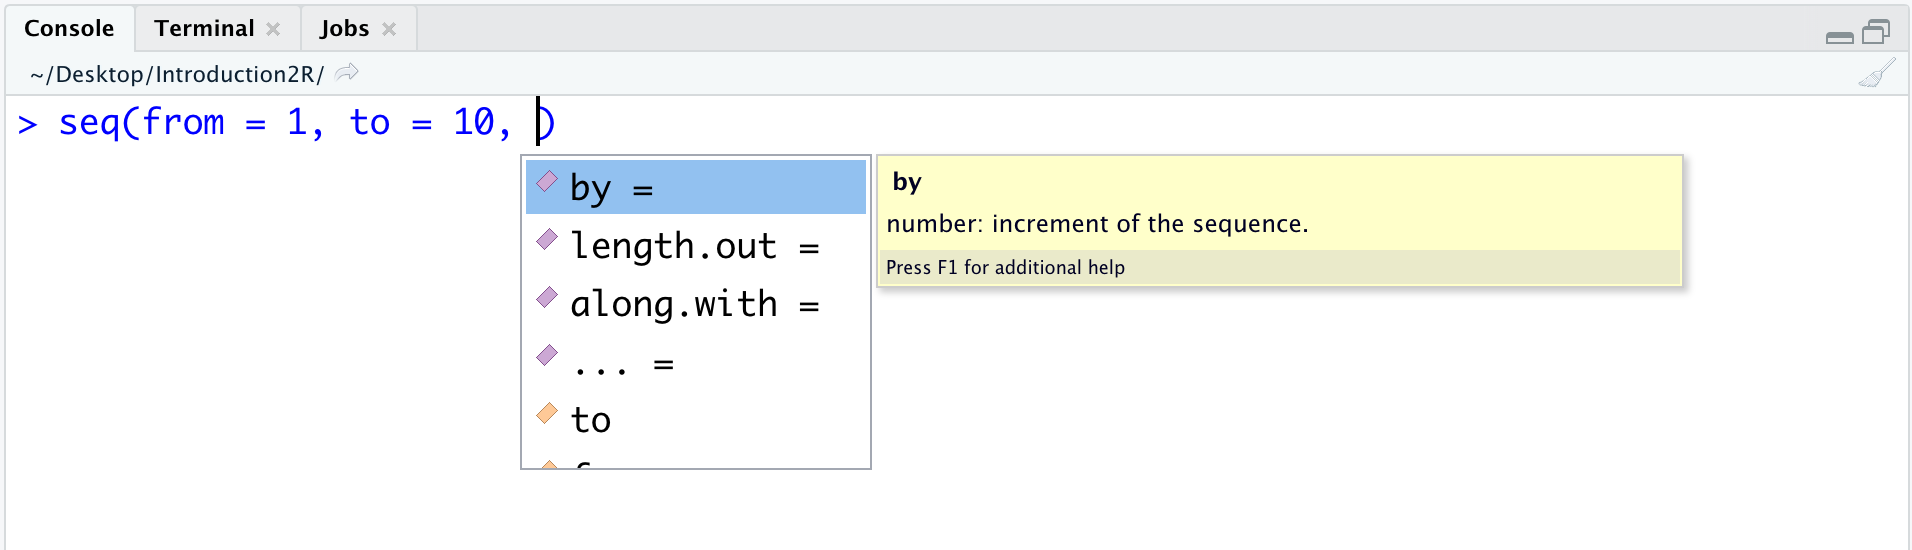
\includegraphics[width=0.95\textwidth,height=\textheight]{images/autocomplete-arguments.png}

Notate come la funzione di autocompletamento non sia utilizzata solo per le funzioni ma anche per i nomi degli oggetti. Questo ci consentirà di richiamare velocemente oggetti precedentemente creati evitando di digitare l'intero nome.

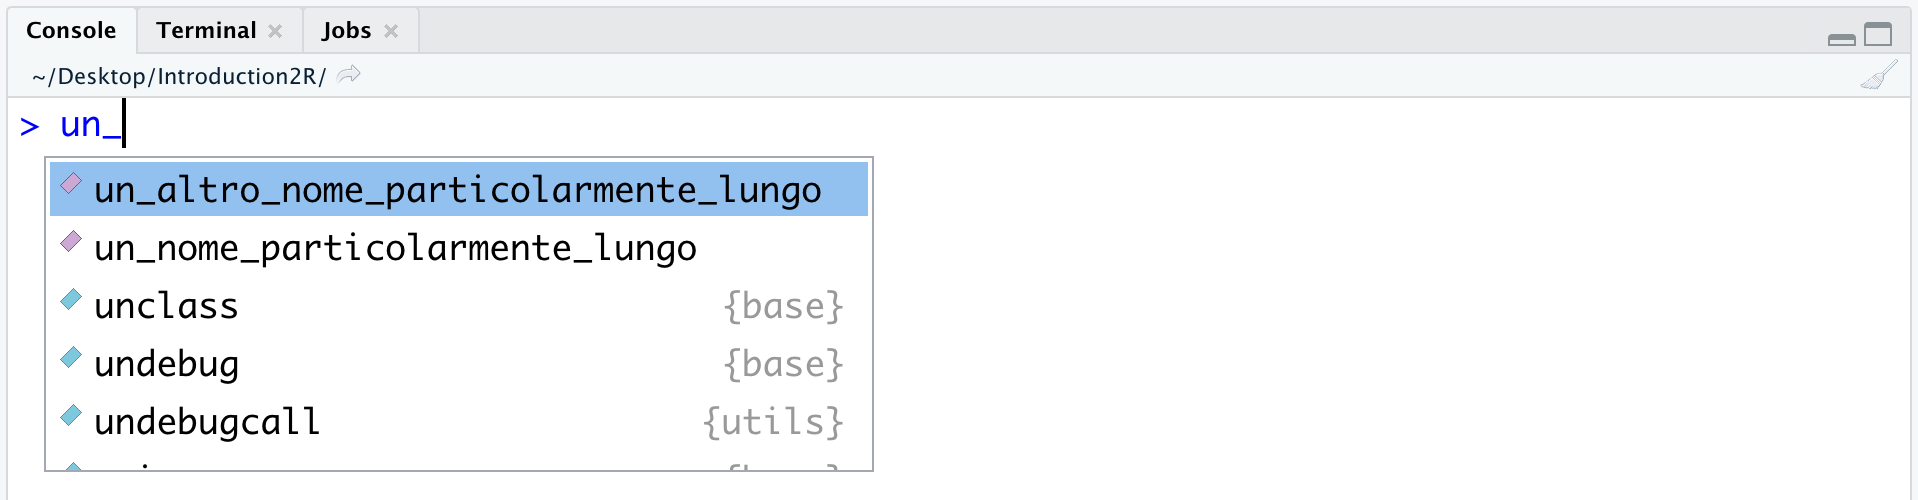
\includegraphics[width=0.95\textwidth,height=\textheight]{images/autocomplete-objects.png}

\end{trick}

\hypertarget{working-session}{%
\chapter{Sessione di Lavoro}\label{working-session}}

In queso capitolo introdurremo alcuni concetti molto importanti che riguardano le sessioni di lavoro in R o RStudio. In particolare parleremo dell'\emph{environment}, della \emph{working directory} e dell'utilizzo di pacchetti.

Infine, disuteremo di alcuni aspetti generali della programmazione quali la gestione dei messaggi di errore o \emph{warnings} e vedremo alcune buone norme riguardanti l'organizzazione degli scripts e l'uso degli \emph{RStudio Projects} per essere ordinati ed efficaci nelle proprie sessioni di lavoro.

\hypertarget{environment}{%
\section{Environment}\label{environment}}

Nel Capitolo \ref{objects-section}, abbiamo visto come sia possibile assegnare dei valori a degli oggetti. Questi oggetti vengono creati nel nostro ambiente di lavoro (o meglio \emph{Environment}) e potranno essere utilizzati in seguito.

Il nostro Enviroment raccoglie quindi tutti gli oggetti che vengono creati durante la nostra sessione di lavoro. E' possibile valutare gli oggetti attualmente presenti osservando il pannello \emph{Envrionmen} in alto a destra (vedi Figura \ref{fig:environment2}) oppure utilizzadno il comando \texttt{ls()}, ovvero \emph{list objects}.

\begin{figure}

{\centering 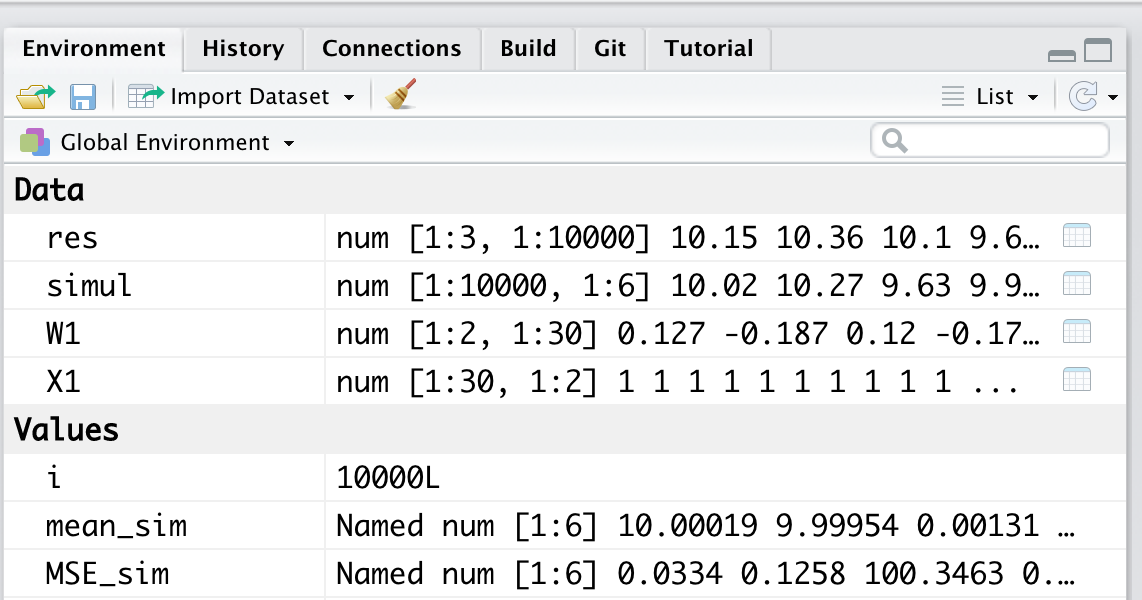
\includegraphics[width=0.6\linewidth]{images/environment} 

}

\caption{*Environment* - Elenco degli oggetti e variabili presenti nel'ambiente di lavoro}\label{fig:environment2}
\end{figure}

All'inizio della sessione di lavoro il nostro Environment sarà vuoto ().

\begin{figure}

{\centering 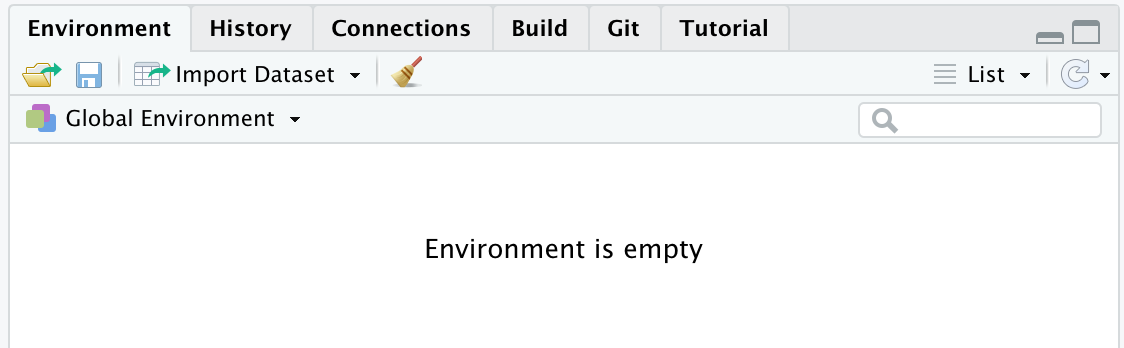
\includegraphics[width=0.6\linewidth]{images/environment-empty} 

}

\caption{*Environment* vuoto ad inizio sessione di lavoro}\label{fig:environment-empty}
\end{figure}

\begin{Shaded}
\begin{Highlighting}[]
\CommentTok{# Environment vuoto}
\KeywordTok{ls}\NormalTok{()}
\CommentTok{## character(0)}
\end{Highlighting}
\end{Shaded}

\begin{Shaded}
\begin{Highlighting}[]
\CommentTok{# Creo oggetti}
\NormalTok{x <-}\StringTok{  }\KeywordTok{c}\NormalTok{(}\DecValTok{2}\NormalTok{,}\DecValTok{4}\NormalTok{,}\DecValTok{6}\NormalTok{,}\DecValTok{8}\NormalTok{)}
\NormalTok{y <-}\StringTok{  }\DecValTok{27}
\NormalTok{word <-}\StringTok{ "Hello Word!"}

\CommentTok{# Lista nomi oggetti nell'Environment}
\KeywordTok{ls}\NormalTok{()}
\CommentTok{## [1] "word" "x"    "y"}
\end{Highlighting}
\end{Shaded}

\begin{figure}

{\centering 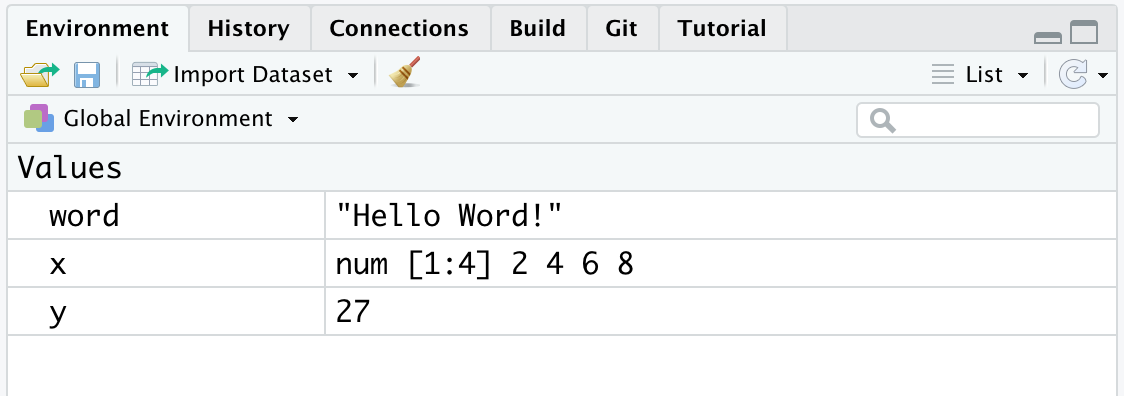
\includegraphics[width=0.6\linewidth]{images/environment-objects} 

}

\caption{*Environment* contenente gli oggetti creati}\label{fig:environment-object}
\end{figure}

\begin{itemize}
\item
  concetto di ambiente di lavoro
\item
  ls()
\item
  rm()
\item
  tip box aspetto transirorio (vedremo successivamente come salvare caricare dati)
\end{itemize}

\hypertarget{working-directory}{%
\section{Working Directory}\label{working-directory}}

\begin{itemize}
\item
  che cosa è un path
\item
  home directory \textasciitilde{} (non mi ricordo se per windows lavora)
\item
  getwd();
\item
  setwd(); altri modi per settare al working directory
\item
  abodolute/relative path (?)
\end{itemize}

\hypertarget{r-packages}{%
\section{R-packages}\label{r-packages}}

\begin{itemize}
\item
  scaricare
\item
  library
\item
  uso funzioni
\item
  aggiornare i pacchetti
\item
  box tip per l'uso di ::
\end{itemize}

\hypertarget{errors-and-warnings}{%
\section{Errors and warnings}\label{errors-and-warnings}}

\hypertarget{sessione-di-lavoro}{%
\section{Sessione di lavoro}\label{sessione-di-lavoro}}

\begin{itemize}
\tightlist
\item
  pulizia script
\item
  commenti
\item
  sezioni script
\item
  settings
\item
  sintassi (gli spazi e gli indent corretti alineamenti)
\item
  idea di organizzare in vairi script, cartelle
\end{itemize}

\hypertarget{r-projects}{%
\subsection{R projects}\label{r-projects}}

\hypertarget{problema-google-soluzione}{%
\section{Problema + Google = Soluzione}\label{problema-google-soluzione}}

Quando si approccia la scrittura di codice, anche molto semplice la cosa che sicuramente capiterà più spesso sarà riscontrare \textbf{errori} e quindi trovare il modo per risolverli.

\begin{quote}
Qualche programmatore esperto direbbe che l'essenza stessa di programmare è in realtà risolvere gli errori che il codice produce.
\end{quote}

L'\textbf{errore non è quindi un difetto o un imprevisto}, ma parte integrante della scrittura del codice. L'importante è capire come gestirlo.

Abbiamo tutti le immagini in testa di programmatori da film che scrivono codice alla velocità della luce, quando nella realtà dobbiamo spesso affrontare \textbf{bug}, \textbf{errori di output} o altri problemi vari. Una serie di skills utili da imparare sono:

\begin{itemize}
\tightlist
\item
  Comprendere a fondo gli \textbf{errori} (non banale)
\item
  Sapere \textbf{come e dove cercare una soluzione} (ancora meno banale)
\item
  In caso non si trovi una soluzione direttamente, chiedere aiuto in modo efficace
\end{itemize}

\hypertarget{comprendere-gli-errori}{%
\subsubsection*{Comprendere gli errori}\label{comprendere-gli-errori}}
\addcontentsline{toc}{subsubsection}{Comprendere gli errori}

Rispetto agli errori, R è solitamente abbastanza esplicito nel farci capire il problema. Ad esempio usare una funzione di un pacchetto che non è stato caricato di solito fornisce un messaggio del tipo \texttt{Error\ in\ funzione\ :\ could\ not\ find\ function\ "funzione"}.

\hypertarget{ricercare-soluzioni}{%
\subsubsection*{Ricercare soluzioni}\label{ricercare-soluzioni}}
\addcontentsline{toc}{subsubsection}{Ricercare soluzioni}

Altre situazioni o messaggi potrebbero non essere altrettanto immediati, in quel caso Google è il nostro miglior amico.

Cercando infatti il messaggio di errore/warning su Google, al 99\% avremo altre persone che hanno avuto lo stesso problema e probabilmente anche una soluzione.

\begin{trick}[Ricerca su Google]

Il modo migliore per cercare è copiare e incollare su Google direttamente l'output di errore di R come ad esempio \texttt{Error\ in\ funzione\ :\ could\ not\ find\ function\ "funzione"} piuttosto che descrivere a parole il problema. I messaggi di errore sono standard per tutti, la tua descrizione invece no.

\end{trick}

Cercando in questo modo vedrete che molti dei risultati saranno esattamente riferiti al vostro errore:

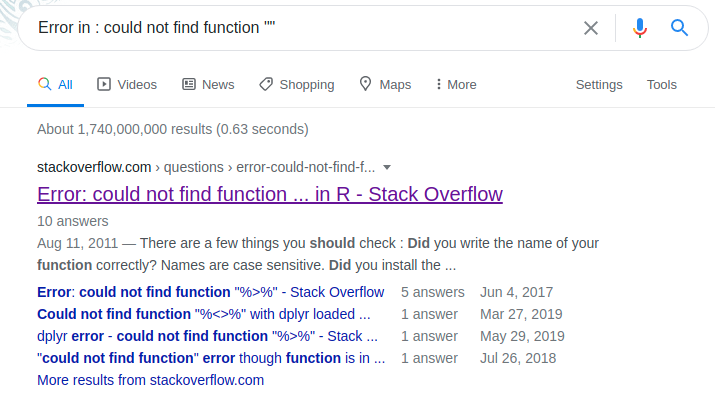
\includegraphics{images/stack_question.png}

\hypertarget{chiedere-una-soluzione}{%
\subsubsection{Chiedere una soluzione}\label{chiedere-una-soluzione}}

Se invece il vostro probelma non è un messaggio di errore ma un utilizzo specifico di R allora il consiglio è di usare una ricerca del tipo: \texttt{argomento\ +\ breve\ descrizione\ problema\ +\ R}. Nelle sezioni successive vedrete nel dettaglio altri aspetti della programmazione ma se volete ad esempio calcolare la \textbf{media} in R potrete scrivere \texttt{compute\ mean\ in\ R}.
Mi raccomando, fate tutte le ricerche in \textbf{inglese} perchè le possibilità di trovare una soluzione sono molto più alte.

Dopo qualche ricerca, vi renderete conto che il sito che vedrete più spesso si chiama \href{https://stackoverflow.com/}{\textbf{Stack Overflow}}. Questo è una manna dal cielo per tutti i programmatori, a qualsiasi livello di expertise. E' una community dove tramite domande e risposte, si impara a risolvere i vari problemi ed anche a trovare nuovi modi di fare la stessa cosa. E' veramente utile oltre che un ottimo modo per imparare.

L'ultimo punto di questa piccola guida alla ricerca di soluzioni, riguarda il fatto di dover non solo cercare ma anche chiedere. Dopo aver cercato vari post di persone che richiedevano aiuto per un problema noterete che le domande e le risposte hanno sempre una struttura simile. Questo non è solo un fatto stilistico ma anzi è molto utile per uniformare e rendere chiara la domanda ma sopratutto la risposta, in uno spirito di condivisione. C'è anche una \href{https://stackoverflow.com/help/how-to-ask}{guida dedicata} per scrivere la domanda perfetta.

In generale\footnote{Fonte: \href{https://codeblog.jonskeet.uk/2010/08/29/writing-the-perfect-question/}{Writing the perfect question - Jon Skeet}}:

\begin{itemize}
\tightlist
\item
  Titolo: un super riassunto del problema
\item
  Contesto: linguaggio (es. R), quale sistema operativo (es. Windows)
\item
  Descrizione del problema/richiesta: in modo chiaro e semplice ma non troppo generico
\item
  Codice ed eventuali dati per capire il problema
\end{itemize}

L'ultimo punto di questa lista è forse il più importante e si chiama in gergo tecnico \href{https://community.rstudio.com/t/faq-whats-a-reproducible-example-reprex-and-how-do-i-create-one/5219}{\textbf{REPREX}} (\textbf{Rep}roducible \textbf{Ex}ample). E' un tema leggermente più avanzato ma l'idea di fondo è quella di fornire tutte le informazioni possibili per poter riprodurre (e quindi eventualmente trovare una soluzione) il codice di qualcuno nel proprio computer.

Se vi dico ``R non mi fa creare un nuovo oggetto, quale è l'errore?'' è diverso da dire ``il comando \texttt{oggetto\ -\textgreater{}\ 10} mi da questo errore \texttt{Error\ in\ 10\ \textless{}-\ oggetto\ :\ invalid\ (do\_set)\ left-hand\ side\ to\ assignment}, come posso risolvere?''

\begin{tip}[My title]

Ci sono anche diversi pacchetti in R che rendono automatico creare questi esempi di codice da poter condividere, come il pacchetto \href{https://www.tidyverse.org/help/}{\texttt{reprex}}.

\end{tip}

\hypertarget{part-struttura-dati}{%
\part*{Struttura Dati}\label{part-struttura-dati}}
\addcontentsline{toc}{part}{Struttura Dati}

\hypertarget{introduzione}{%
\chapter*{Introduzione}\label{introduzione}}
\addcontentsline{toc}{chapter}{Introduzione}

Working in progress.

\hypertarget{data-type}{%
\chapter{Data Type}\label{data-type}}

Working in progress.

Tipi di vettori

In R ci sono 4 tipi differenti di vettori: numerici, logici, caratteri e fattori.

\hypertarget{vettori-numerici}{%
\section{Vettori Numerici}\label{vettori-numerici}}

I vettori numerici sono utilizzati per compiere operazioni aritmetiche, in R sono indicati come \texttt{num}. In R ci sono è possibil e specificare se i numeri contenuti nel vettore sono numeri interi, avremmo quindi un vettore di valori interi (indicato in R come \texttt{int}). Per fare ciò è possibile aggiungere \texttt{L} ad ogni valore numerico nel definire il vettore oppure usare la funzione \texttt{as.integer()} per trasformare un vettore numerico in un vettore intero.

\textbf{Esempio:}

\begin{Shaded}
\begin{Highlighting}[]
\NormalTok{x <-}\StringTok{ }\KeywordTok{c}\NormalTok{(4L, 6L, 12L, 34L, 8L)}

\NormalTok{x <-}\StringTok{ }\KeywordTok{as.integer}\NormalTok{(}\KeywordTok{c}\NormalTok{(}\DecValTok{4}\NormalTok{, }\DecValTok{6}\NormalTok{, }\DecValTok{12}\NormalTok{, }\DecValTok{34}\NormalTok{, }\DecValTok{8}\NormalTok{))}
\end{Highlighting}
\end{Shaded}

\textbf{Nota}: per trasformare un vettore intero in un vettore numerico è possibile usare la funzione \texttt{as.numeric()}.

\hypertarget{vettori-logici}{%
\section{Vettori logici}\label{vettori-logici}}

I vettori logici sono formati dai volori \texttt{TRUE} e \texttt{FALSE}, che possono essere abbreviati rispettivamente in \texttt{T} e \texttt{F}. In R i vettori logici sono indicati come \texttt{logi}. In genere, i vettori logici sono il risultato delle operazioni in cui viene chiesto ad R di valutare la condizione logica di una proposizione.

\begin{Shaded}
\begin{Highlighting}[]
\NormalTok{x}\OperatorTok{>}\DecValTok{10}
\end{Highlighting}
\end{Shaded}

\begin{verbatim}
## [1] FALSE FALSE  TRUE  TRUE FALSE
\end{verbatim}

\textbf{Nota:} in R, come in molti altri software di programmazione, \texttt{TRUE} assume il valore numerico \texttt{1} e \texttt{FALSE} assume il valore \texttt{0}.

\begin{Shaded}
\begin{Highlighting}[]
\KeywordTok{sum}\NormalTok{(x}\OperatorTok{>}\DecValTok{10}\NormalTok{)}
\end{Highlighting}
\end{Shaded}

\begin{verbatim}
## [1] 2
\end{verbatim}

E' possibile trasformare un vettore numerico in un vettor logico attraverso la funzione \texttt{as.logical()}, gli \texttt{0} assumeranno il valore \texttt{FALSE} mentre qualsiasi altro numero assumerà il valore \texttt{TRUE}.

\begin{Shaded}
\begin{Highlighting}[]
\KeywordTok{as.logical}\NormalTok{(}\KeywordTok{c}\NormalTok{(}\DecValTok{1}\NormalTok{,}\DecValTok{0}\NormalTok{,.}\DecValTok{034}\NormalTok{,}\OperatorTok{-}\DecValTok{1}\NormalTok{,}\DecValTok{0}\NormalTok{,}\DecValTok{8}\NormalTok{))}
\end{Highlighting}
\end{Shaded}

\begin{verbatim}
## [1]  TRUE FALSE  TRUE  TRUE FALSE  TRUE
\end{verbatim}

\hypertarget{vettori-di-caratteri}{%
\section{Vettori di caratteri}\label{vettori-di-caratteri}}

I vettori di caratteri contengono stringhe di caratteri e sono indicati in R con `chr\}. Non è possibile eseguire operazioni aritmetiche con vettori di caratteri ma solo valutare se due stringhe sono uguali o differenti.

\begin{Shaded}
\begin{Highlighting}[]
\NormalTok{j<-}\KeywordTok{c}\NormalTok{(}\StringTok{"Hello"}\NormalTok{,}\StringTok{"World"}\NormalTok{,}\StringTok{"hello"}\NormalTok{,}\StringTok{"world"}\NormalTok{)}
\NormalTok{j}\OperatorTok{==}\StringTok{"hello"}
\end{Highlighting}
\end{Shaded}

\begin{verbatim}
## [1] FALSE FALSE  TRUE FALSE
\end{verbatim}

Per trasformare un vettore qualsiasi in una vettore di caratteri e possibile usare la funzione \texttt{as.character()}.

\begin{Shaded}
\begin{Highlighting}[]
\KeywordTok{as.character}\NormalTok{(x)}
\end{Highlighting}
\end{Shaded}

\begin{verbatim}
## [1] "4"  "6"  "12" "34" "8"
\end{verbatim}

\begin{Shaded}
\begin{Highlighting}[]
\KeywordTok{as.character}\NormalTok{(x}\OperatorTok{>}\DecValTok{10}\NormalTok{)}
\end{Highlighting}
\end{Shaded}

\begin{verbatim}
## [1] "FALSE" "FALSE" "TRUE"  "TRUE"  "FALSE"
\end{verbatim}

\hypertarget{vector}{%
\chapter{Vettori}\label{vector}}

Working in progress

\hypertarget{creazione-di-vettori}{%
\section{Creazione di Vettori}\label{creazione-di-vettori}}

In R per definire un vettore si utilizza il comando \texttt{\textless{}nome-vettore\textgreater{}\ \textless{}-\ c(\textless{}oggetti\textgreater{})}. Ricorda che gli elementi devono essere separati da una virgola.

\hypertarget{esercizi-2}{%
\subsection*{Esercizi}\label{esercizi-2}}
\addcontentsline{toc}{subsection}{Esercizi}

\begin{enumerate}
\def\labelenumi{\arabic{enumi}.}
\tightlist
\item
  Crea il vettore \texttt{x} contenente i numeri 4, 6, 12, 34, 8
\item
  Crea il vettore \texttt{y} contenente tutti i numeri pari compresi tra 1 e 25 (\texttt{?seq()})
\item
  Crea il vettore \texttt{z} contenente tutti i primi 10 multipli di 7 partendo da 13 (\texttt{?seq()})
\item
  Crea il vettore \texttt{s} in cui le lettere \texttt{"A"},\texttt{"B"} e \texttt{"C"} vengono ripetute nel medesimo ordine 4 volte (\texttt{?rep()}).
\item
  Crea il vettore \texttt{t} in cui le letter \texttt{"A"},\texttt{"B"} e \texttt{"C"} vengono ripetute ognuna 4 volte (\texttt{?rep()}).
\end{enumerate}

\hypertarget{selezione-elementi-di-un-vettore}{%
\section{Selezione Elementi di un Vettore}\label{selezione-elementi-di-un-vettore}}

In R per selezioneare gli elementi di un vettore si deve indicare all'interno delle parentesi quadre la \textbf{posizione degli elementi} da selezionare, non il valore dell'elemento stesso:

\texttt{\textless{}nome-vettore\textgreater{}{[}\textless{}indice-posizione\textgreater{}{]}}\textbackslash{}
In alternativa si puù definire la condizione logica che gli elementi che si vogliono selezionare devono rispettare.

Per *\textbackslash textbf\{\textbf{eliminare degli elementi} da un vettore si utilizza all'interno delle parentesi quadre l'operatore ``-'' insieme agli indici di posizione degli elementi da eliminare (esempio: \texttt{x{[}c(-2,-4){]}} oppure \texttt{x{[}-c(2,4){]}}).

\hypertarget{esercizi-3}{%
\subsection*{Esercizi}\label{esercizi-3}}
\addcontentsline{toc}{subsection}{Esercizi}

\begin{enumerate}
\def\labelenumi{\arabic{enumi}.}
\tightlist
\item
  Del vettore \texttt{x} seleziona il 2°, 3° e 5° elemento
\item
  Del vettore \texttt{y} seleziona tutti i valori minori di 13 o maggiori di 19
\item
  Del vettore \texttt{z} seleziona tutti i valori compresi tra 24 e 50
\item
  Elimina dal vettore \texttt{z} i valori 28 e 42
\item
  Del vettore \texttt{s} seleziona tutti gli elementi uguali ad ``A''
\item
  Del vettore \texttt{t} seleziona tutti gli elementi diversi da ``B''.
\end{enumerate}

\hypertarget{funzioni-ed-operazioni-tra-vettori}{%
\section{Funzioni ed Operazioni tra Vettori}\label{funzioni-ed-operazioni-tra-vettori}}

Per compiere operazioni tra vettori è necessario che essi abbiano identica lunghezza.

\begin{table}[!h]

\caption{\label{tab:table-vector-operators}Operazioni con vettori}
\centering
\begin{tabular}[t]{l|l}
\hline
Operazione & Nome\\
\hline
\texttt{<nuovo-vettore> <- c(<vettore1>, <vettore2>)} & Per unire più vettori in un unico vettore\\
\hline
\texttt{length(<nome-vettore>)} & Per valutare il numero di elementi contenuti in un vettore\\
\hline
\texttt{vettore1 + vettore2} & Somma di due vettori\\
\hline
\texttt{vettore1 - vettore2} & Differenza tra due vettori\\
\hline
\texttt{vettore1 * vettore2} & Prodotto tra due vettori\\
\hline
\texttt{vettore1 / vettore2} & Rapporto tra due vettori\\
\hline
\end{tabular}
\end{table}

\textbf{Nota:} In R il prodotto e rapporto tra vettori sono eseguiti elemento per elemento (al contrario di molti altri software).

\hypertarget{esercizi-4}{%
\subsection*{Esercizi}\label{esercizi-4}}
\addcontentsline{toc}{subsection}{Esercizi}

\begin{enumerate}
\def\labelenumi{\arabic{enumi}.}
\tightlist
\item
  Crea il vettore \texttt{j} unendo i vettori \texttt{x} ed \texttt{z}.
\item
  Elimina gli ultimi tre elementi del vettore \texttt{j} e controlla che i vettori \texttt{j} e \texttt{y} abbiano la stessa lunghezza.
\item
  Calcola la somma tra i vettori \texttt{j} e \texttt{y}.
\item
  Moltiplica il vettore z per una costante \texttt{k=3}.
\item
  Calcola il prodotto tra i primi 10 elementi del vettore \texttt{y} ed il vettore \texttt{z}.
\end{enumerate}

\hypertarget{factors}{%
\chapter{Fattori}\label{factors}}

Working in progress.

I fattori sono utilizzati per definire delle variabili categoriali, sono indicati in R con \texttt{Factor}. Per creare una variabile categoriale in R si utilizza la funzione:

\texttt{nome\_variabile\textless{}-factor(c(...,\ data,\ ...),\ levels=c(...))}

L'opzione \texttt{levels=c(...)} è usata per specificare quali sono i possibili livelli della variabile categoriale. E' possibile modificare o aggiungere nuovi livelli della variabile anche in un secondo momento utilizzando la funzione:

\texttt{levels(nome\_fattore)\textless{}-\ c(...,\ nuovi\_livelli,\ ...)}

\textbf{Nota}: nel creare un fattore R associa ad ogni livello un valore in ordine crescente e assegna agli elementi del vettore il loro volore numerico a seconda del proprio livello. Pertanto se un fattore è trasformato in un vettore numerico vengono restituiti tali valori numerici e non i livelli anche nel caso fossero dei numeri. Prendiamo per esempio la variabile \texttt{anni\_istruzione}:

\begin{Shaded}
\begin{Highlighting}[]
\NormalTok{anni_istruzione<-}\KeywordTok{factor}\NormalTok{(}\KeywordTok{c}\NormalTok{(}\DecValTok{11}\NormalTok{,}\DecValTok{8}\NormalTok{,}\DecValTok{4}\NormalTok{,}\DecValTok{8}\NormalTok{,}\DecValTok{11}\NormalTok{,}\DecValTok{4}\NormalTok{,}\DecValTok{11}\NormalTok{,}\DecValTok{8}\NormalTok{))}
\NormalTok{anni_istruzione}
\CommentTok{## [1] 11 8  4  8  11 4  11 8 }
\CommentTok{## Levels: 4 8 11}
\KeywordTok{as.numeric}\NormalTok{(anni_istruzione)}
\CommentTok{## [1] 3 2 1 2 3 1 3 2}
\end{Highlighting}
\end{Shaded}

Per riottenere gli estti valori numerici è necessario eseguire:

\begin{Shaded}
\begin{Highlighting}[]
\KeywordTok{as.numeric}\NormalTok{(}\KeywordTok{as.character}\NormalTok{(anni_istruzione))}
\CommentTok{## [1] 11  8  4  8 11  4 11  8}
\end{Highlighting}
\end{Shaded}

\hypertarget{esercizi-5}{%
\subsection*{Esercizi}\label{esercizi-5}}
\addcontentsline{toc}{subsection}{Esercizi}

\begin{enumerate}
\def\labelenumi{\arabic{enumi}.}
\tightlist
\item
  Crea la variabile categoriale \texttt{sex} così definita:
\end{enumerate}

\begin{verbatim}
## [1] M F M F M F F F M
## Levels: F M
\end{verbatim}

\begin{enumerate}
\def\labelenumi{\arabic{enumi}.}
\setcounter{enumi}{1}
\tightlist
\item
  Rinomina i livelli della variabile \texttt{sex} rispettivamente in \texttt{"donne"} e \texttt{"uomini"}.
\item
  Crea la variabile categoriale \texttt{intervento} così definita:
\end{enumerate}

\begin{verbatim}
## [1] CBT         Psicanalisi CBT         Psicanalisi CBT         Psicanalisi
## [7] Controllo   Controllo   CBT        
## Levels: CBT Controllo Psicanalisi
\end{verbatim}

\begin{enumerate}
\def\labelenumi{\arabic{enumi}.}
\setcounter{enumi}{3}
\tightlist
\item
  Correggi nella variabile \texttt{intervento} la 7° e 8° osservazione con la voce \texttt{Farmaci}.
\item
  Aggiungi alla variabile \texttt{intervento} le seguenti nuove osservazioni:
\end{enumerate}

\begin{verbatim}
## [1] "Farmaci"   "Controllo" "Farmaci"
\end{verbatim}

\hypertarget{matrix}{%
\chapter{Matrici}\label{matrix}}

Working in progress.

\hypertarget{creazione-di-matrici}{%
\section{Creazione di Matrici}\label{creazione-di-matrici}}

\texttt{\textless{}nome-matrice\textgreater{}\ \textless{}-\ matrix(data,\ nrow=n,\ ncol=s,\ byrow=FALSE)}

\textbf{Nota}: Di default R riempie la matrice per colonne, impostando \texttt{byrow\ =\ TRUE} si riempie per righe.

\hypertarget{esercizi-6}{%
\subsection*{Esercizi}\label{esercizi-6}}
\addcontentsline{toc}{subsection}{Esercizi}

\begin{enumerate}
\def\labelenumi{\arabic{enumi}.}
\tightlist
\item
  Crea la matrice \texttt{A} così definita:
\end{enumerate}

\[\begin{matrix}
2 & 34 & 12 & 7\\
46 & 93 & 27 & 99\\
23  & 38 & 7 & 04
\end{matrix}
\]

\begin{enumerate}
\def\labelenumi{\arabic{enumi}.}
\setcounter{enumi}{1}
\tightlist
\item
  Crea la matrice \texttt{B} contenente tutti i primi 12 numeri dispari disposti su 4 righe e 3 colonne.
\item
  Crea la matrice \texttt{C} contenente i primi 12 multipli di 9 disposti su 3 righe e 4 colonne.
\item
  Crea la matrice \texttt{D} formata da 3 colonne in cui le lettere \texttt{"A"},\texttt{"B"} e \texttt{"C"} vengano ripetute 4 volte ciascuna rispettivamente nella prima, seconda e terza colonna.
\item
  Crea la matrice \texttt{E} formata da 3 righe in cui le lettere \texttt{"A"},\texttt{"B"} e \texttt{"C"} vengano ripetute 4 volte ciascuna rispettivamente nella prima, seconda e terza riga.
\end{enumerate}

\hypertarget{selezione-di-elementi-di-una-matrice}{%
\section{Selezione di Elementi di una Matrice}\label{selezione-di-elementi-di-una-matrice}}

In R per selezioneare gli elementi di matrice si deve indicare all'interno delle parentesi quadre l'indice di riga e l'indice di colonna (\textbf{separati da virgola}) degli elementi da selezionare oppure la condizione logica che devono rispettare.

\texttt{\textless{}nome-matrice\textgreater{}{[}\textless{}indice-riga\textgreater{},\ \textless{}indice-colonna\textgreater{}{]}}

\textbf{Nota:} per selezionare tutti gli elementi di una data riga o di una data colonna basta lasciare vuoto rispettivamente l'indice di riga o l'indice di colonna.

\hypertarget{esercizi-7}{%
\subsection*{Esercizi}\label{esercizi-7}}
\addcontentsline{toc}{subsection}{Esercizi}

\begin{enumerate}
\def\labelenumi{\arabic{enumi}.}
\tightlist
\item
  Utilizzando gli indici di riga e di colonna selziona il numero 27 della matrice \texttt{A}
\item
  Selziona gli elementi compresi tra la seconda e quarta riga, seconda e terza colonna della matrice \texttt{B}
\item
  Seleziona solo gli elementi pari della matrice \texttt{A} (Nota: utilizza l'operazione resto \texttt{\%\%})
\item
  Elimina dalla matrice \texttt{C} la terza riga e la terza colonna
\item
  Seleziona tutti gli elementi della seconda e terza riga della matrice \texttt{B}
\item
  Seleziona tutti gli elementi diversi da ``B'' appartenenti alla matrice \texttt{D}
\end{enumerate}

\hypertarget{funzioni-ed-operazioni-tra-matrici}{%
\section{Funzioni ed Operazioni tra Matrici}\label{funzioni-ed-operazioni-tra-matrici}}

\begin{table}[!h]

\caption{\label{tab:table-matrix-operators}Operazioni con matrici}
\centering
\begin{tabular}[t]{l|l}
\hline
Operazione & Nome\\
\hline
\texttt{<nuova-matrice> <- cbind(<matrice1>, <matrice2>)} & Per unire due matrici creando nuove colonne (le matrici devono avere lo stesso numero di righe)\\
\hline
\texttt{<nuova-matrice> <- rbind(<matrice1>, <matrice2>)} & Per unire due matrici creando nuove righe (le matrici devono avere lo stesso numero di colonne)\\
\hline
\texttt{nrow(<nome-matrice>)} & Per valutare il numero di righe della matrice\\
\hline
\texttt{ncol(<nome-matrice>)} & Per valutare il numero di colonne della matrice\\
\hline
\texttt{dim(<nome-matrice>)} & Per valutare la dimensione della matrice (righe e colonne)\\
\hline
\texttt{t(<nome-matrice>)} & Per ottenere la trasposta della matrice\\
\hline
\texttt{diag(<nome-matrice>)} & Ottenere un vettore con gli elementi della diagonale della matrice\\
\hline
\texttt{det(<nome-matrice>)} & Ottenere il determinante della matrice (la matrice deve essere quadrata)\\
\hline
\texttt{solve(<nome-matrice>)} & Ottenere l'inversa della matrice\\
\hline
\texttt{colnames(<nome-matrice>)} & Nomi delle colonne della matrice\\
\hline
\texttt{rownames(<nome-matrice>)} & Nomi delle righe della matrice\\
\hline
\texttt{matrice1 + matrice2} & Somma elemento per elemento di due matrici\\
\hline
\texttt{matrice1 - matrice2} & Differenza elemento per elemento tra due matrici\\
\hline
\texttt{matrice1 * matrice2} & Prodotto elemento per elemento tra due matrici\\
\hline
\texttt{matrice1 / matrice2} & Rapporto elemento per elemento tra due matrici\\
\hline
\texttt{matrice1 \%*\% matrice2} & Prodotto matriciale\\
\hline
\end{tabular}
\end{table}

\textbf{Note:}

\begin{itemize}
\tightlist
\item
  Per il significato di determinante di una matrice considera: \url{https://it.wikipedia.org/wiki/Determinante}
\item
  Per il significato di matrice inversa considera: \url{https://it.wikipedia.org/wiki/Matrice_invertibile}
\item
  Per compiere operazioni elemento per elemento tra due matrici, esse devono avere la stessa dimensione
\item
  Per compiere il prodotto matriciale il numero di colonne della prima matrice deve essere uguale al numero di righe della seconda matrice (vedi \url{https://it.wikipedia.org/wiki/Moltiplicazione_di_matrici}).
\item
  E' possibile assegnare nomi alle colonne e righe di una matrice rispettivamente atttraverso i comandi:
\end{itemize}

\begin{Shaded}
\begin{Highlighting}[]
\KeywordTok{colnames}\NormalTok{(}\OperatorTok{<}\NormalTok{nome}\OperatorTok{-}\NormalTok{matrice}\OperatorTok{>}\NormalTok{)<-}\KeywordTok{c}\NormalTok{(}\StringTok{"nome-1"}\NormalTok{,...,}\StringTok{"nome-s"}\NormalTok{)}\ErrorTok{\}}

\KeywordTok{rownames}\NormalTok{(}\OperatorTok{<}\NormalTok{nome}\OperatorTok{-}\NormalTok{matrice}\OperatorTok{>}\NormalTok{)<-}\KeywordTok{c}\NormalTok{(}\StringTok{"nome-1"}\NormalTok{,...,}\StringTok{"nome-n"}\NormalTok{)}\ErrorTok{\}}
\end{Highlighting}
\end{Shaded}

\hypertarget{esercizi-8}{%
\subsection*{Esercizi}\label{esercizi-8}}
\addcontentsline{toc}{subsection}{Esercizi}

\begin{enumerate}
\def\labelenumi{\arabic{enumi}.}
\tightlist
\item
  Crea la matrice \texttt{G} unendo alla matrice \texttt{A} le prime due colonne della matrice \texttt{C}
\item
  Crea la matrice \texttt{H} unendo alla matrice \texttt{C} le prime due righe della matrice trasposta di \texttt{B}
\item
  Ridefinisci la matrice \texttt{A} eliminando la seconda colonna. Ridefinisci la matrice \texttt{B} eliminando la prima riga. Verifica che le matrici così ottenute abbiano la stessa dimensione.
\item
  Commenta i differenti risultati che otteniamo nelle operazioni \texttt{A*B}, \texttt{B*A}, \texttt{A\%*\%B} e \texttt{B\%*\%A}.
\item
  Assegna i seguenti nomi alle colonne e alle righe della matrice \texttt{C}: \texttt{"col\textbackslash{}\_1",\ "col\textbackslash{}\_2",\ "col\textbackslash{}\_3",\ "col\textbackslash{}\_4",\ "row\textbackslash{}\_1",\ "row\textbackslash{}\_2",\ "row\textbackslash{}\_3"}.
\end{enumerate}

\hypertarget{dataframe}{%
\chapter{Dataframe}\label{dataframe}}

Working in progress.

\hypertarget{creazione-di-dataframes}{%
\section{Creazione di DataFrames}\label{creazione-di-dataframes}}

Uno degli oggetti più utilizzati in R sono i DataFrames. I DataFrames permettono di raccogliere all'interno di uno stesso oggetto vettori di diverso tipo (i.e., vettori numerici, logici, fattori o stringhe di caratteri). Per questo motivo, i DataFrames sono utili per riportare tutti i dati riguardanti le diverse variabili misurate in un esperimento.

In genere ogni riga di un DataFrames rappresenta una singola osservazione e nelle colonne sono riportate i vari valori delle variabili misurate.

Esistono due formati principali di DataFrames:

\begin{itemize}
\tightlist
\item
  \textbf{Wide}: ogni singola riga rappresenta un soggetto e ogni sua risposta o variabile misurata sarà riportata in una diversa colonna.
\end{itemize}

\begin{Shaded}
\begin{Highlighting}[]
\NormalTok{data_wide<-}\KeywordTok{data.frame}\NormalTok{(}
  \DataTypeTok{Id=}\KeywordTok{c}\NormalTok{(}\StringTok{"subj_1"}\NormalTok{,}\StringTok{"subj_2"}\NormalTok{,}\StringTok{"subj_3"}\NormalTok{),}
  \DataTypeTok{age=}\KeywordTok{c}\NormalTok{(}\DecValTok{21}\NormalTok{,}\DecValTok{23}\NormalTok{,}\DecValTok{19}\NormalTok{),}
  \DataTypeTok{sex=}\KeywordTok{c}\NormalTok{(}\StringTok{"F"}\NormalTok{,}\StringTok{"M"}\NormalTok{,}\StringTok{"F"}\NormalTok{),}
  \DataTypeTok{item_1=}\KeywordTok{c}\NormalTok{(}\DecValTok{2}\NormalTok{,}\DecValTok{1}\NormalTok{,}\DecValTok{1}\NormalTok{),}
  \DataTypeTok{item_2=}\KeywordTok{c}\NormalTok{(}\DecValTok{0}\NormalTok{,}\DecValTok{2}\NormalTok{,}\DecValTok{1}\NormalTok{),}
  \DataTypeTok{item_3=}\KeywordTok{c}\NormalTok{(}\DecValTok{2}\NormalTok{,}\DecValTok{0}\NormalTok{,}\DecValTok{1}\NormalTok{)}
\NormalTok{  )}

\NormalTok{data_wide}
\CommentTok{##       Id age sex item_1 item_2 item_3}
\CommentTok{## 1 subj_1  21   F      2      0      2}
\CommentTok{## 2 subj_2  23   M      1      2      0}
\CommentTok{## 3 subj_3  19   F      1      1      1}
\end{Highlighting}
\end{Shaded}

\begin{itemize}
\tightlist
\item
  \textbf{Long}: ogni singola riga rappresenta una singola osservazione. Quindi i dati di ogni soggetto saranno riportati su più righe e le variabili che non cambiano tra le osservazioni saranno ripetute.
\end{itemize}

\begin{Shaded}
\begin{Highlighting}[]
\NormalTok{data_long<-}\KeywordTok{data.frame}\NormalTok{(}\DataTypeTok{Id=}\KeywordTok{rep}\NormalTok{(}\KeywordTok{c}\NormalTok{(}\StringTok{"subj_1"}\NormalTok{,}\StringTok{"subj_2"}\NormalTok{,}\StringTok{"subj_3"}\NormalTok{),}\DataTypeTok{each=}\DecValTok{3}\NormalTok{),}
                      \DataTypeTok{age=}\KeywordTok{rep}\NormalTok{(}\KeywordTok{c}\NormalTok{(}\DecValTok{21}\NormalTok{,}\DecValTok{23}\NormalTok{,}\DecValTok{19}\NormalTok{),}\DataTypeTok{each=}\DecValTok{3}\NormalTok{),}
                      \DataTypeTok{sex=}\KeywordTok{rep}\NormalTok{(}\KeywordTok{c}\NormalTok{(}\StringTok{"F"}\NormalTok{,}\StringTok{"M"}\NormalTok{,}\StringTok{"F"}\NormalTok{),}\DataTypeTok{each=}\DecValTok{3}\NormalTok{),}
                      \DataTypeTok{item=}\KeywordTok{rep}\NormalTok{(}\DecValTok{1}\OperatorTok{:}\DecValTok{3}\NormalTok{,}\DecValTok{3}\NormalTok{),}
                      \DataTypeTok{response=}\KeywordTok{c}\NormalTok{(}\DecValTok{2}\NormalTok{,}\DecValTok{1}\NormalTok{,}\DecValTok{1}\NormalTok{,}\DecValTok{0}\NormalTok{,}\DecValTok{2}\NormalTok{,}\DecValTok{1}\NormalTok{,}\DecValTok{2}\NormalTok{,}\DecValTok{0}\NormalTok{,}\DecValTok{1}\NormalTok{))}
\NormalTok{data_long}
\CommentTok{##       Id age sex item response}
\CommentTok{## 1 subj_1  21   F    1        2}
\CommentTok{## 2 subj_1  21   F    2        1}
\CommentTok{## 3 subj_1  21   F    3        1}
\CommentTok{## 4 subj_2  23   M    1        0}
\CommentTok{## 5 subj_2  23   M    2        2}
\CommentTok{## 6 subj_2  23   M    3        1}
\CommentTok{## 7 subj_3  19   F    1        2}
\CommentTok{## 8 subj_3  19   F    2        0}
\CommentTok{## 9 subj_3  19   F    3        1}
\end{Highlighting}
\end{Shaded}

In R per definire un DataFrame si utilizza il comando:

\texttt{\textless{}nome-DataFrame\textgreater{}\ \textless{}-\ data.frame(variabile\_1=c(...),\ ...,\ variabile\_s=c(...))}

All'interno vanno riportate le variabili che si vogliono inserire separate da virgole. Ogni variabile deve avere la \textbf{stessa lunghezza}.

\textbf{Nota:} di default R considera una variabile stringa all'interno di un DataFrame come una variabile categoriale. E' possibile cambiare questa opzione specificando \texttt{stringsAsFactors=FALSE}.

\hypertarget{esercizi-9}{%
\subsection*{Esercizi}\label{esercizi-9}}
\addcontentsline{toc}{subsection}{Esercizi}

\begin{enumerate}
\def\labelenumi{\arabic{enumi}.}
\tightlist
\item
  Crea il dataframe \texttt{data\_wide} riportato precedentemente
\item
  Crea il dataframe \texttt{data\_long} riportato precedentemente
\end{enumerate}

\hypertarget{selezione-di-elementi-di-un-dataframe}{%
\section{Selezione di Elementi di un DataFrame}\label{selezione-di-elementi-di-un-dataframe}}

In R per selezioneare gli elementi di un DataFrame si può, analogamente alle matrici, indicare all'interno delle parentesi quadre l'indice di riga e l'indice di colonna (\textbf{separati da virgola}).

\texttt{\textless{}nome-DataFrame\textgreater{}{[}indice\_riga\ ,\ indice\_colonna{]}}

Per accedere ad una specifica variabile del DataFrame è possibile utilizzare l'operatore ``\$'':

\texttt{\textless{}nome-DataFrame\textgreater{}\$\textless{}nome-variabile\textgreater{}}

Per quanto riguarda l'indice di riga è possibile definire una condizione logica rispetto ad una variabile, mentre per l'indice di colonna si può indicare il nome delle variabili:

\texttt{\textless{}nome-DataFrame\textgreater{}{[}condizione\_logica\ ,\ c("variabile\_1",\ ...,\ "variebile\_s"){]}}

\textbf{Nota:} per selezionare tutti gli elementi di una data riga basta lasciare vuoto l'indice di colonna.

\textbf{Esempio:} \texttt{data\_wide{[}data\_wide\$sex=="F",\ c("Id","age"){]}}

\hypertarget{esercizi-10}{%
\subsection*{Esercizi}\label{esercizi-10}}
\addcontentsline{toc}{subsection}{Esercizi}

\begin{enumerate}
\def\labelenumi{\arabic{enumi}.}
\tightlist
\item
  Utilizzando gli \textbf{indici numerici} di riga e di colonna selziona i dati del soggetto \texttt{subj\_2} riguardanti le variabili \texttt{item} e \texttt{response} dal DataFrame \texttt{data\_long}.
\item
  Compi la stessa selezione dell'esercizio precedente usando però questa volta una condizione logica per gli indici di riga e indicando direttamente il nome delle variabili per gli indici di colonna.
\item
  Considerando il DataFrame \texttt{data\_wide} seleziona le variabili \texttt{Id} e \texttt{sex} dei soggetti che hanno risposto 1 alla variabile \texttt{item\_1}.
\item
  Considerando il DataFrame \texttt{data\_long} seleziona solamente i dati riguardanti le ragazze con etè superiore ai 20 anni.
\item
  Elimina dal DataFrame \texttt{data\_long} le osservazioni riguardanti il soggetto \texttt{subj\_2} e la variabile \texttt{"sex"}.
\end{enumerate}

\hypertarget{funzioni-con-dataframes}{%
\section{Funzioni con DataFrames}\label{funzioni-con-dataframes}}

\begin{table}[!h]

\caption{\label{tab:table-dataframe-operators}Operazioni con matrici}
\centering
\begin{tabular}[t]{l|l}
\hline
Operazione & Nome\\
\hline
\texttt{nome\_DataFrame <- cbind(nome\_DataFrame, nuova\_variabile)} \\ \texttt{nome\_DataFrame\$nome\_variabile <- dati} & Per aggiungere una nuova variabile al DataFrame (deve avere lo stesso numero di righe)\\
\hline
\texttt{nome\_DataFrame <- rbind(nome\_DataFrame, nuova\_variabile)} & Per sggiungere delle osservazioni (i nuovi dati devono essere coerenti con la struttura del DataFrame)\\
\hline
\texttt{nrow(nome\_DataFrame)} & Per valutare il numero di osservazioni del DataFrame\\
\hline
\texttt{ncol(nome\_DataFrame)} & Per valutare il numero di variabili del DataFrame\\
\hline
\texttt{holder(nome\_DataFrame)} & Nomi delle colonne del DataFrame\\
\hline
\texttt{rownames(nome\_DataFrame)} & Nomi delle righe del DataFrame\\
\hline
\end{tabular}
\end{table}

\textbf{Nota:} E' possibile assegnare nomi alle colonne e righe di un DataFrame allo stesso modo delle matrici, atttraverso i comandi

\begin{Shaded}
\begin{Highlighting}[]
\KeywordTok{colnames}\NormalTok{(nome_DataFrame)<-}\KeywordTok{c}\NormalTok{(}\StringTok{"nome_1"}\NormalTok{,...,}\StringTok{"nome_s"}\NormalTok{)}
\KeywordTok{names}\NormalTok{(nome_DataFrame)<-}\KeywordTok{c}\NormalTok{(}\StringTok{"nome_1"}\NormalTok{,...,}\StringTok{"nome_s"}\NormalTok{)}
\KeywordTok{rownames}\NormalTok{(nome_DataFrame)<-}\KeywordTok{c}\NormalTok{(}\StringTok{"nome_1"}\NormalTok{,...,}\StringTok{"nome_n"}\NormalTok{)}
\end{Highlighting}
\end{Shaded}

\hypertarget{esercizi-11}{%
\subsection*{Esercizi}\label{esercizi-11}}
\addcontentsline{toc}{subsection}{Esercizi}

\begin{enumerate}
\def\labelenumi{\arabic{enumi}.}
\tightlist
\item
  Aggiungi sia al DataFrame \texttt{data\_wide} che \texttt{data\_long} la variabile numerica \texttt{"memory\_pre"}.
\end{enumerate}

\begin{Shaded}
\begin{Highlighting}[]
\KeywordTok{data.frame}\NormalTok{(}\DataTypeTok{Id=}\KeywordTok{c}\NormalTok{(}\StringTok{"subj_1"}\NormalTok{,}\StringTok{"subj_2"}\NormalTok{,}\StringTok{"subj_3"}\NormalTok{),}
                      \DataTypeTok{memory_pre=}\KeywordTok{c}\NormalTok{(}\DecValTok{3}\NormalTok{,}\DecValTok{2}\NormalTok{,}\DecValTok{1}\NormalTok{))}
\end{Highlighting}
\end{Shaded}

\begin{enumerate}
\def\labelenumi{\arabic{enumi}.}
\setcounter{enumi}{1}
\tightlist
\item
  Aggiungi sia al DataFrame \texttt{data\_wide} che \texttt{data\_long} la variabile categoriale \texttt{"gruppo"}.
\end{enumerate}

\begin{Shaded}
\begin{Highlighting}[]
\KeywordTok{data.frame}\NormalTok{(}\DataTypeTok{Id=}\KeywordTok{c}\NormalTok{(}\StringTok{"subj_1"}\NormalTok{,}\StringTok{"subj_2"}\NormalTok{,}\StringTok{"subj_3"}\NormalTok{),}
                      \DataTypeTok{gruppo=}\KeywordTok{c}\NormalTok{(}\StringTok{"trattamento"}\NormalTok{,}\StringTok{"trattemento"}\NormalTok{,}\StringTok{"controllo"}\NormalTok{))}
\end{Highlighting}
\end{Shaded}

\begin{enumerate}
\def\labelenumi{\arabic{enumi}.}
\setcounter{enumi}{2}
\tightlist
\item
  Aggiungi al DataFrame \texttt{data\_wide} i dati del soggetto \texttt{subj\_4} e \texttt{subj\_5}.
\end{enumerate}

\begin{Shaded}
\begin{Highlighting}[]
\KeywordTok{data.frame}\NormalTok{(}\DataTypeTok{Id=}\KeywordTok{c}\NormalTok{(}\StringTok{"subj_4"}\NormalTok{,}\StringTok{"subj_5"}\NormalTok{),}
           \DataTypeTok{age=}\KeywordTok{c}\NormalTok{(}\DecValTok{25}\NormalTok{,}\DecValTok{22}\NormalTok{),}
           \DataTypeTok{sex=}\KeywordTok{c}\NormalTok{(}\StringTok{"F"}\NormalTok{,}\StringTok{"M"}\NormalTok{),}
           \DataTypeTok{item_1=}\KeywordTok{c}\NormalTok{(}\DecValTok{1}\NormalTok{,}\DecValTok{1}\NormalTok{),}
           \DataTypeTok{item_2=}\KeywordTok{c}\NormalTok{(}\DecValTok{0}\NormalTok{,}\DecValTok{1}\NormalTok{),}
           \DataTypeTok{item_3=}\KeywordTok{c}\NormalTok{(}\DecValTok{2}\NormalTok{,}\DecValTok{0}\NormalTok{),}
           \DataTypeTok{memory_pre=}\KeywordTok{c}\NormalTok{(}\DecValTok{1}\NormalTok{,}\DecValTok{3}\NormalTok{),}
           \DataTypeTok{gruppo=}\KeywordTok{c}\NormalTok{(}\StringTok{"trattemento"}\NormalTok{,}\StringTok{"controllo"}\NormalTok{))}
\end{Highlighting}
\end{Shaded}

\begin{enumerate}
\def\labelenumi{\arabic{enumi}.}
\setcounter{enumi}{3}
\tightlist
\item
  Considerando il DataFrame \texttt{datawide} calcola la variabile \texttt{"memory\_post"} data dalla somma degli item.
\item
  Considerando il DataFrame \texttt{data\_wide} cambia i nomi delle variabili \texttt{item\_1}, \texttt{item\_2} e \texttt{item\_3} rispettivamente in \texttt{problem\_1}, \texttt{problem\_2} e \texttt{problem\_3}.
\end{enumerate}

\hypertarget{list}{%
\chapter{Liste}\label{list}}

Working in progress.

\hypertarget{creazione-di-liste}{%
\section{Creazione di Liste}\label{creazione-di-liste}}

Le liste sono degli speciali oggi in R che permettono di contenere al loro interno altri oggetti indipendentemente dalla loro tipologia. Possiamo quindi avere nella stessa lista sia vettori, sia matrici sia DataFrames.

In R per definire una lista si utilizza il comando:

\textless- list(nome\_oggetto\_1 = oggetto\_1, \ldots, nome\_oggetto\_n = oggetto\_n)

All'interno si possono riportare vari oggettiche si vogliono inserire con i relativi nomi, separati da virgole.

\hypertarget{esercizi-12}{%
\subsection*{Esercizi}\label{esercizi-12}}
\addcontentsline{toc}{subsection}{Esercizi}

\begin{enumerate}
\def\labelenumi{\arabic{enumi}.}
\tightlist
\item
  Crea la lista \texttt{esperimento\_1} contenente:

  \begin{itemize}
  \tightlist
  \item
    DataFrame \texttt{data\_wide}
  \item
    la matrice \texttt{A}
  \item
    il vettore \texttt{x}
  \item
    la variabile \texttt{info\ =\ "Prima\ raccolta\ dati"}
  \end{itemize}
\item
  Crea la lista \texttt{esperimento\_2} contenente:

  \begin{itemize}
  \tightlist
  \item
    DataFrame \texttt{data\_long}
  \item
    la matrice \texttt{C}
  \item
    il vettore \texttt{y}
  \item
    la variabile \texttt{info\ =\ "Seconda\ raccolta\ dati"}
  \end{itemize}
\end{enumerate}

\hypertarget{selezione-di-elementi-di-una-lista}{%
\section{Selezione di Elementi di una Lista}\label{selezione-di-elementi-di-una-lista}}

In R per selezioneare gli elementi di una lista si possono usare le doppie parentesi quadre indicando l'indice della posizione dell'oggetto che si vuole selezionare:

\texttt{nome\_lista{[}{[}indice\_posizione{]}{]}}
In alternativa, se i nomi degli oggetti sono stati specificati, è possibile utilizzare l'operatore ``\$'' e il nome dell'oggetto da selezionare all'interno della lista:

\texttt{nome\_lista\$nome\_oggetto}
In seguito per accedere a specifici elementi all'interno degli oggetti si utilizzano le stesse norme precedentemente presentate a seconda del tipo di oggetto.

\textbf{Esempio:}
- \texttt{esperimento\_1{[}{[}2{]}{]}{[},2{]}}
- \texttt{esperimento\_1\$data\_wide\$age}

\textbf{Nota:} per definire o cambiare i nomi degli oggetti contenuti in una lista è possibile utilizzare la funzione: \texttt{names(nome\_lista)\ \textless{}-\ c(nome\_oggetto\_1,\ ...,\ nome\_oggetto\_n)}

\hypertarget{esercizi-13}{%
\subsection*{Esercizi}\label{esercizi-13}}
\addcontentsline{toc}{subsection}{Esercizi}

\begin{enumerate}
\def\labelenumi{\arabic{enumi}.}
\tightlist
\item
  Utilizzando gli \textbf{indici numerici} di posizione selziona i dati dei soggetti \texttt{subj\_1} e \texttt{subj\_4} riguardanti le variabili \texttt{age},\texttt{sex} e \texttt{gruppo} dal DataFrame \texttt{data\_wide} contenuto nella lista \texttt{esperimento\_1}.
\item
  Compi la stessa selezione dell'esercizio precedente usando però questa volta il nome dell'oggetto per selezionare il DateFrame dalla lista.
\item
  Considerando la lista \texttt{esperimento\_2} seleziona gli oggetti \texttt{data\_long}, \texttt{y} e \texttt{info}
\item
  Cambia i nomi degli oggetti contenuti nella lista \texttt{esperimento\_2} rispettivamente in \texttt{"dati\_esperimento"}, \texttt{"matrice\_VCV"}, \texttt{"codici\_Id"} e \texttt{"note"}
\end{enumerate}

\hypertarget{part-algoritmi}{%
\part*{Algoritmi}\label{part-algoritmi}}
\addcontentsline{toc}{part}{Algoritmi}

\hypertarget{introduzione-1}{%
\chapter*{Introduzione}\label{introduzione-1}}
\addcontentsline{toc}{chapter}{Introduzione}

Working in progress.

\hypertarget{functions}{%
\chapter{Definizione di Funzioni}\label{functions}}

Working in progress.

\hypertarget{coditionals}{%
\chapter{Programmazione Condizionale}\label{coditionals}}

Working in progress.

\hypertarget{loop}{%
\chapter{Attenti al loop}\label{loop}}

Working in progress.

\hypertarget{part-case-study}{%
\part*{Case study}\label{part-case-study}}
\addcontentsline{toc}{part}{Case study}

\hypertarget{introduzione-2}{%
\chapter*{Introduzione}\label{introduzione-2}}
\addcontentsline{toc}{chapter}{Introduzione}

Working in progress.

\hypertarget{attachment}{%
\chapter{Caso Studio I: Attaccamento}\label{attachment}}

Working in progress.

\hypertarget{infobox}{%
\section{Infobox}\label{infobox}}

Illustrations included in \texttt{images/} are retrieved from \href{https://rstudio4edu.github.io/rstudio4edu-book/}{rstudio4edu-book} under \href{https://creativecommons.org/licenses/by-nc/2.0/}{CC-BY-NC}. Remember to include an \emph{Attributions} section in the book and repository's README file.

\begin{tip}[My title]

Lorem ipsum dolor sit amet consectetur adipisicing elit. Maxime mollitia,
molestiae quas vel sint commodi repudiandae consequuntur voluptatum laborum
numquam blanditiis harum quisquam eius sed odit fugiat iusto fuga praesentium
optio, eaque rerum!

\end{tip}

\begin{warning}[My title]

Lorem ipsum dolor sit amet consectetur adipisicing elit. Maxime mollitia,
molestiae quas vel sint commodi repudiandae consequuntur voluptatum laborum
numquam blanditiis harum quisquam eius sed odit fugiat iusto fuga praesentium
optio, eaque rerum!

\end{warning}

\begin{deffun}[My title]

Lorem ipsum dolor sit amet consectetur adipisicing elit. Maxime mollitia,
molestiae quas vel sint commodi repudiandae consequuntur voluptatum laborum
numquam blanditiis harum quisquam eius sed odit fugiat iusto fuga praesentium
optio, eaque rerum!

\end{deffun}

\begin{design}[My title]

Lorem ipsum dolor sit amet consectetur adipisicing elit. Maxime mollitia,
molestiae quas vel sint commodi repudiandae consequuntur voluptatum laborum
numquam blanditiis harum quisquam eius sed odit fugiat iusto fuga praesentium
optio, eaque rerum!

\end{design}

\begin{trick}[My title]

Lorem ipsum dolor sit amet consectetur adipisicing elit. Maxime mollitia,
molestiae quas vel sint commodi repudiandae consequuntur voluptatum laborum
numquam blanditiis harum quisquam eius sed odit fugiat iusto fuga praesentium
optio, eaque rerum!

\end{trick}

  \bibliography{book.bib,packages.bib}

\end{document}
